\documentclass[]{article}



\usepackage{graphicx,forloop,caption,subcaption,float,hyperref,listings,color,booktabs,mathtools}
\usepackage{pdfpages}
\usepackage{float}
\usepackage[margin=1.2in]{geometry}
\usepackage{amsmath}
\usepackage{amsthm}
\usepackage{amsfonts}
\usepackage{multirow}
%vhdl code
\definecolor{dkgreen}{rgb}{0,0.6,0}
\definecolor{gray}{rgb}{0.5,0.5,0.5}
\definecolor{mauve}{rgb}{0.58,0,0.82}

\DeclareMathOperator*{\argmin}{\arg\!\min}
\newcommand{\rom}[1]{\uppercase\expandafter{\romannumeral#1}}

% declare theorem definitions
\newtheorem{thm}{Condition}

\lstset{frame=tb,
  language=VHDL,
  aboveskip=3mm,
  belowskip=3mm,
  showstringspaces=false,
  columns=flexible,
  basicstyle={\small\ttfamily},
  numbers=none,
  numberstyle=\tiny\color{gray},
  keywordstyle=\color{blue},
  commentstyle=\color{dkgreen},
  stringstyle=\color{mauve},
  breaklines=true,
  breakatwhitespace=true
  tabsize=3
}


%matlab code
\lstset{frame=tb,
  language=Matlab,
  aboveskip=3mm,
  belowskip=3mm,
  showstringspaces=false,
  columns=flexible,
  basicstyle={\small\ttfamily},
  numbers=none,
  numberstyle=\tiny\color{gray},
  keywordstyle=\color{blue},
  commentstyle=\color{dkgreen},
  stringstyle=\color{mauve},
  breaklines=true,
  breakatwhitespace=true
  tabsize=3
}


% Title Page
\title{UCLA\\EE230B\\Digital Communication Design Project\\Step 5 Report}
\author{Alican Salor 404271991 \\  \href{mailto:alicansalor@ucla.edu}{alicansalor@ucla.edu} \\ \\
Darren Reis 804359840 \\
\href{mailto:darrer.r.reis@gmail.com}{darren.r.reis@gmail.com} }


\begin{document}
\maketitle

\newpage
\tableofcontents

\newpage
\section{Background}
\label{sec:background}
This step of the project deals with the effect of Inter Symbol Interference (ISI), when residual signal from symbols meddles the level of subsequent symbols.  This has previously not been modeled in the system because we have been considering an ideal scenario.  In reality, transmission over a channel has to deal with the finite bandwidth of the medium.  Because of the bandlimiting, where the response of the system is 0 above a limiting frequency, the symbols will interfere with one another. To deal with the dispersion, the Zero-ISI condition [\ref{thm:zero}] must be met.  A number of techniques can be utilized to accomplish what effectively amounts to canceling out delayed versions of symbols:

\begin{itemize}
\item Use $C^{-1}\left(f\right)$ to undo the channel
\item Use precoding
\item Use Nyquist's Pulse-Shaping Criterion and MLSE
\item Use an Equalizer
\end{itemize}
For this project, we use an Equalizer to handle the ISI.  \\


\begin{figure}[H]
\centering
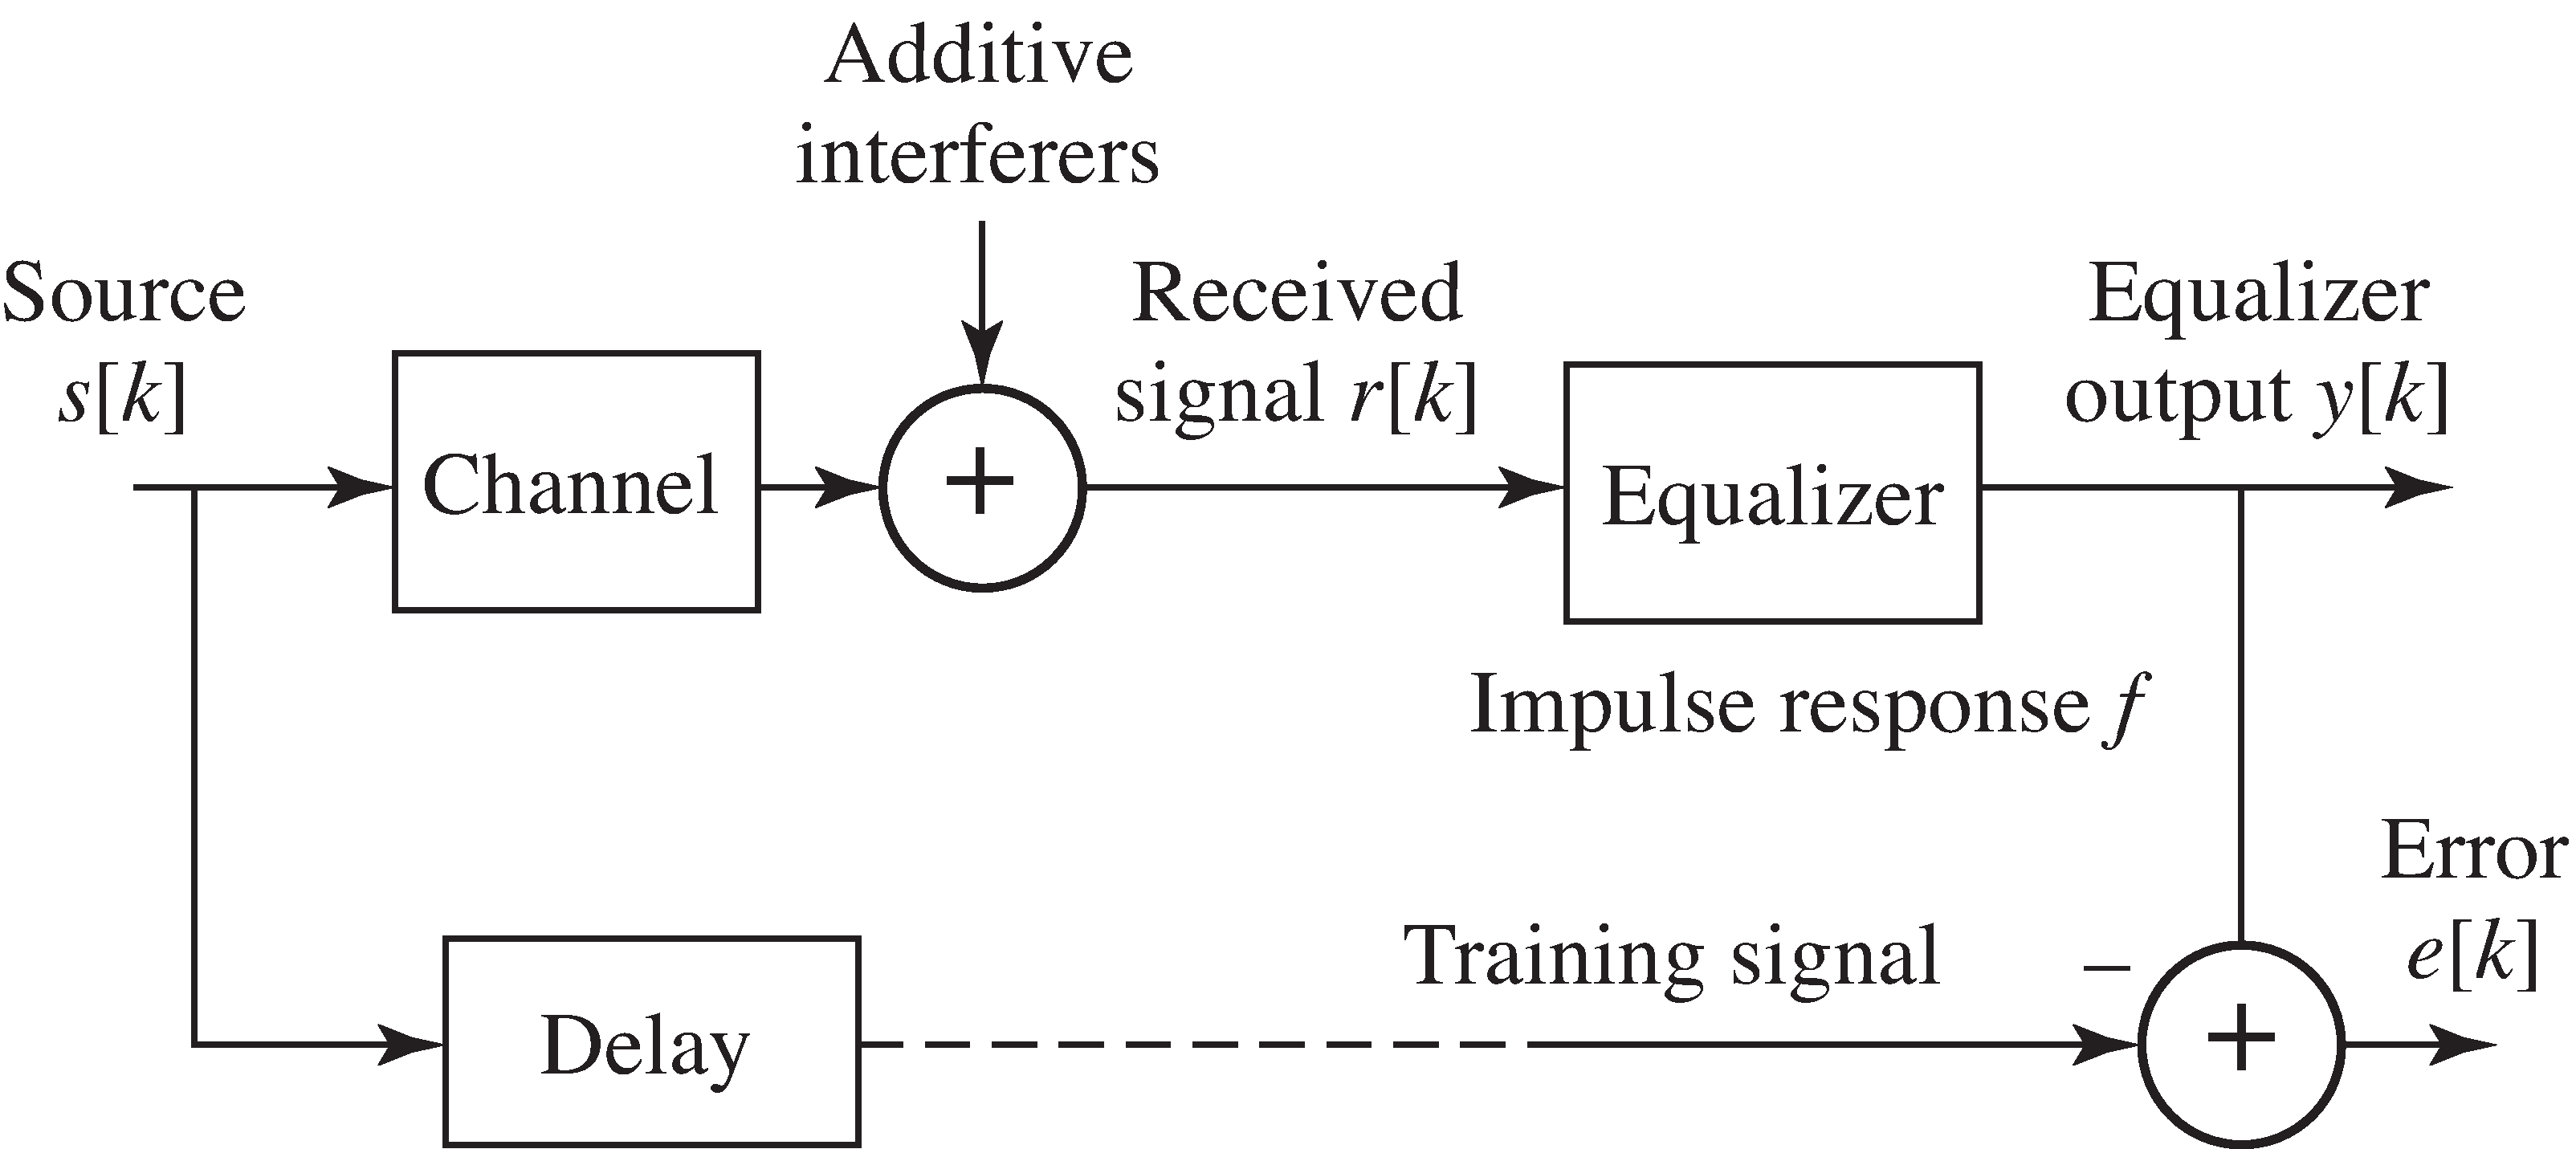
\includegraphics[width=\textwidth]{equalizer.png}
\caption{Generic Equalizer Filter to zero out the ISI\label{fig:equalizer}}
\end{figure}

%\begin{thm}
%\label{thm:zero}
%Zero-ISI:
%$$x\left(nT\right) = \left\{
%\begin{array}{1 1}
%1 & \quad n=0 \\
%0 & \quad \text{else}
%\end{array} \right.$$
%\end{thm}

%\subsection{Estimation}
%\label{sec:estimate}
%
%Considering this system, where Table~\ref{tab:filtersummary} describes the variables and Table~\ref{tab:Paramsummary} describes the dimension parameters, the channel is must be known before anything else.
%
%To do channel estimation, a known sequence is sent through the system and error on the signal at output is measured.  That is, the input ($r$) and output ($y$) of the filter are known, and the tap weights ($f$) are to be determined - we can look at the impulse response of the unknown channel facing the known input.  

\subsection{Equalization}
\label{sec:equal}
An equalizer is a filter that zeros out the ISI in the end-to-end system.  It can be preset to handle the channel, or can adapt to the time-varying nature of a channel.  In the latter case, the equalizer parameter are adjusted on the fly by periodic transmission of a known sequence to re-estimate the channel.  In either case, the equalizer is a filter whose frequency response counteracts the system model such that Condition~\ref{thm:zero} is met. 

\begin{table}[H]
\begin{center}
\begin{tabular}{|c|c|c|c|}
\hline Variable & Meaning & Dimensions \\
\hline \hline
$\vec{s}$ & Source & $m\times 1 $\\ \hline
$\vec{r}$ & Received Signal & $m\times 1$ \\ \hline
$R$ & Channel Response Matrix & $p\times n$ \\ \hline
$\vec{f}$ & Tap Line / Impulse Response & $n\times 1 $ \\ \hline
$\vec{y}$ & Equalizer Output & $ m\times 1 $ \\ \hline
 $\vec{e}$ & Training Error & $ m\times 1 $ \\ \hline
\end{tabular}
\caption{Summary of Signal Variables} \label{tab:filtersummary}
\end{center}
\end{table}

\begin{table}[B]
\begin{center}
\begin{tabular}{|c|c|}
\hline Parameter & Meaning \\
\hline \hline
$m$ & Signal Length \\ \hline
$N$ & Channel Filter Order \\ \hline
$n$ & Equalizer Filter Order \\ \hline
$p$ & Training Sequence Length \\ \hline
\end{tabular}
\caption{Summary of Parameters} \label{tab:Paramsummary}
\end{center}
\end{table}

The FIR form of the equalizer can then be written as Equation~\ref{eq:equalizerVector} and Equation~\ref{eq:equalizerMatrix}.  The compact form of this relation uses a matrix equation where the filter is expressed as a Toeplitz matrix.  This neat fact allows us to use the power of linear algebra to solve for the zero forcing channel.  
  
 
\begin{figure}[H]
\centering
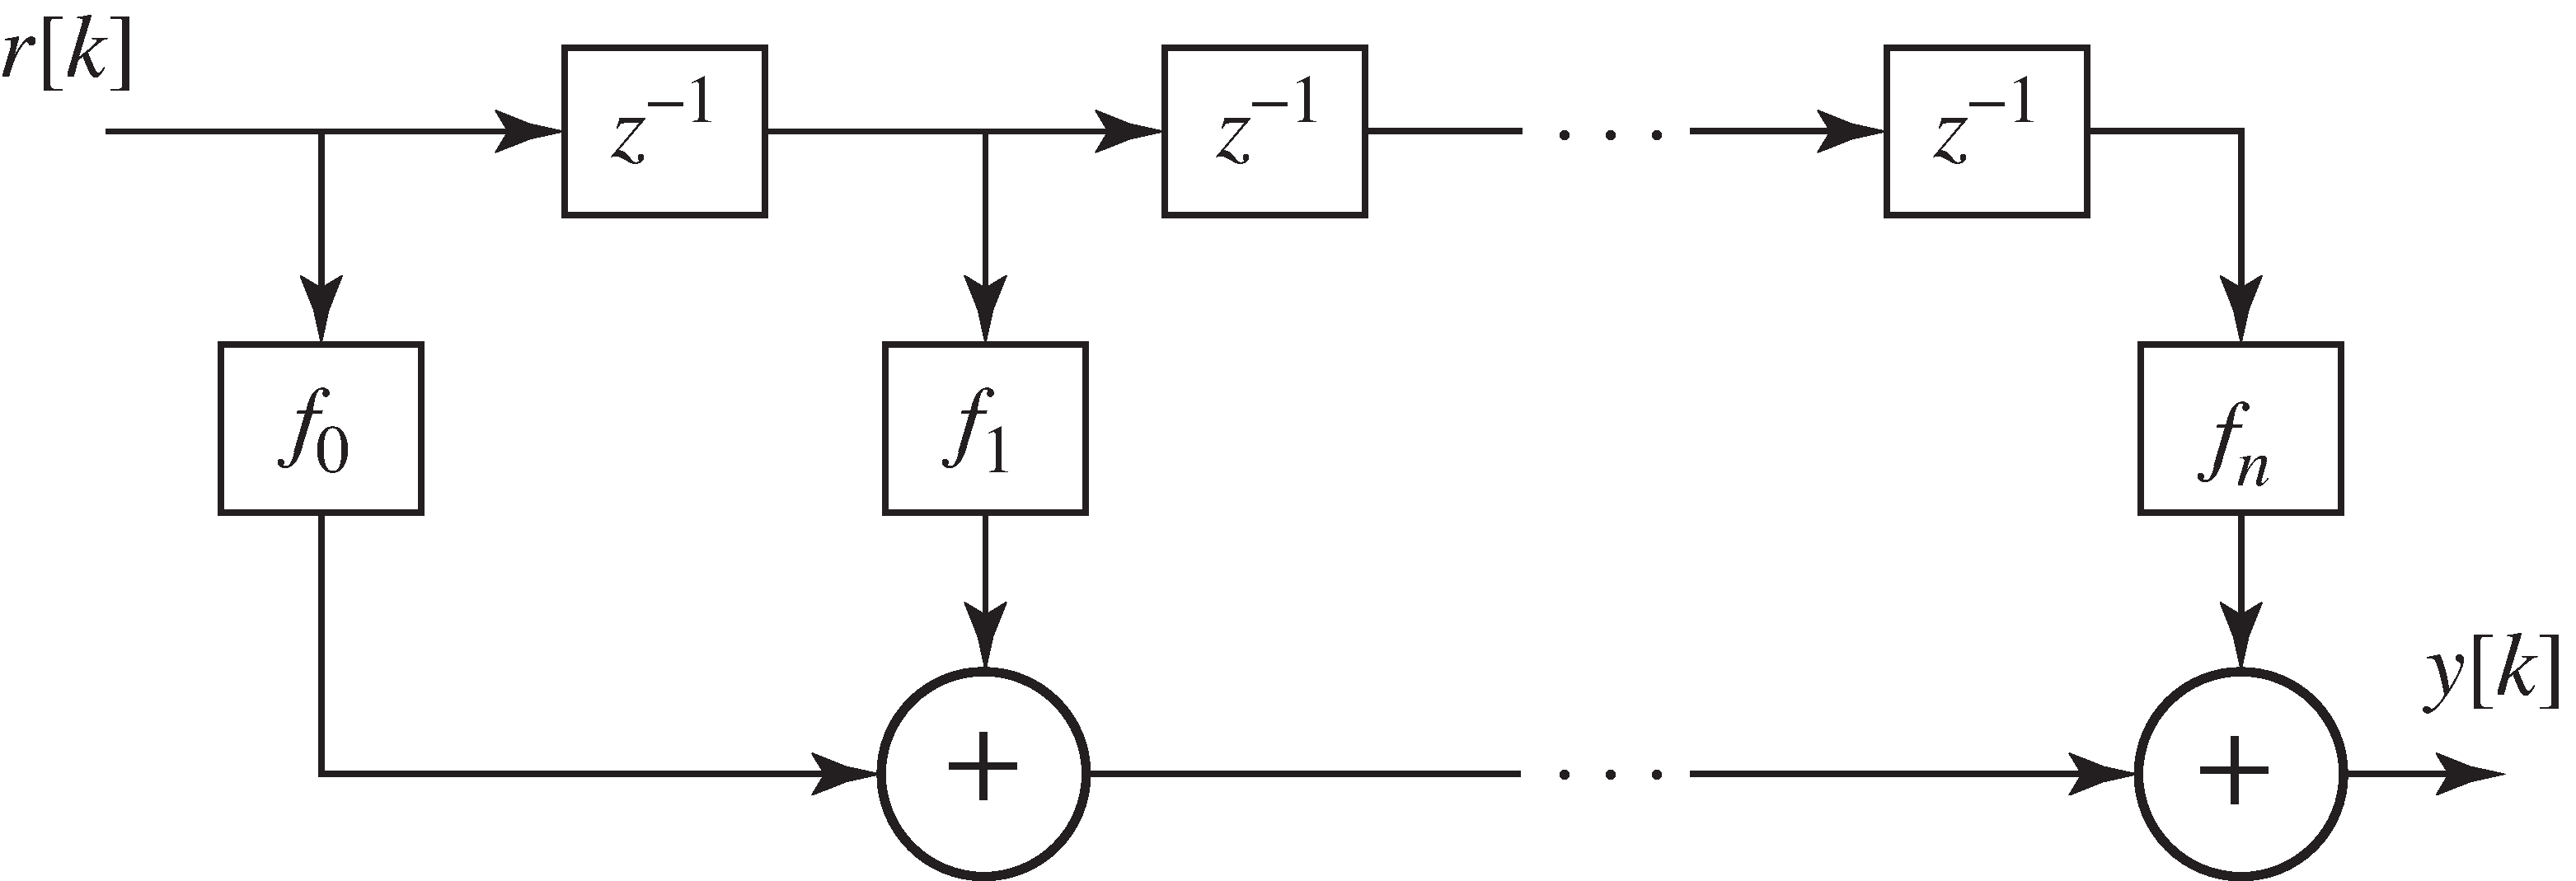
\includegraphics[width=\textwidth]{tapEqualizer.png}
\caption{Tapped Delay Line Represenation\label{fig:tap}}
\end{figure}
\begin{equation}
\label{eq:equalizer}
y\left[k\right] = \sum_{j=0}^n f_jr\left[k-j\right]
\end{equation}

The direct form of the FIR equalizor is shown in Figure~\ref{fig:tap}.  This is a subblock diagram view of the equalizer filter.  The transfer function can be seen in Equation~\ref{eq:equalizer}.  The objective for this filter is to counter the system channel.  \\

\begin{equation}
\label{eq:equalizerVector}
\left[ \begin{array}{c}
 y \left[n+1\right] \\
 y \left[n+2\right] \\
 y \left[n+3\right] \\
\vdots  \\
y\left[ p \right] \end{array} \right] = 
\begin{bmatrix} 
r \left[ n+1\right]  & r[n] \cdots & r\left[ 1 \right] \\ 
r \left[ n+2\right]  & r[n+1] \cdots & r\left[ 2 \right] \\ 
r \left[ n+2\right]  & r[n+2] \cdots & r\left[ 3 \right] \\ 
\vdots & \vdots & & \vdots \\
r \left[p \right] & r\left[ p-1 \right] & \cdots r\left[ p-n \right]
\end{bmatrix}
 \left[ \begin{array}{c} f_0 \\ f_1 \\ f_2 \\ \vdots \\ f_n \end{array} \right]
\end{equation}

\begin{equation}
\label{eq:equalizerMatrix}
\vec{y} = R\vec{f}
\end{equation}
What we want is to optimally force the channel to zero for all other symbols than the present one.  As an aside, because there is delay in the system, the intuitive sense of causality is blurred. That is, forward symbols from the present moment can actually cause interference to the present symbol.   \\

\section{Optimality}
\label{sec:optimal}
In order to find an optimal equalizer weighting function, we need to define a cost function as a metric to minimize cost, $J(\vec{f})$.  Here, we look at the Mean Square Error.  We can interpret this as the deviation of the estimate from the truth, squared [Equation~\ref{eq:mse}].  This formulation uses the $R$ matrix from before and defines the estimate error as $\vec{e} = \vec{s} - \vec{y}$.  This setting is well studied and the optimal weighting vector, $\vec{f}_{LS}$ is shown in Equation~\ref{eq:optimal}\footnote{Note that this setting assumes $R$ has more rows than columns and that such an inverse exists}.
\begin{equation}
\label{eq:mse} 
J_{MSE} \left( \vec{f}\right) = \mathbb{E} \left[ \left(\vec{s} - R \vec{f} \right)^2 \right]
\end{equation}

\begin{equation}
\label{eq:optimal}
\vec{f}^{\circ} = \left(R^{\top}R\right)^{-1}R^{\top}\vec{s}
\end{equation}

When such a weighting vector is used as the equalizer taps, the output reachse the minimum mean square error metric  [Equation~\ref{eq:mmse}].  It is interesting to note, the first term in this minimal cost function is the variance of the transmitted signal and the second term is a bias term.
\begin{equation}
\label{eq:mmse}
J_{MMSE} = \mathbb{E} \left[ \vec{s}^{\top} \vec{s} - \vec{s}^{\top} \vec{f}^{\circ} \right]
\end{equation}
\newpage
\section{System}
\label{sec:system}
The system simulation model is shown in Figure~\ref{fig:step4}.  

\begin{figure}[H]
\centering
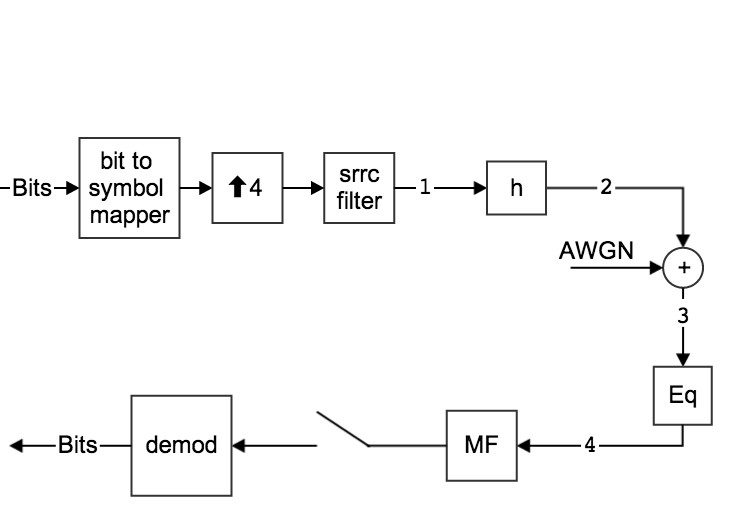
\includegraphics[width=\textwidth]{step5.png}
\caption{Block Diagram of Step 5 system setup\label{fig:step5}}
\end{figure}

As from Step 1, randomly generated bits [Appendix~\ref{app:random_bit_generator}] are converted into symbols [\ref{app:bittosym}] and then upsampled by adding in zeros [\ref{app:impulse_train}].  The result is then is run through a Square Root Raised Cosine (SRRC) pulse shape filter [\ref{app:sqrt_raised_cosine}] which is then passed through a bandlimited channel. 

\begin{equation}
\label{eq:channel}
r\left[k\right] = \sum_{j=0}^N h[j]s\left[k-j\right]
\end{equation}


We have used the following bandlimited channel responses in this step of the project:

\begin{itemize}
\item $h_1(t) = 1\delta(t) - 0.25\delta(t - T_{sym})  $
\item $h_2(t) = 1\delta(t) - 0.25\delta(t - T_{sym})   + 0.125\delta(t - 2T_{sym}) $
\item $h_3(t) = 0.1\delta(t + T_{sym}) +1\delta(t - T_{sym}) - 0.25\delta(t - T_{sym})   $
\end{itemize} 

Now that we have a channel response that is non-ideal we need to do equalization which as mentioned previously is essentially convolving the sampled signal with the inverse of the channel reponse as shown below: 

\begin{equation}
\label{eq:channel}
y\left[k\right] = \sum_{j=0}^N c[j]r\left[k-j\right]
\end{equation}

%First, to predetermine the channel, we send a delayed version of the transmitted signal, or a \emph{training} sequence, to create a metric of the channel.  We convolve the input with the unknown channel impulse response, or tap filter coefficients, to come up with the output.  This is shown in \ref{eq:channel}.  Here we  

%Since the input is known and the output is measured, we can back-out the values of the filter coefficients.  \\

%With the system channel modeled, we introduce AWGN noise into the game.  We can do this because, even if the noise was colored, we could apply a noise-whitening filter.  Assume here, however, that the noise is already white.   



In order to equalize the effects of the channels given above three different equalizers are tried out: 

\begin{itemize}
\item ZF equalizer \\

$c_{ZF} = U(U^HU)^{-1}e$ \\

\item MMSE equalizer \\

$c_{MMSE} = (U^HU + N_oI)^{-1}U^He$ \\

\item MMSE-DFE equalizer

$c_{LS} = \hat{R}^{-1}\hat{p} $ \\

$ \hat{R} = \frac{1}{N} \sum_{n=1}^N r[n](r[n])^H, \; \hat{p} = \frac{1}{N}\sum_{n=1}^N b^*[n]r[n]$ \\


\end{itemize}


The end of the simulation model is identical to the process in Step 1: a matched filter to the SRRC picks out the symbols from the noisy received signal.  Afterwards, a sampler recovers [Appendix~\ref{app:sampler}] the symbols before a demodulator converts the symbols back into bits [\ref{app:dblocks}].  






\section{Step 5 Results}
\label{sec:results}
In the following sections, the results of the simulations of the different modulation schemes are shown. 

\subsection{Probability Error Rate Comparison}
\label{sec:compare}

\subsubsection{BPSK}

\begin{figure}[H]
\centering
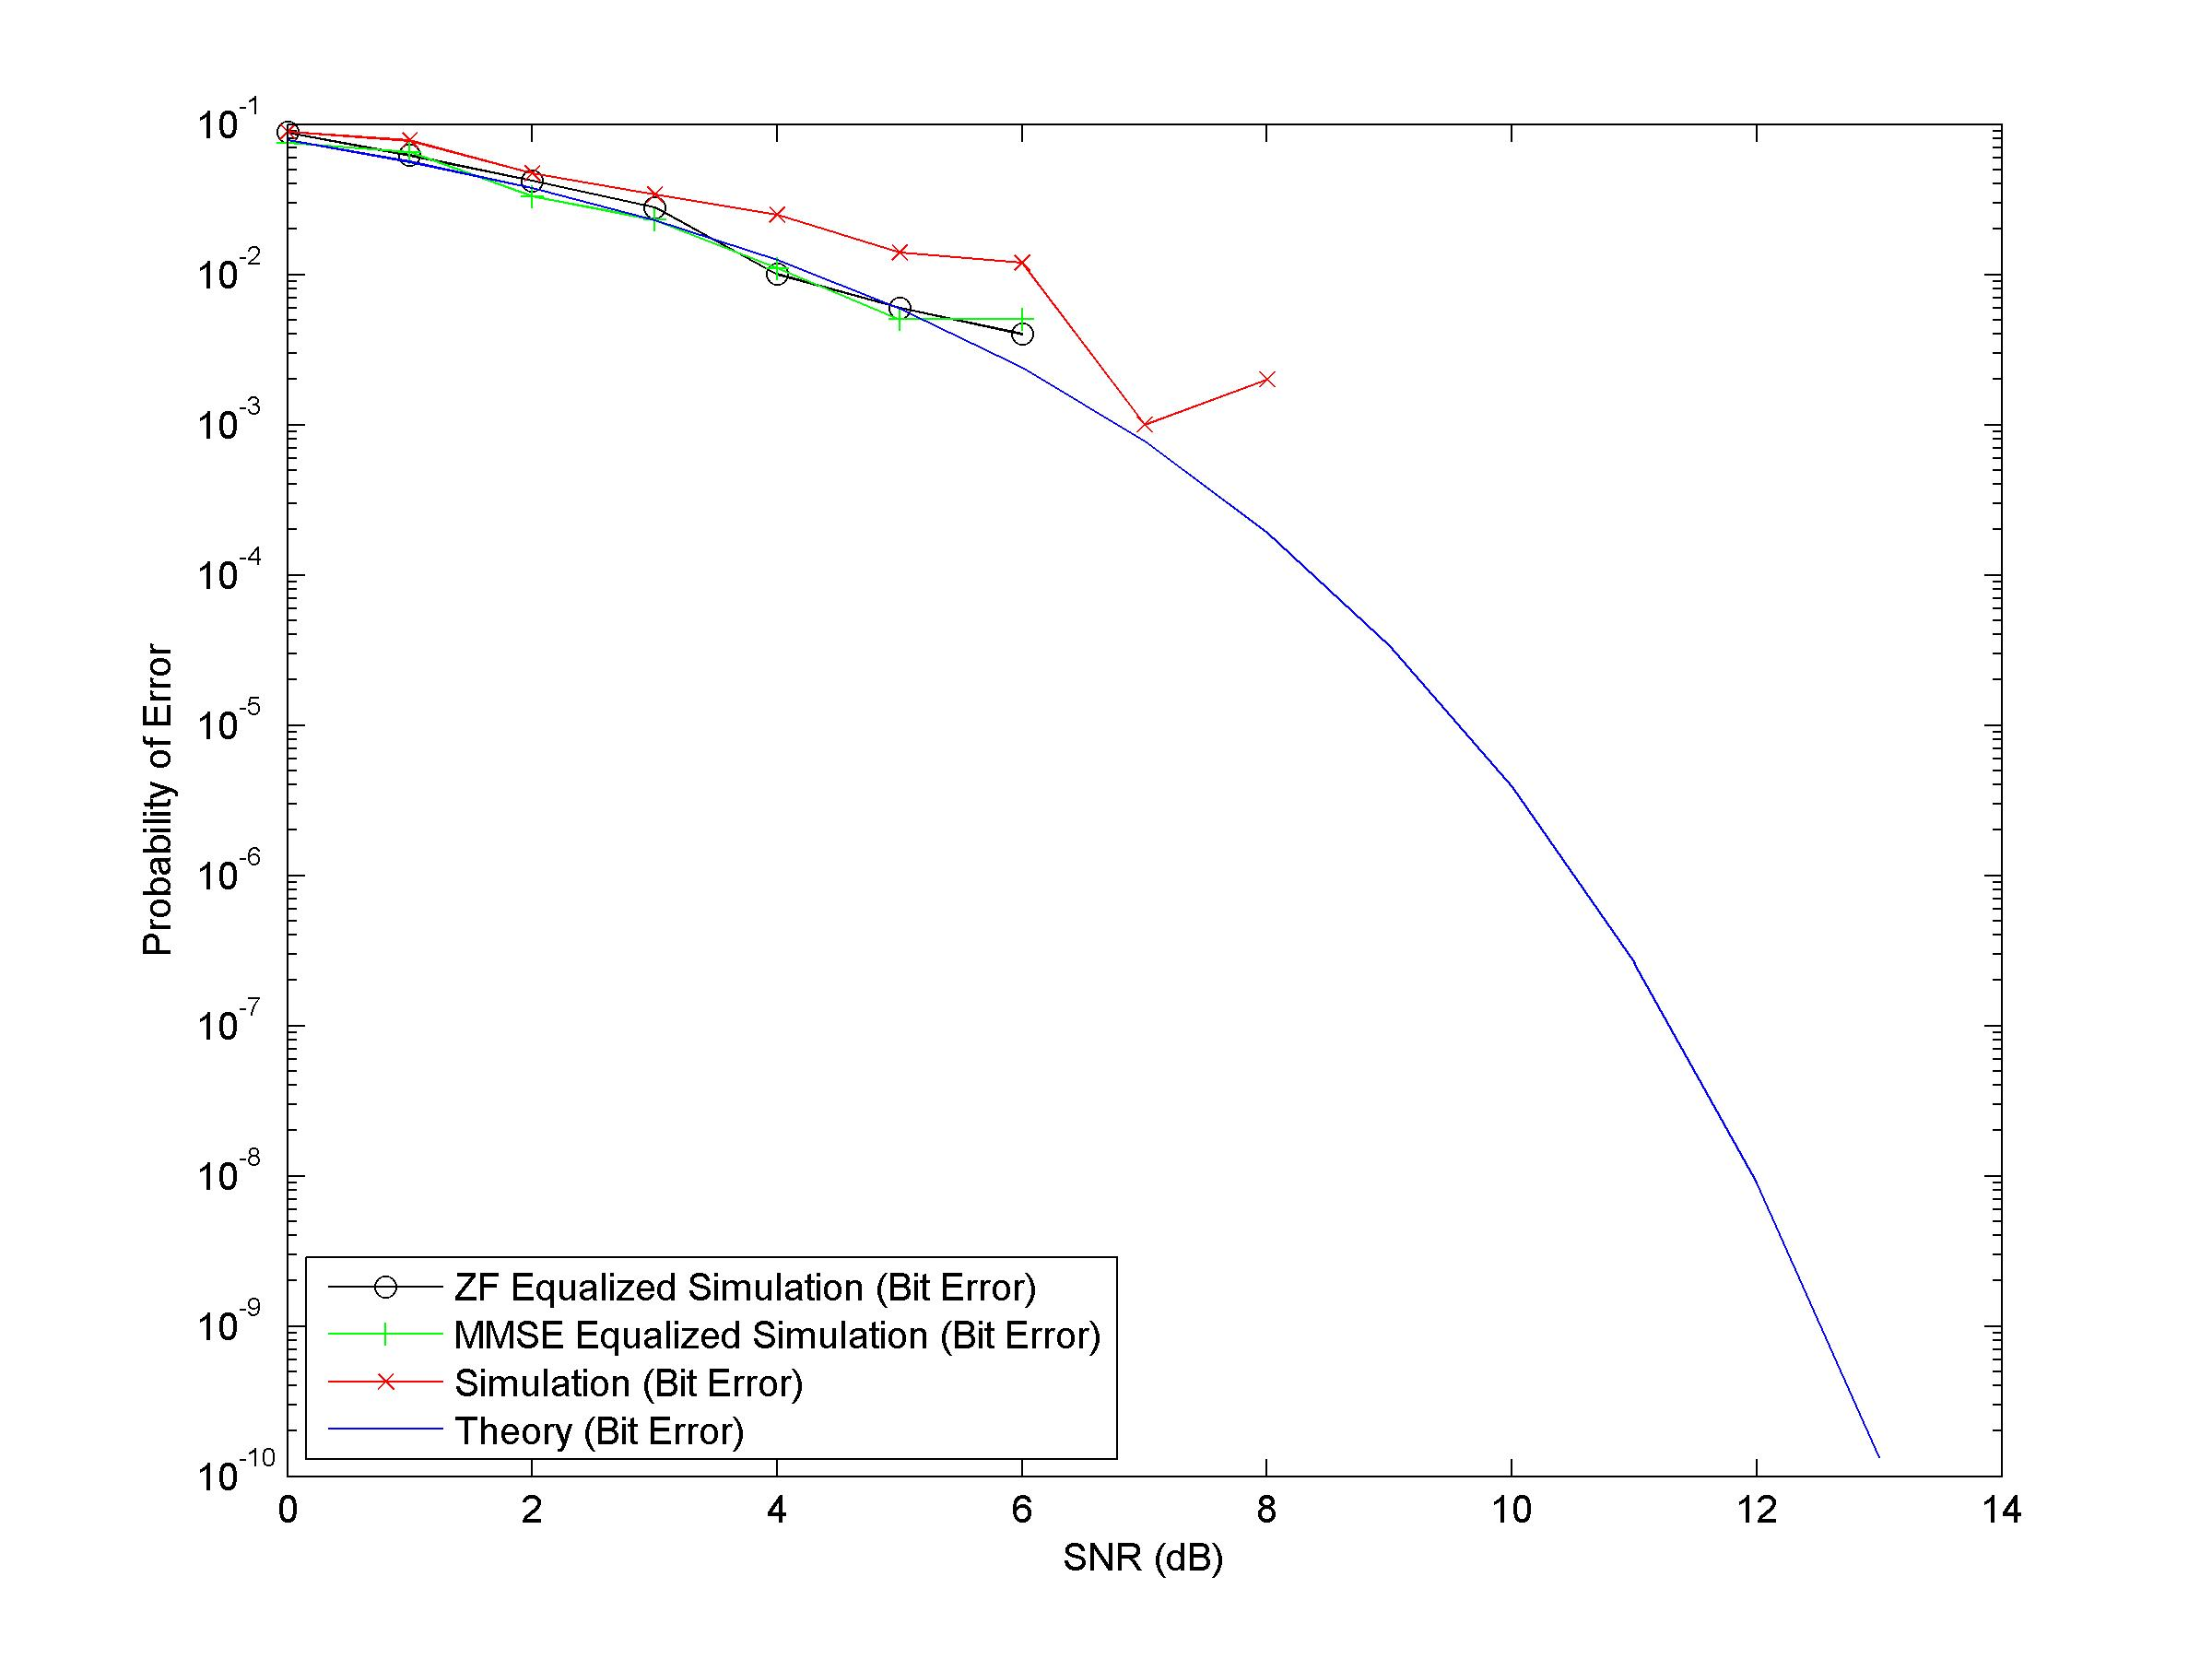
\includegraphics[width=0.7\textwidth]{bpSNR1.jpg}
\caption{Comparison of BER for BPSK system with different equalizers under channel response $h_1(t)$}
\end{figure}

\begin{figure}[H]
\centering
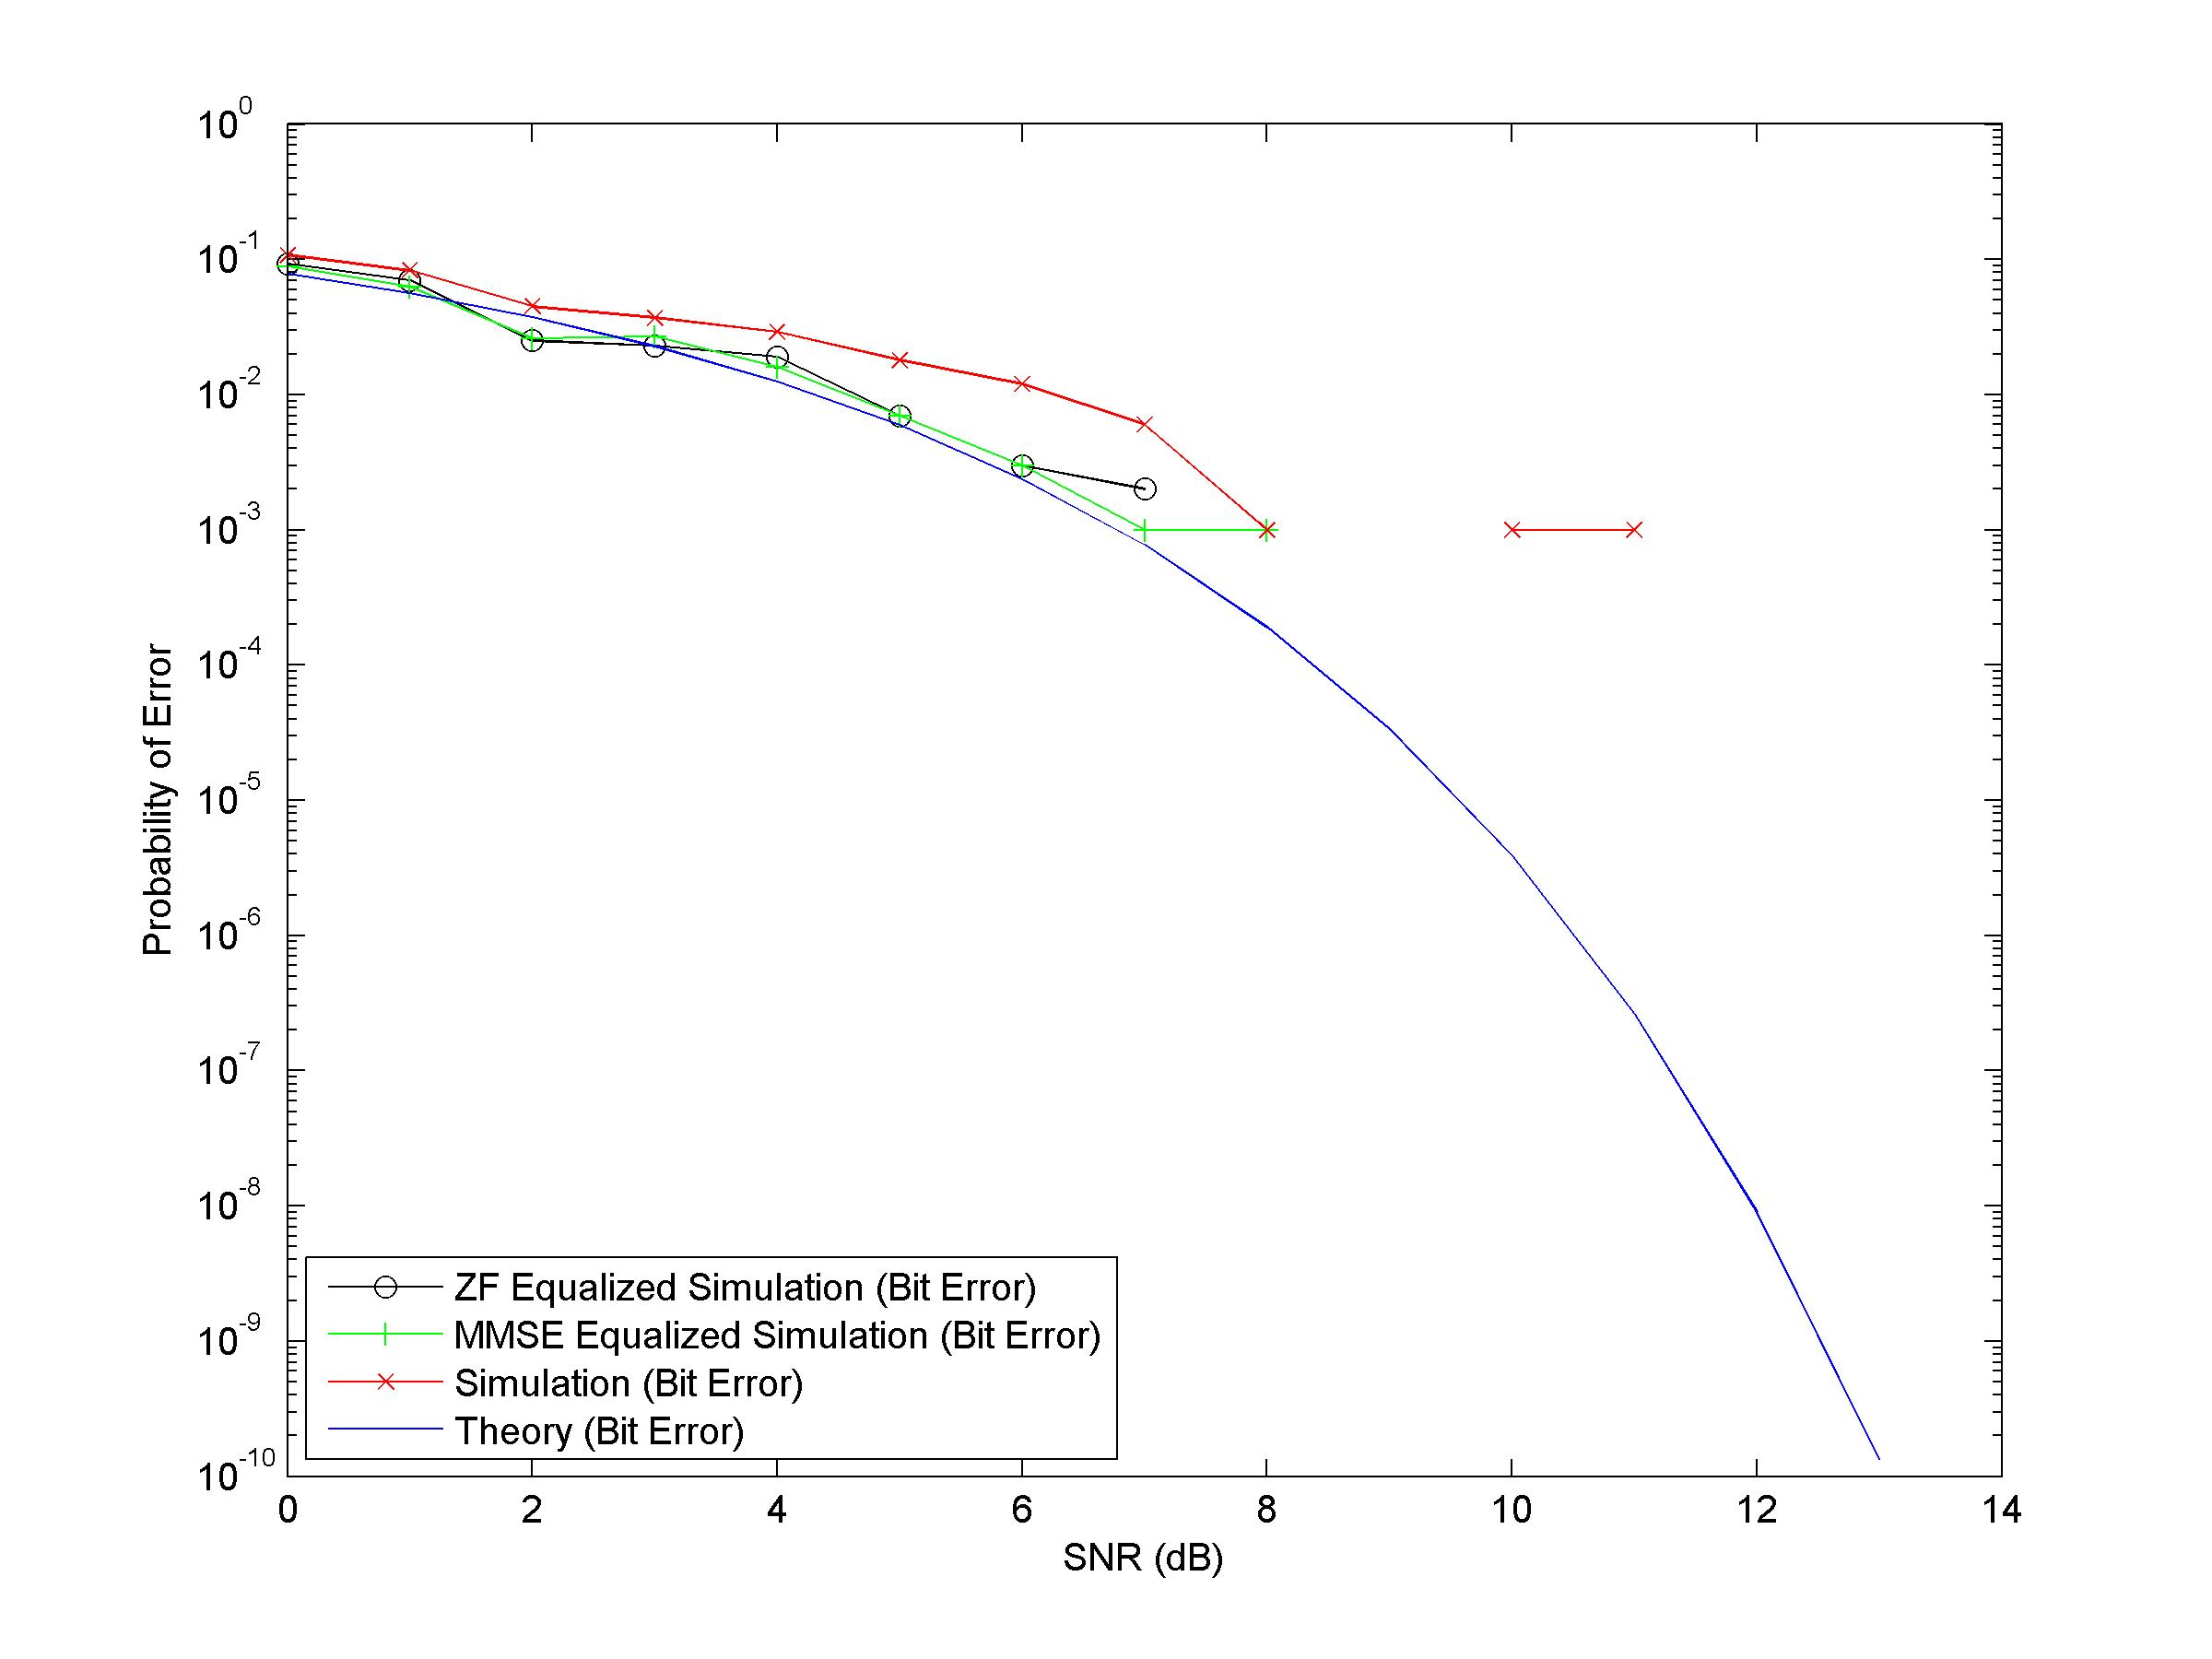
\includegraphics[width=0.7\textwidth]{bpSNR2.jpg}
\caption{Comparison of BER for BPSK system with different equalizers under channel response $h_2(t)$}
\end{figure}

\begin{figure}[H]
\centering
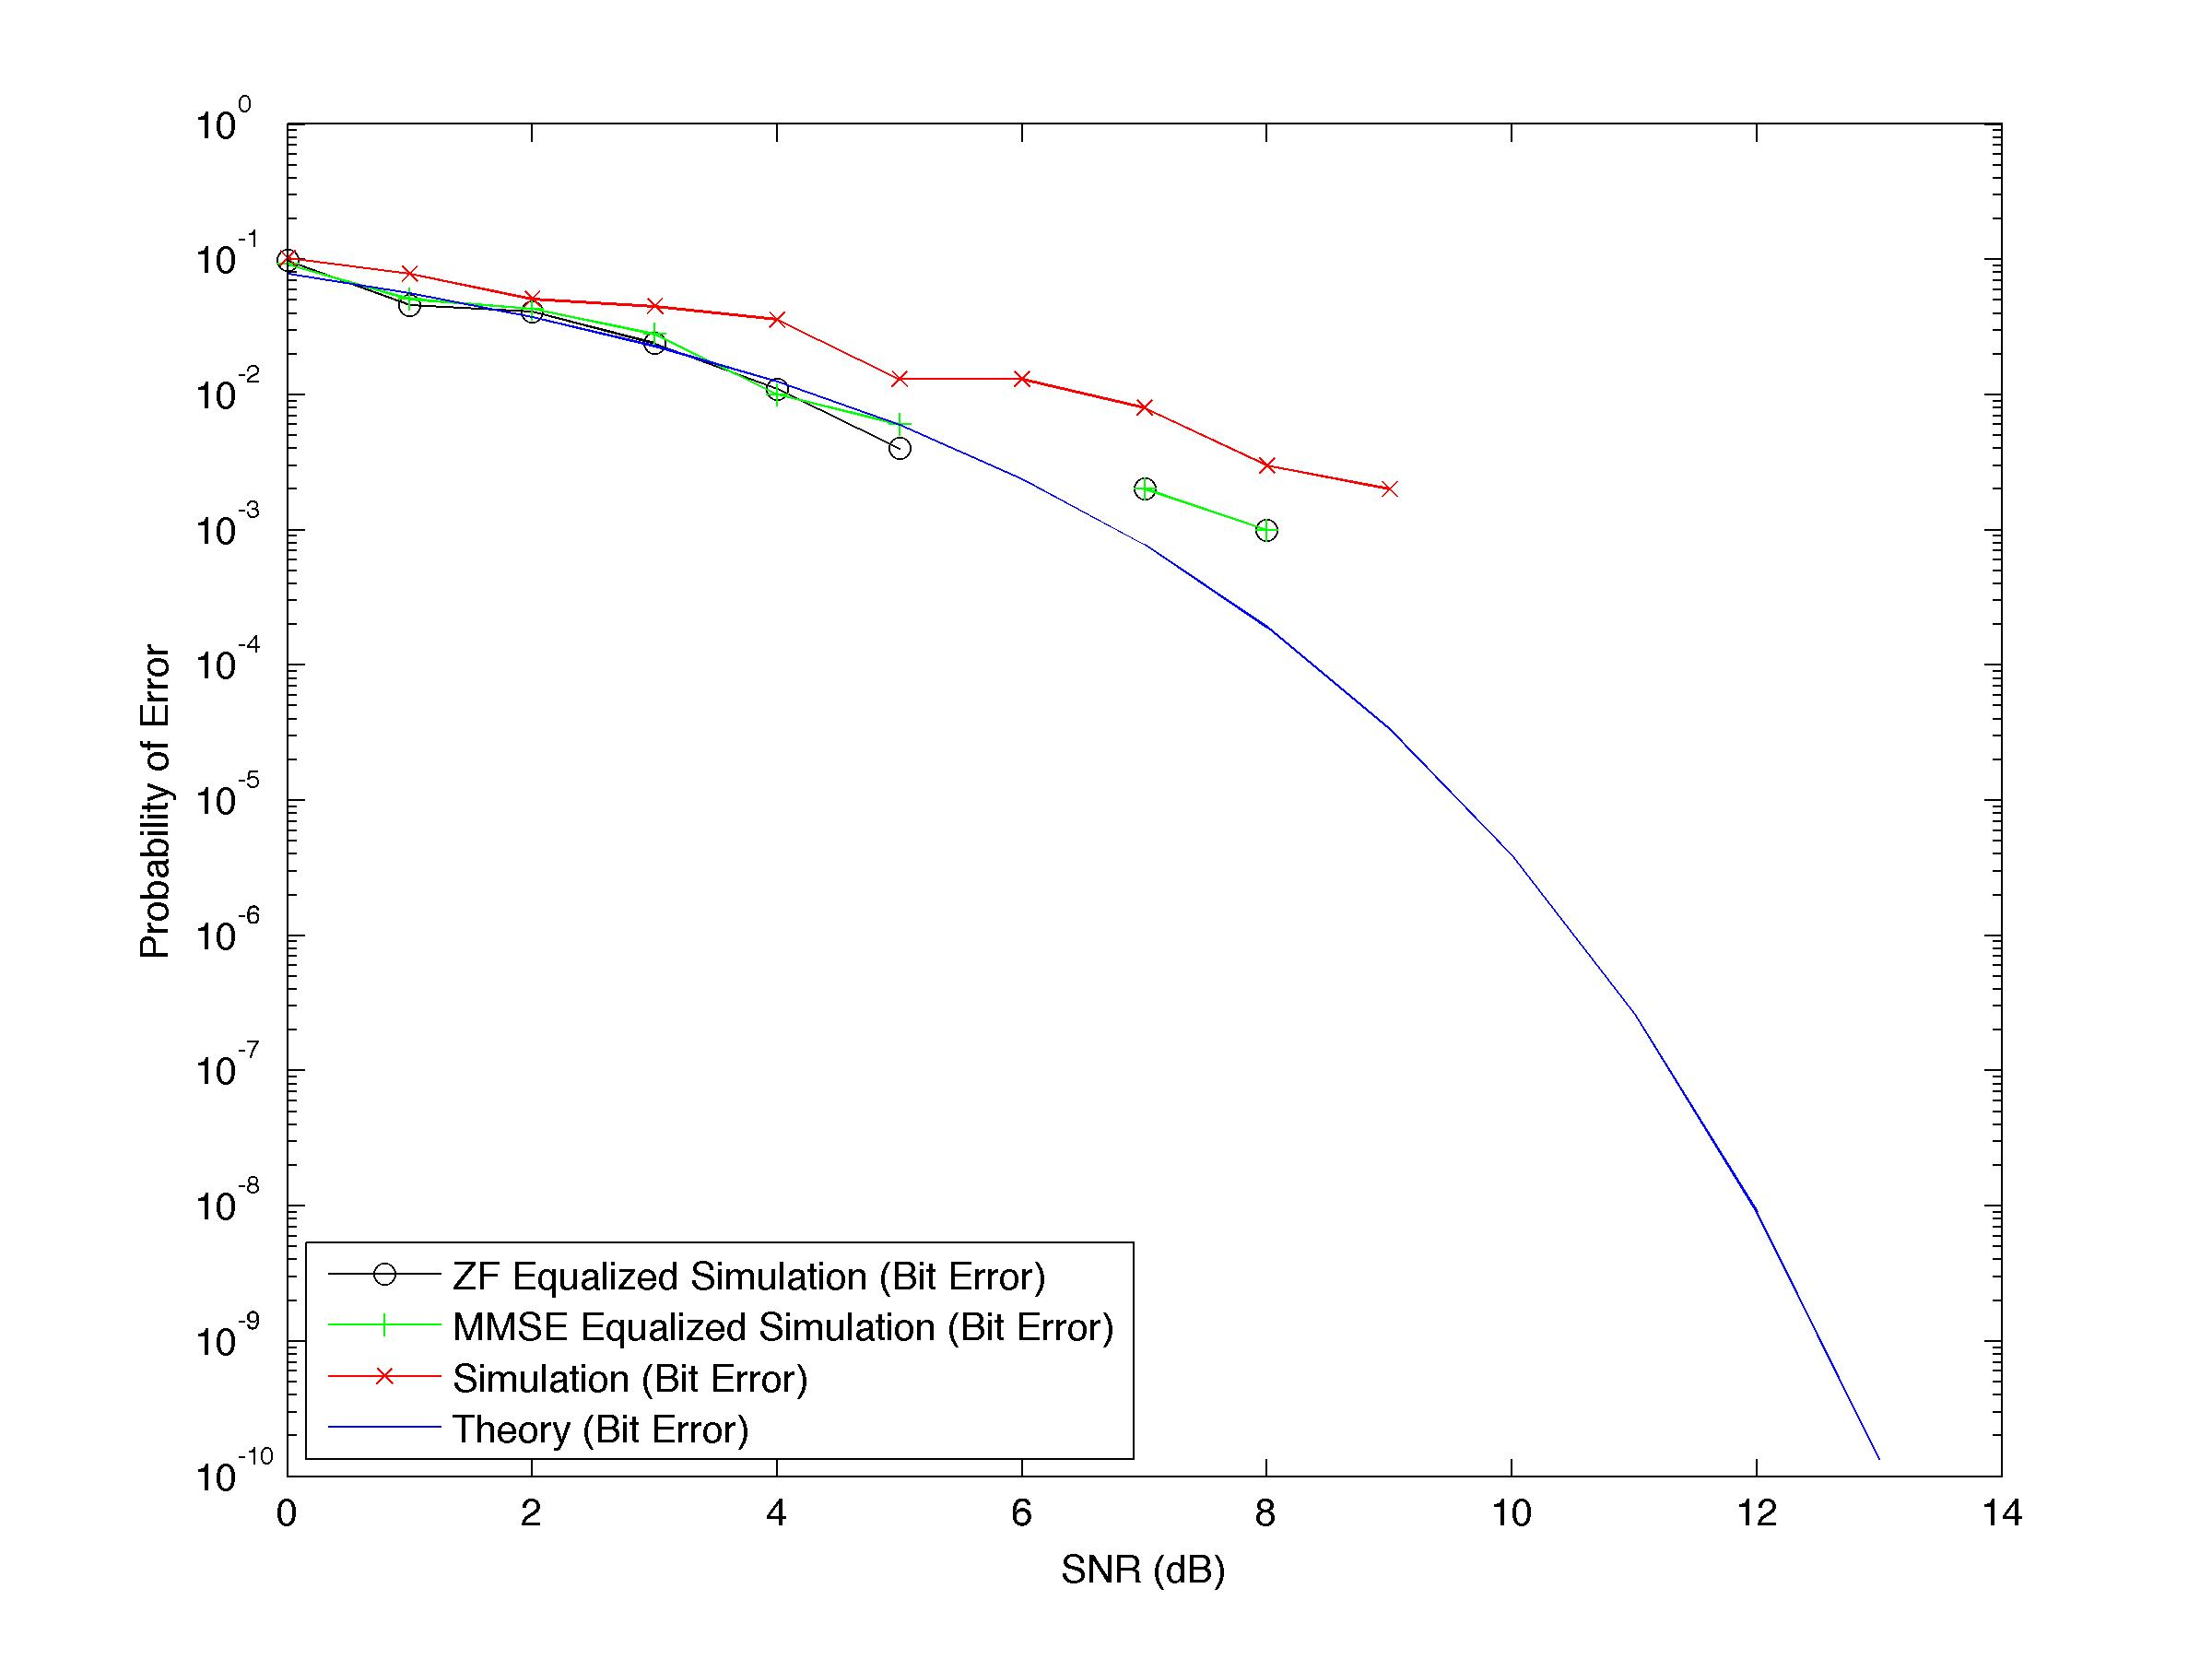
\includegraphics[width=0.7\textwidth]{bpSNR3.jpg}
\caption{Comparison of BER for BPSK system with different equalizers under channel response $h_3(t)$}
\end{figure}

\subsubsection{QPSK}

\begin{figure}[H]
\centering
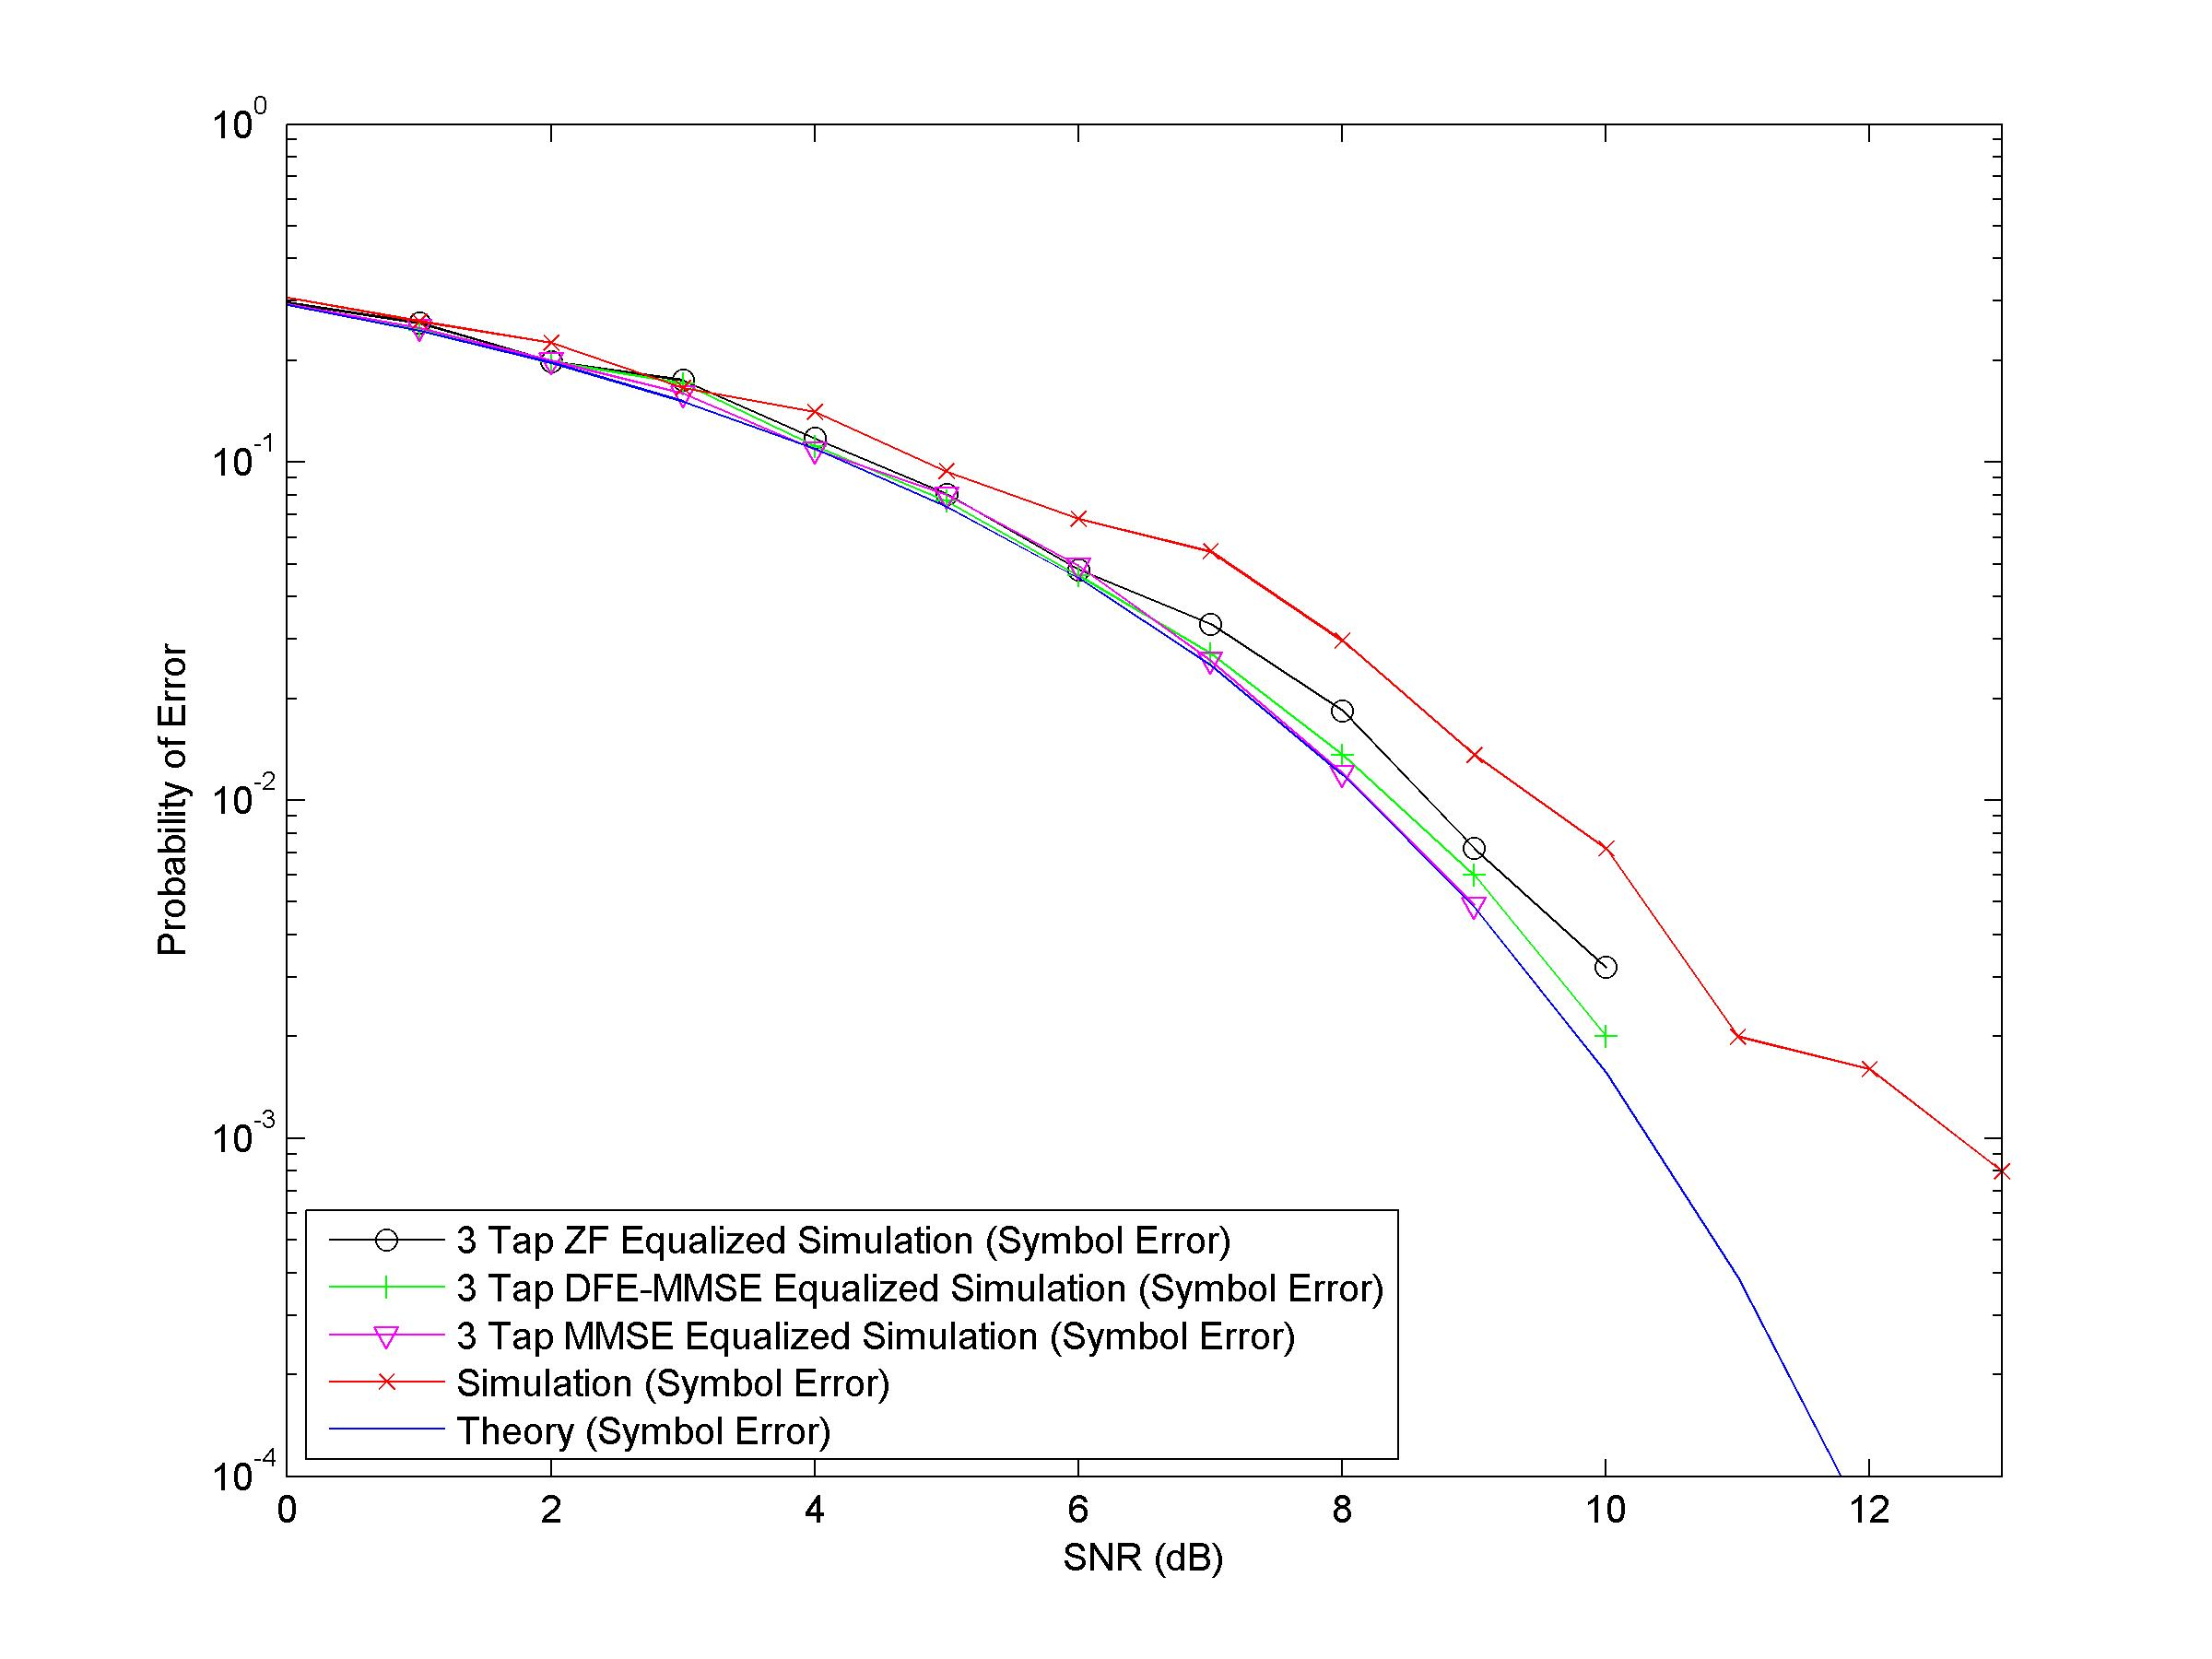
\includegraphics[width=0.7\textwidth]{qpSNR1.jpg}
\caption{Comparison of SER for QPSK system with different equalizers under channel response $h_1(t)$}
\end{figure}

\begin{figure}[H]
\centering
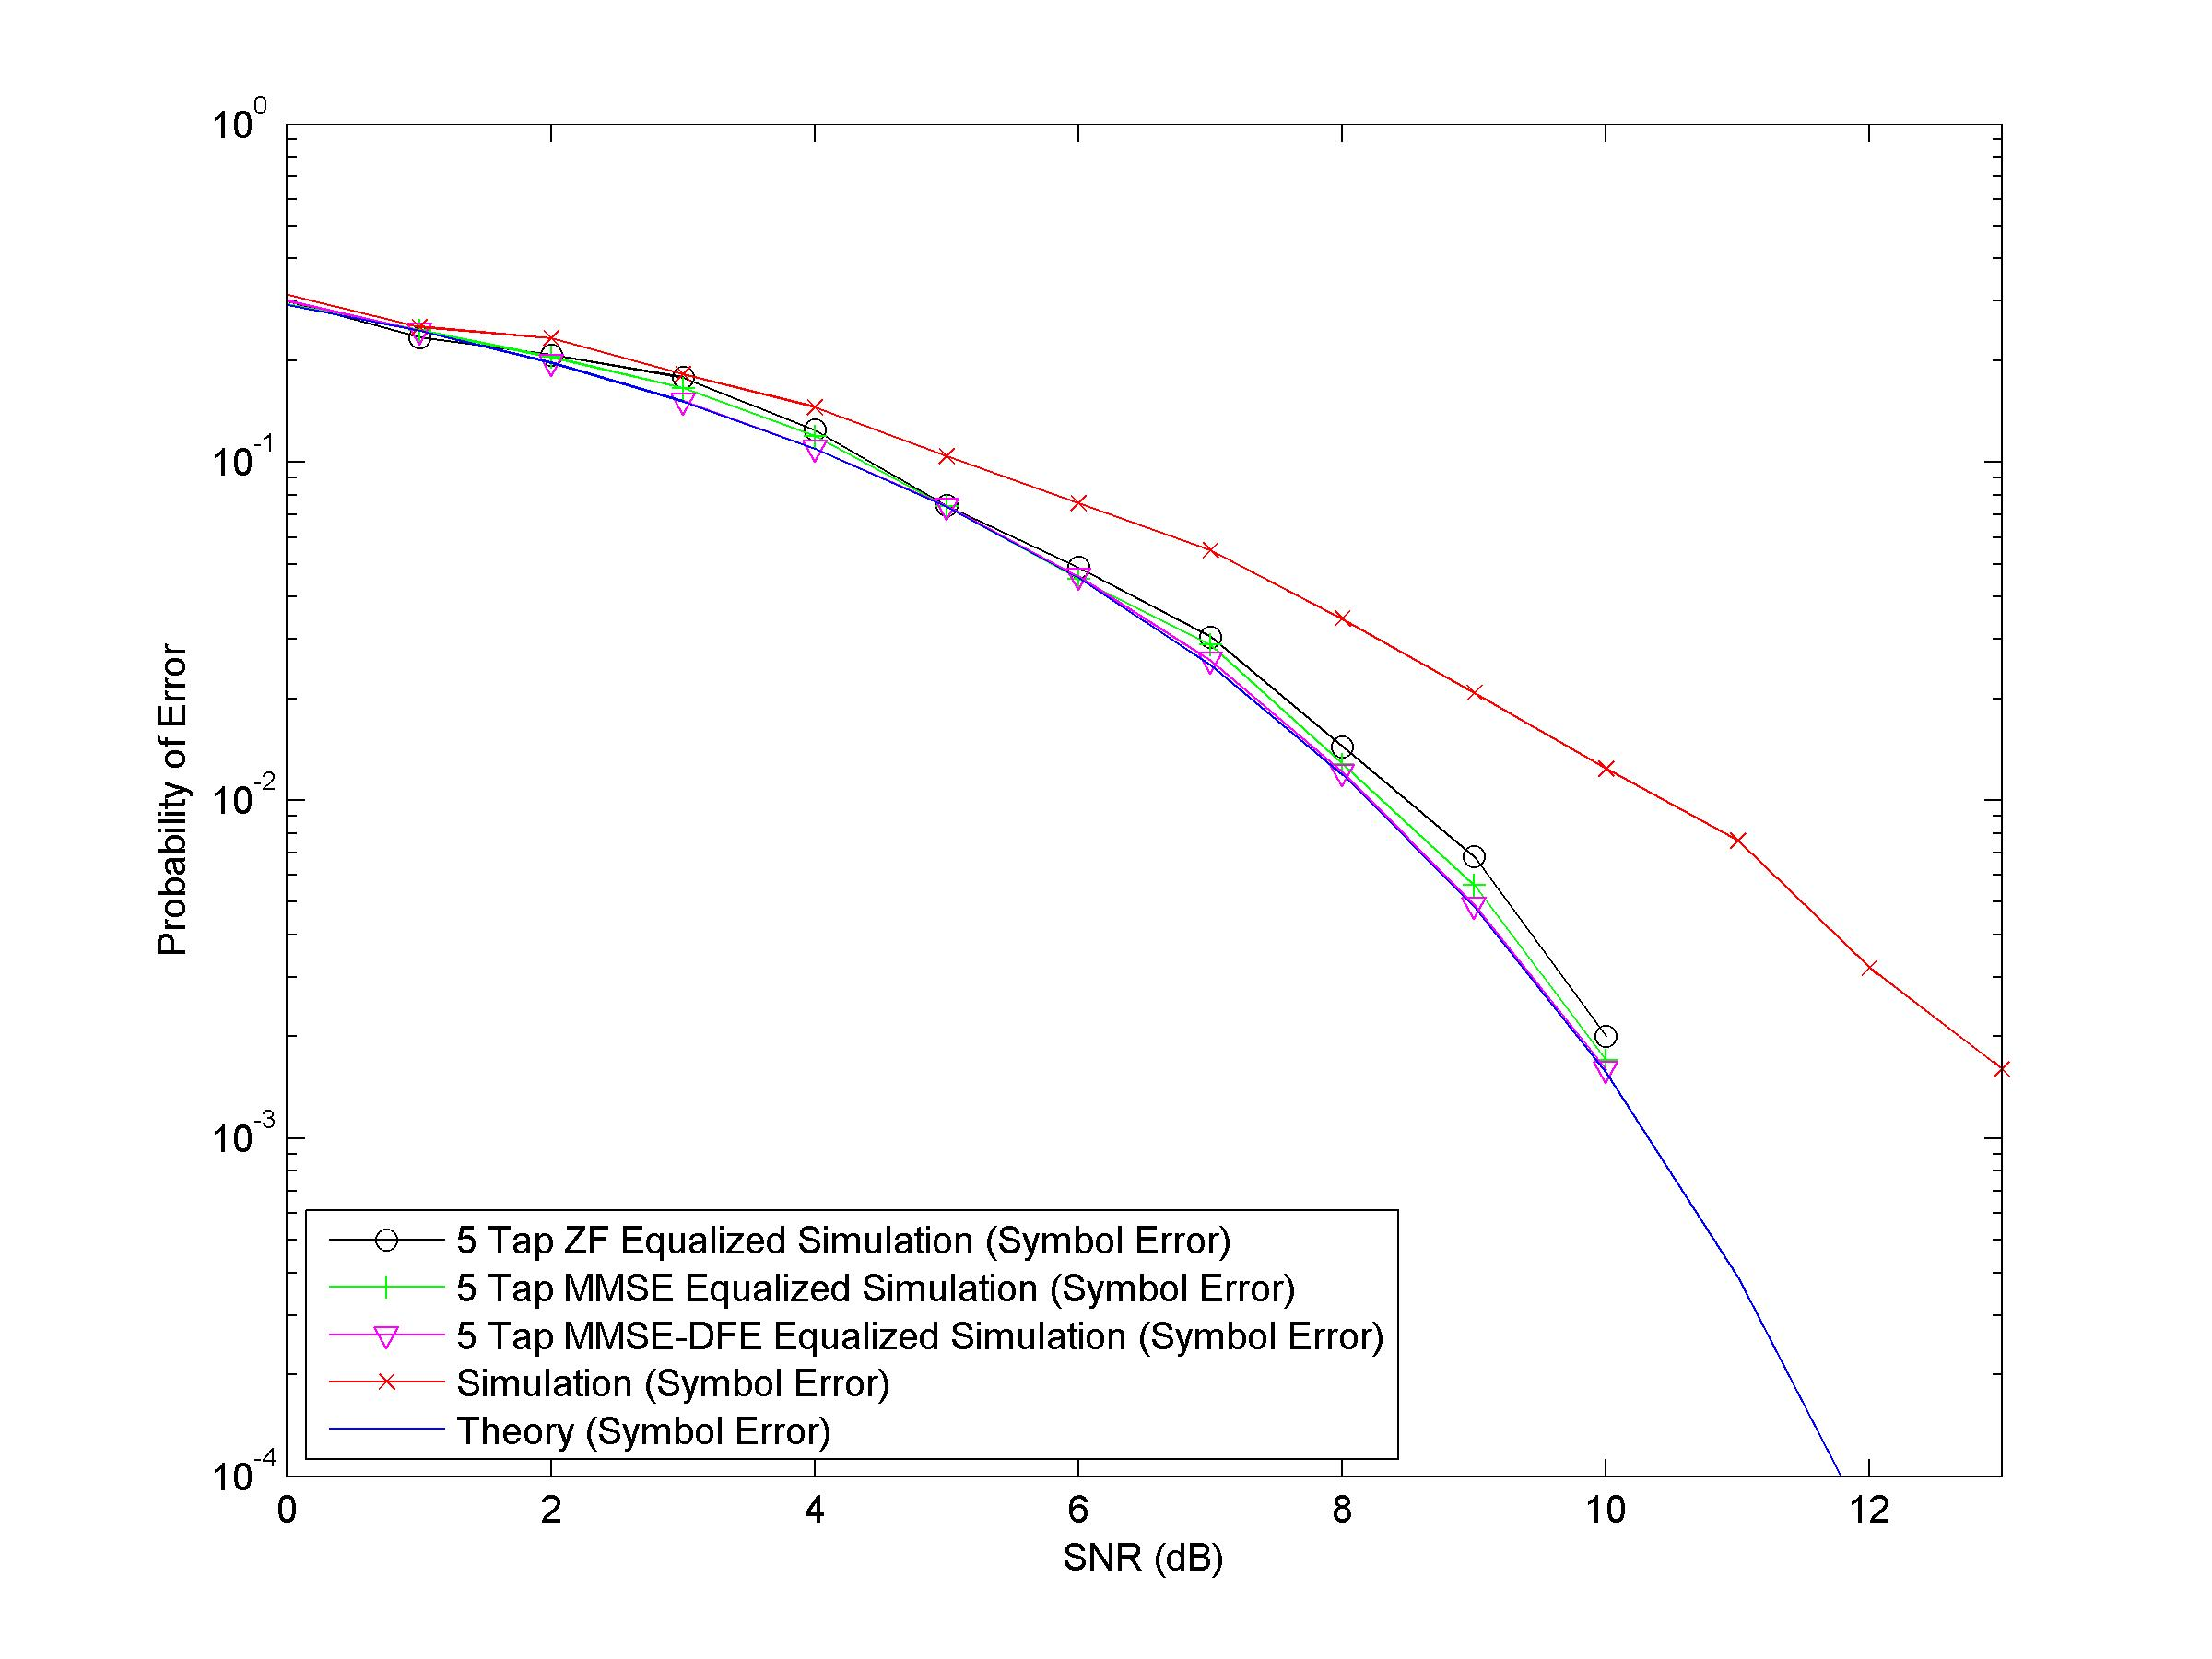
\includegraphics[width=0.7\textwidth]{qpSNR2.jpg}
\caption{Comparison of SER for QPSK system with different equalizers under channel response $h_2(t)$}
\end{figure}

\begin{figure}[H]
\centering
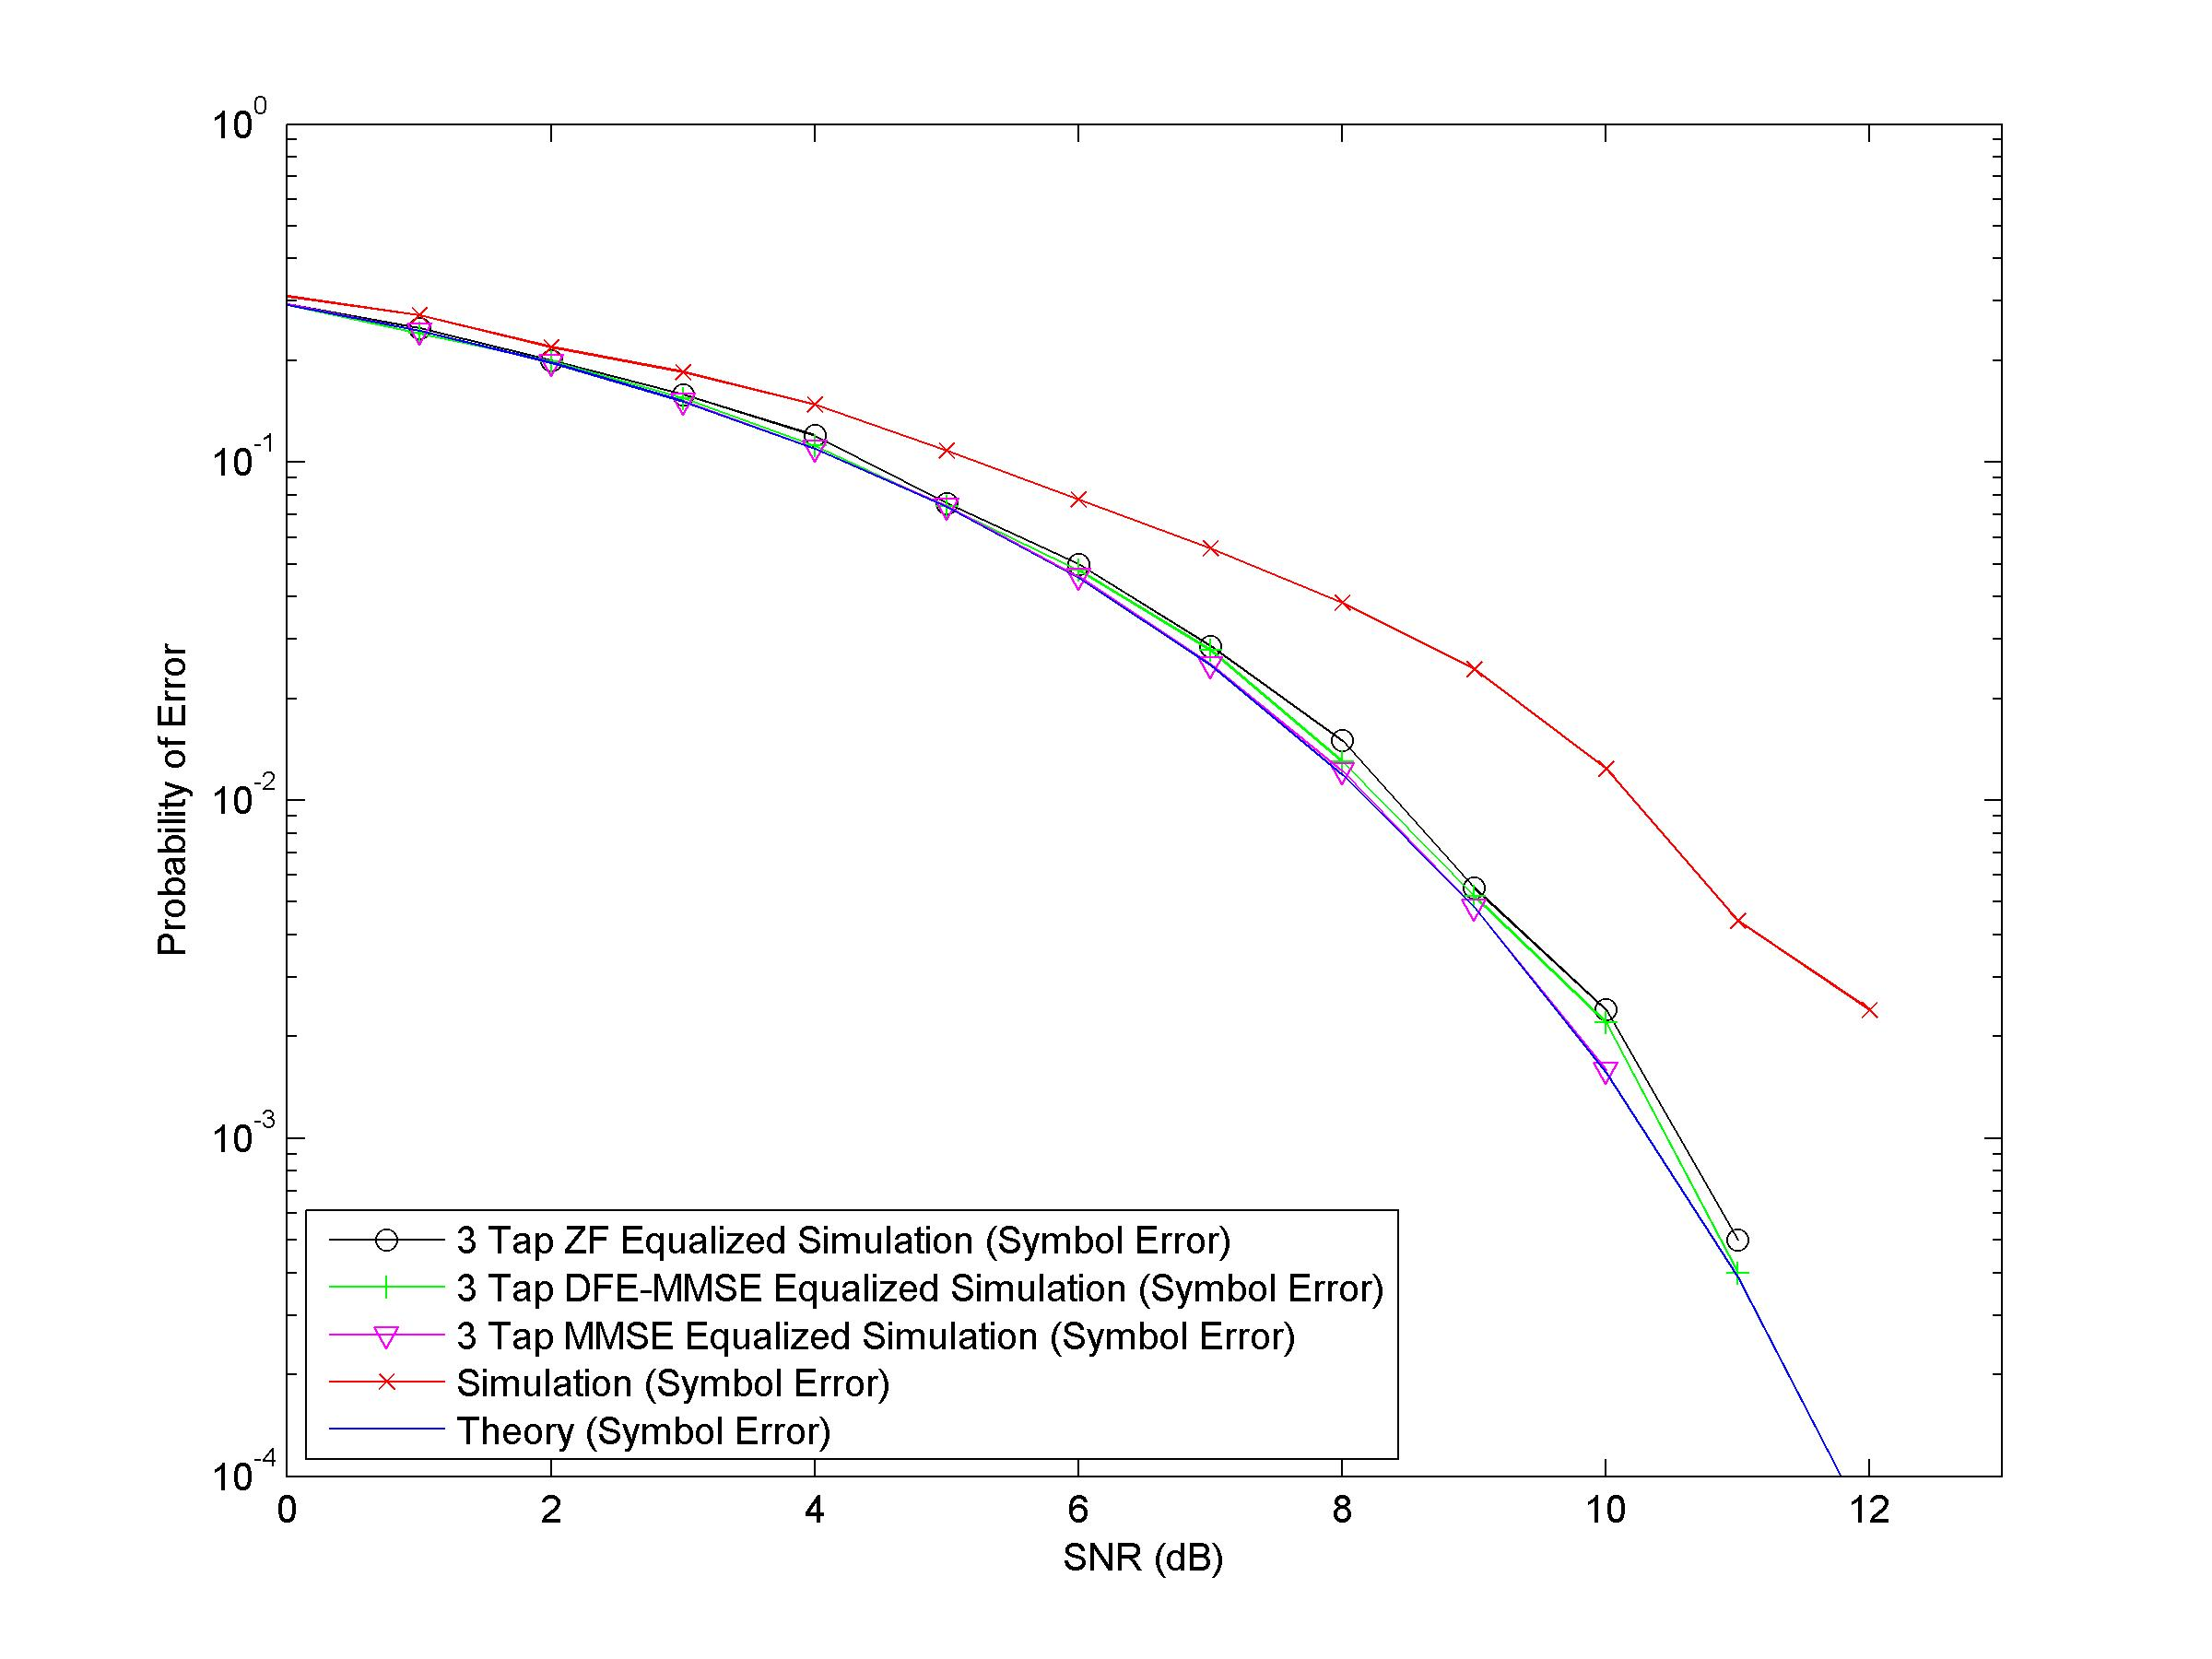
\includegraphics[width=0.7\textwidth]{qpSNR3.jpg}
\caption{Comparison of SER for QPSK system with different equalizers under channel response $h_3(t)$}
\end{figure}

\newpage
\subsection{Constellation Comparison}
\label{sec:constCompare}

\subsubsection{BPSK with No Equalization}

\begin{figure}[H]
\centering
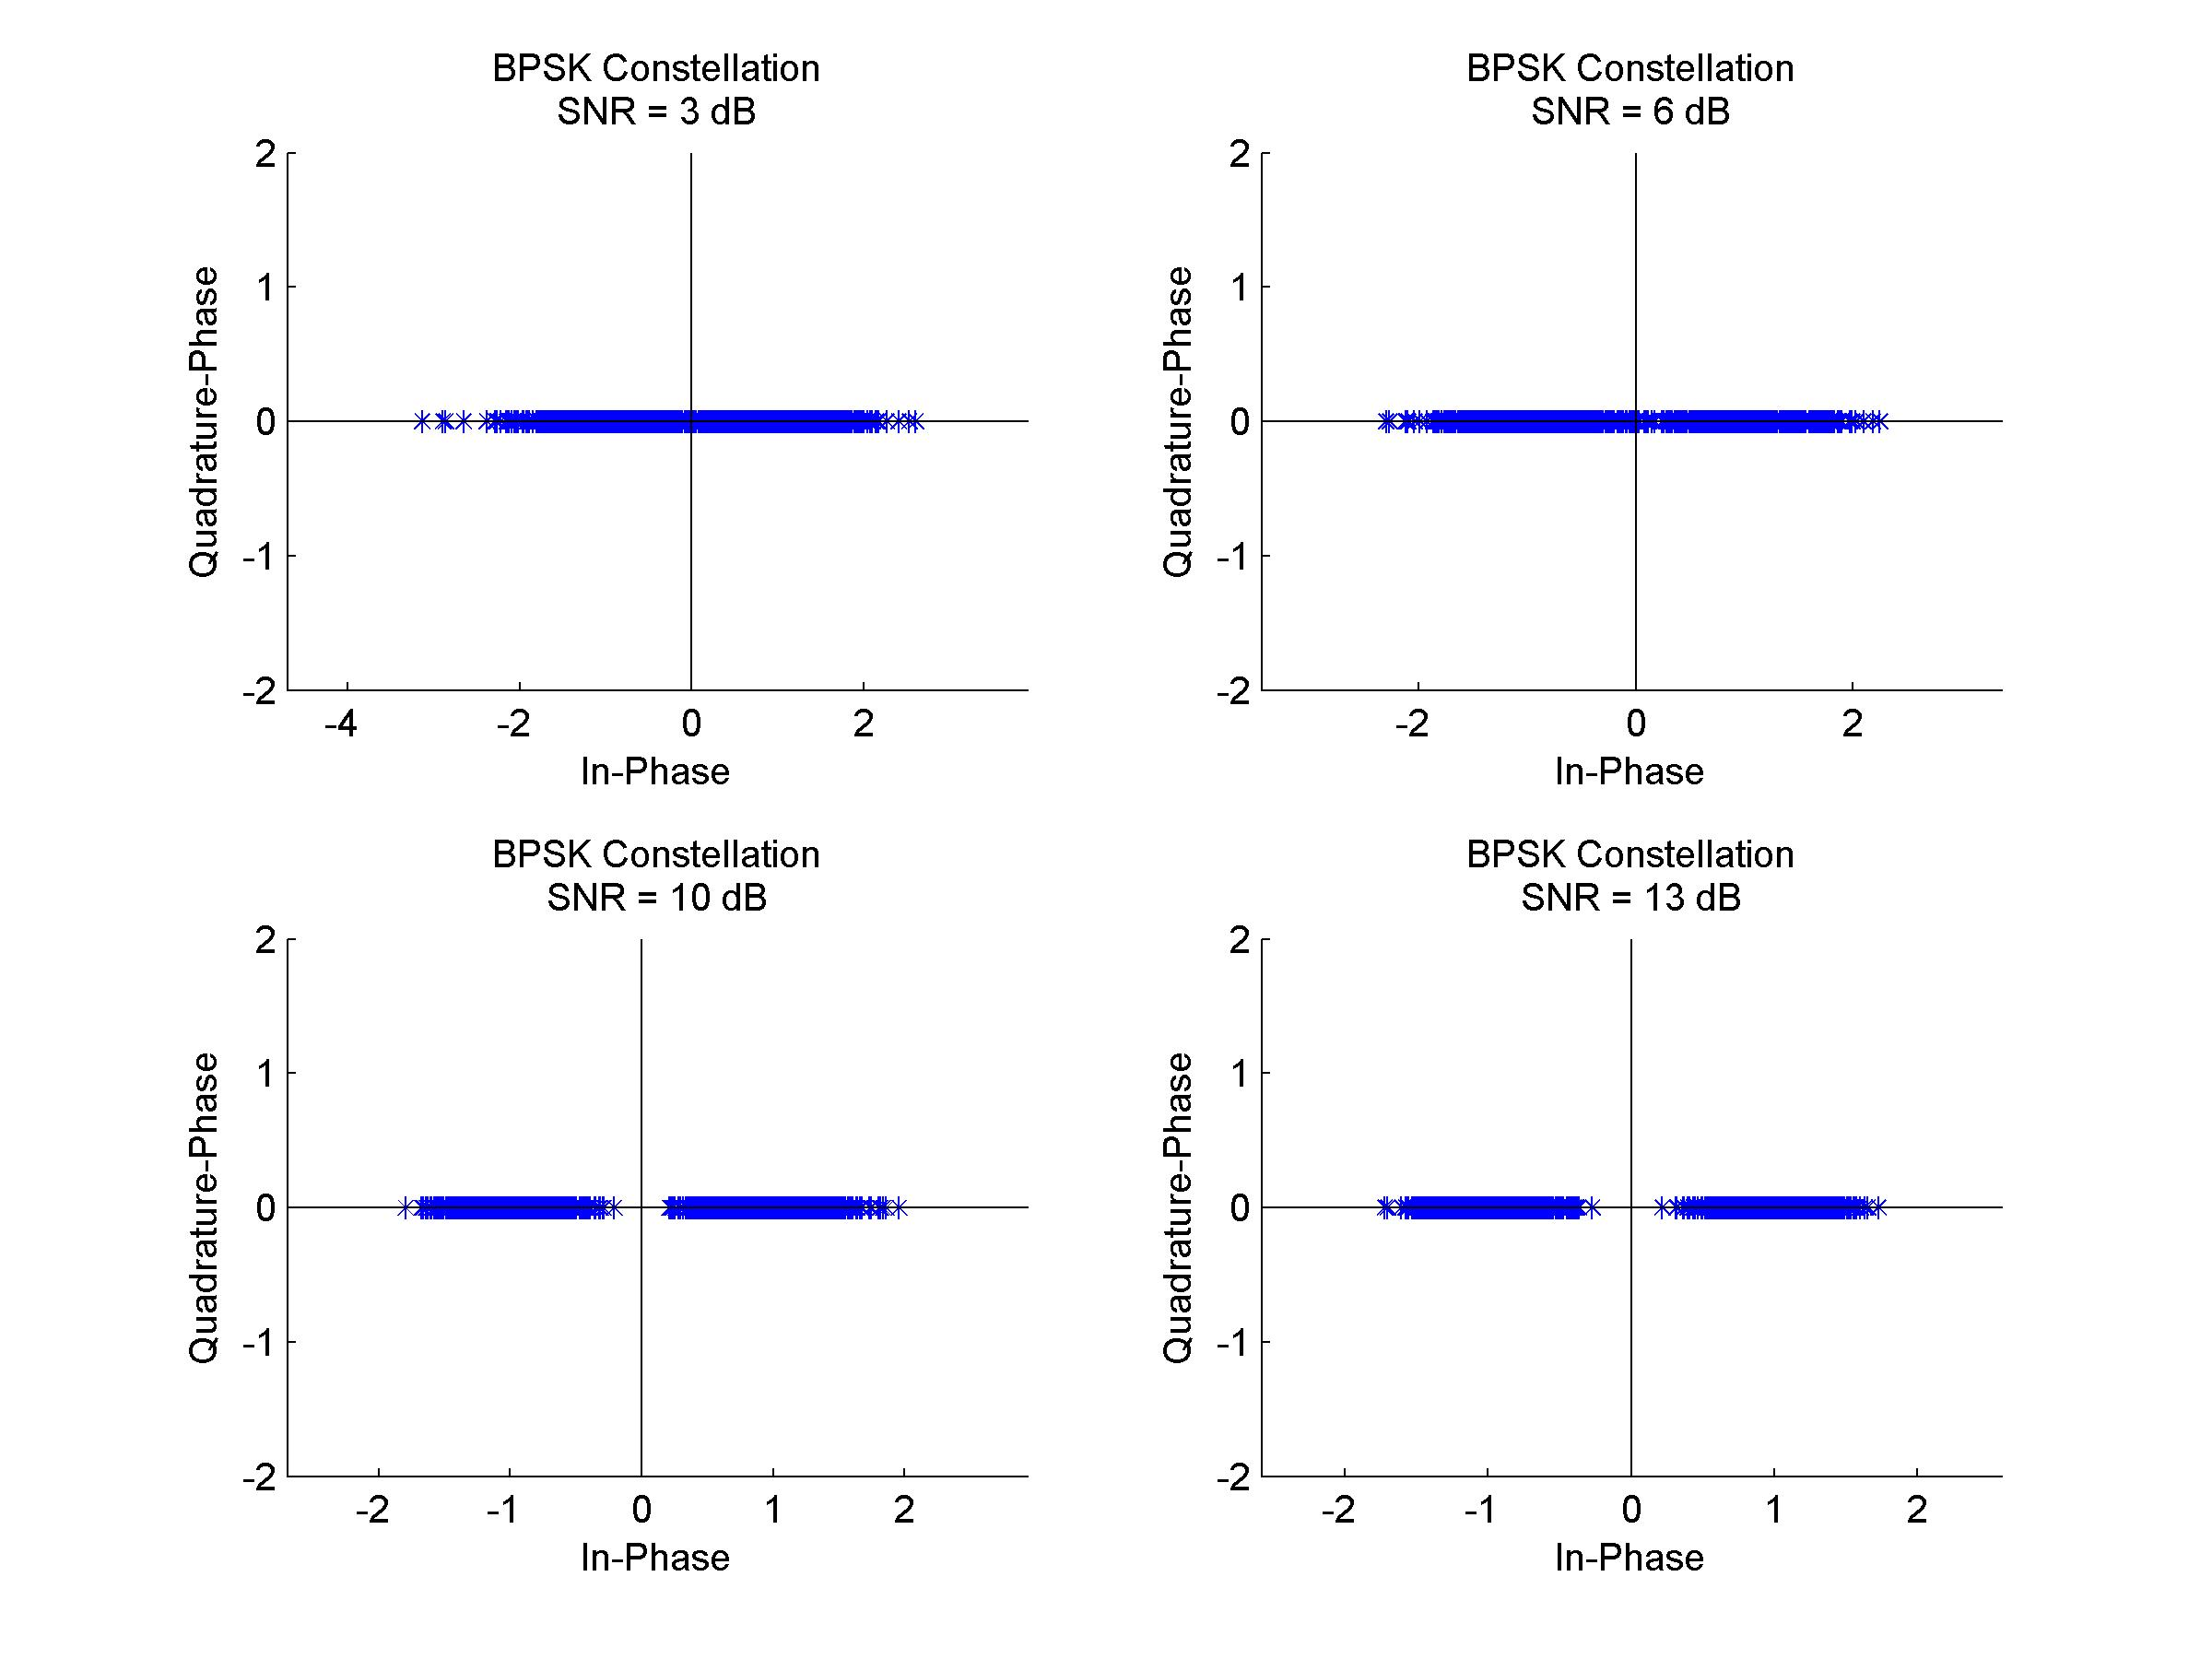
\includegraphics[width=0.7\textwidth]{bpConst1.jpg}
\caption{Constellation plot for a BPSK modulated signal with no equalization under channel reponse $h_1(t)$}
\end{figure}

\begin{figure}[H]
\centering
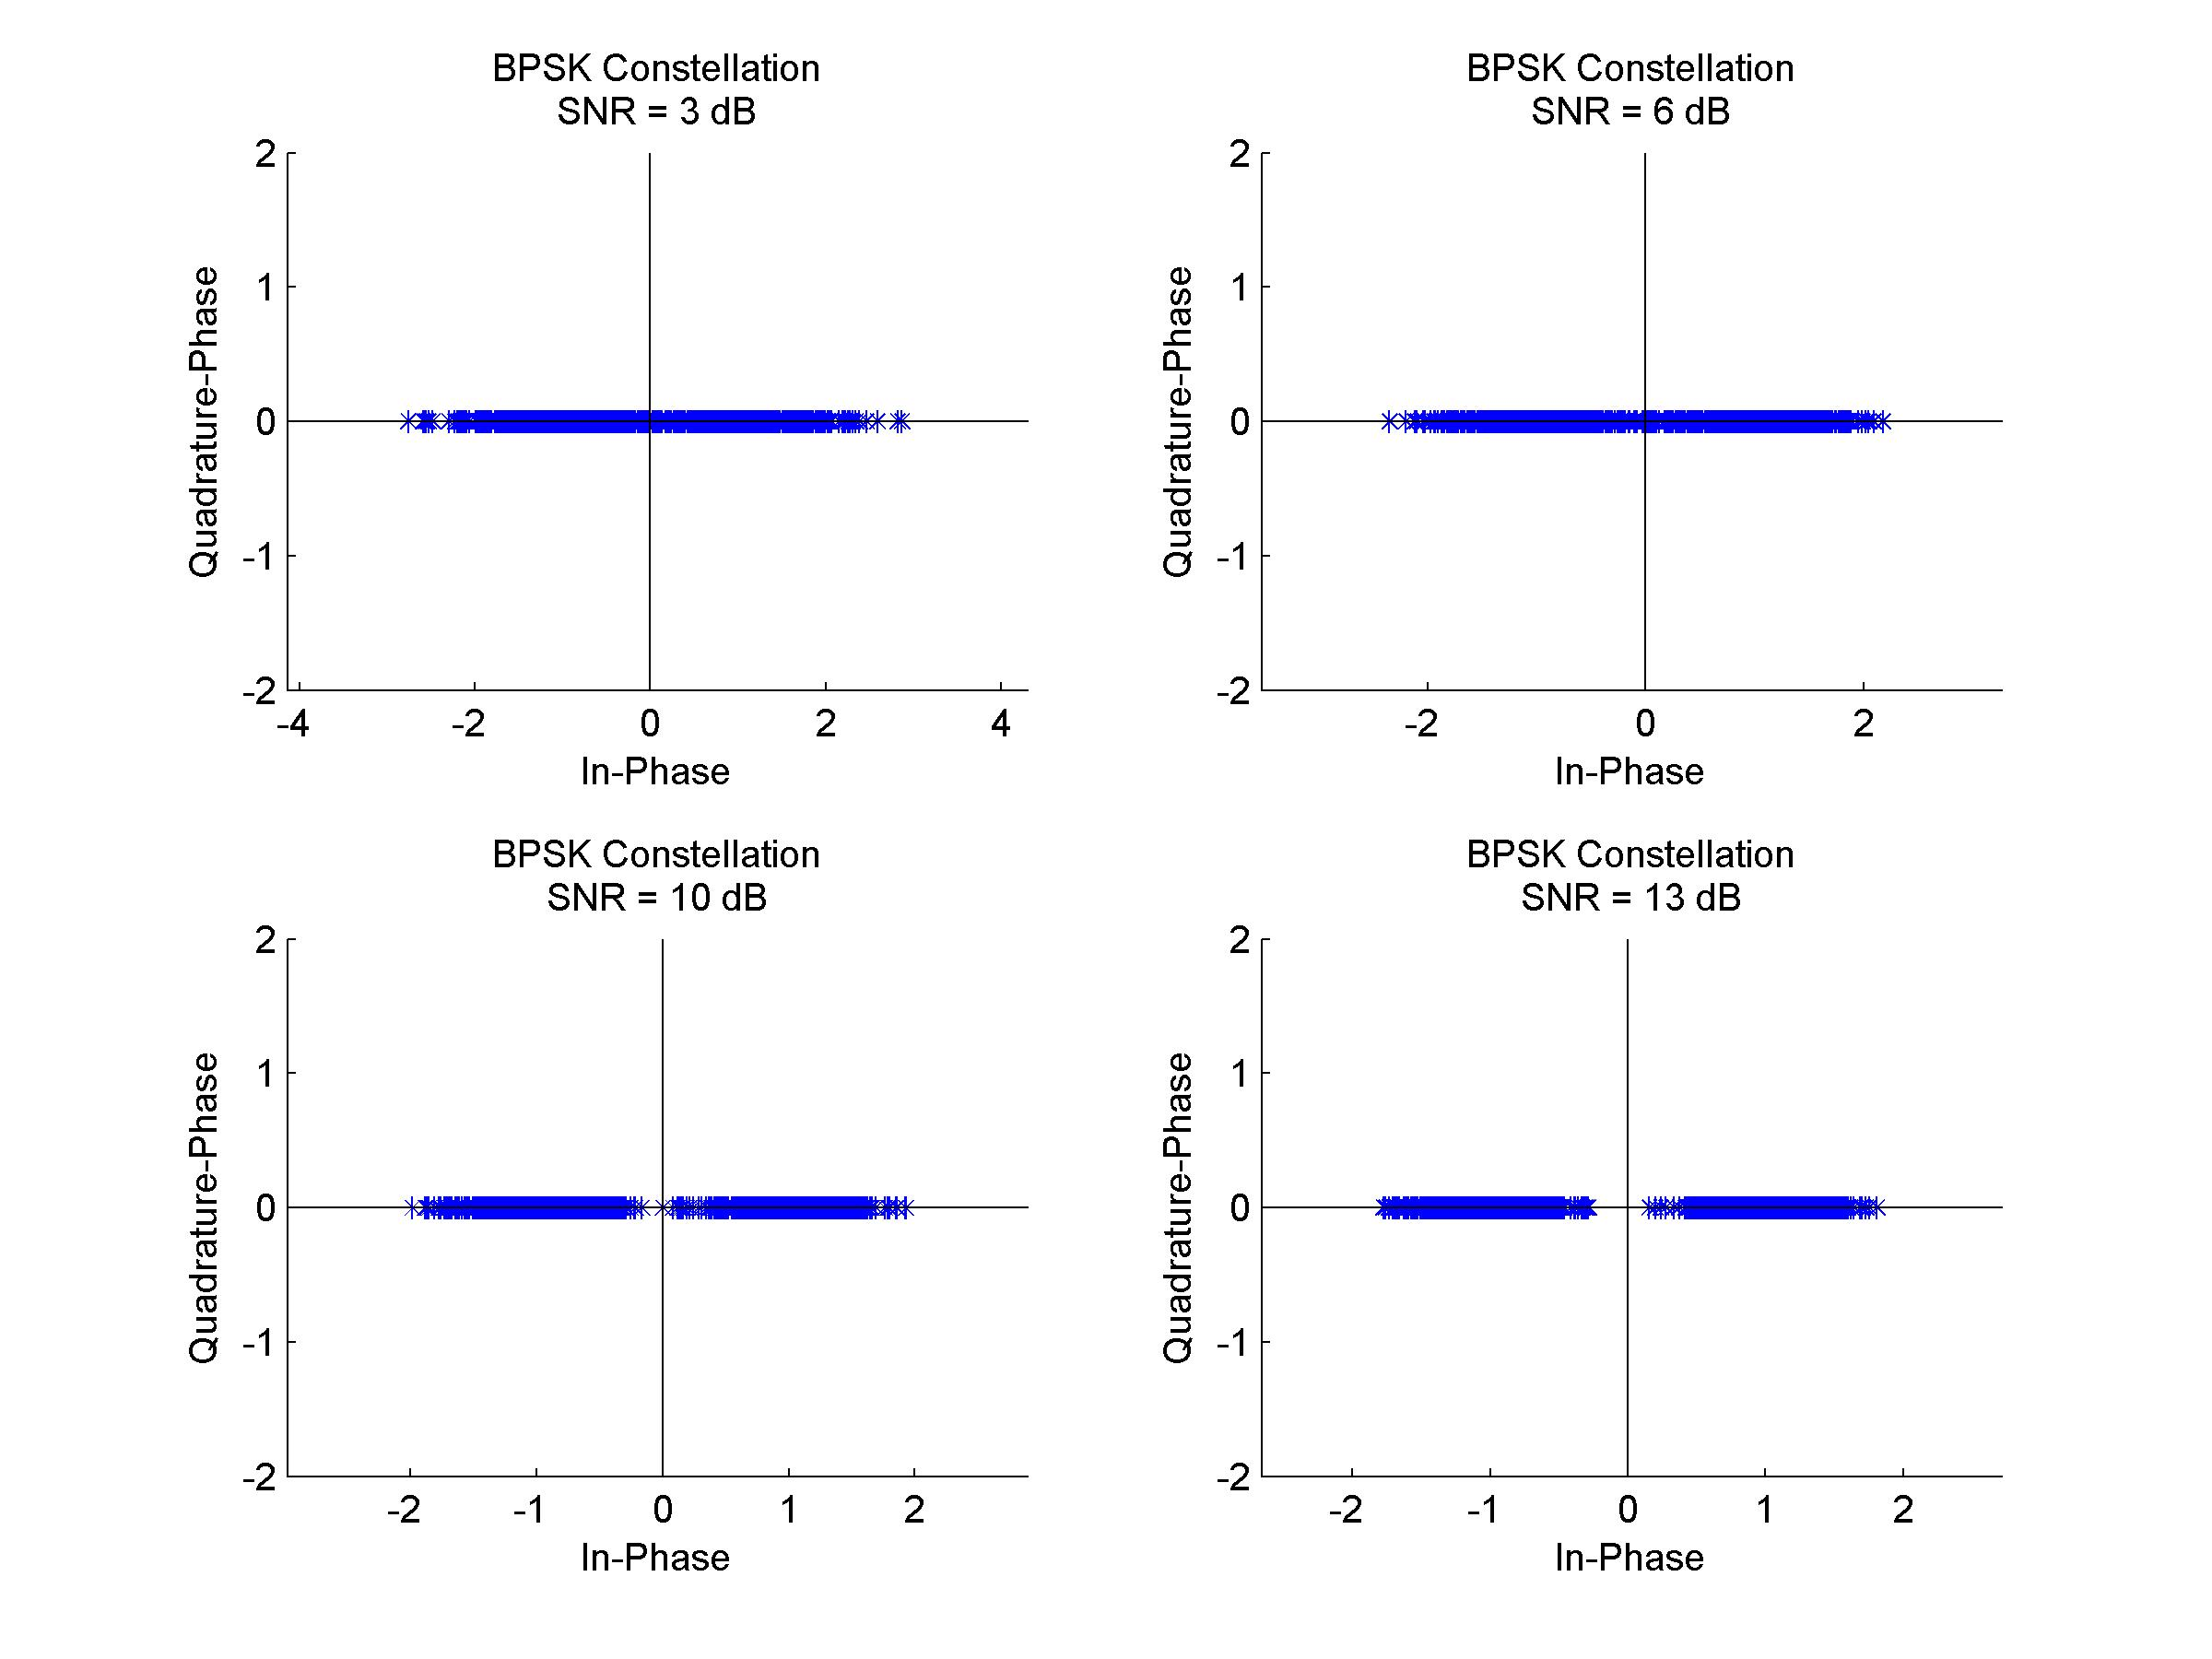
\includegraphics[width=0.7\textwidth]{bpConst2.jpg}
\caption{Constellation plot for a BPSK modulated signal with no equalization under channel reponse $h_2(t)$}
\end{figure}

\begin{figure}[H]
\centering
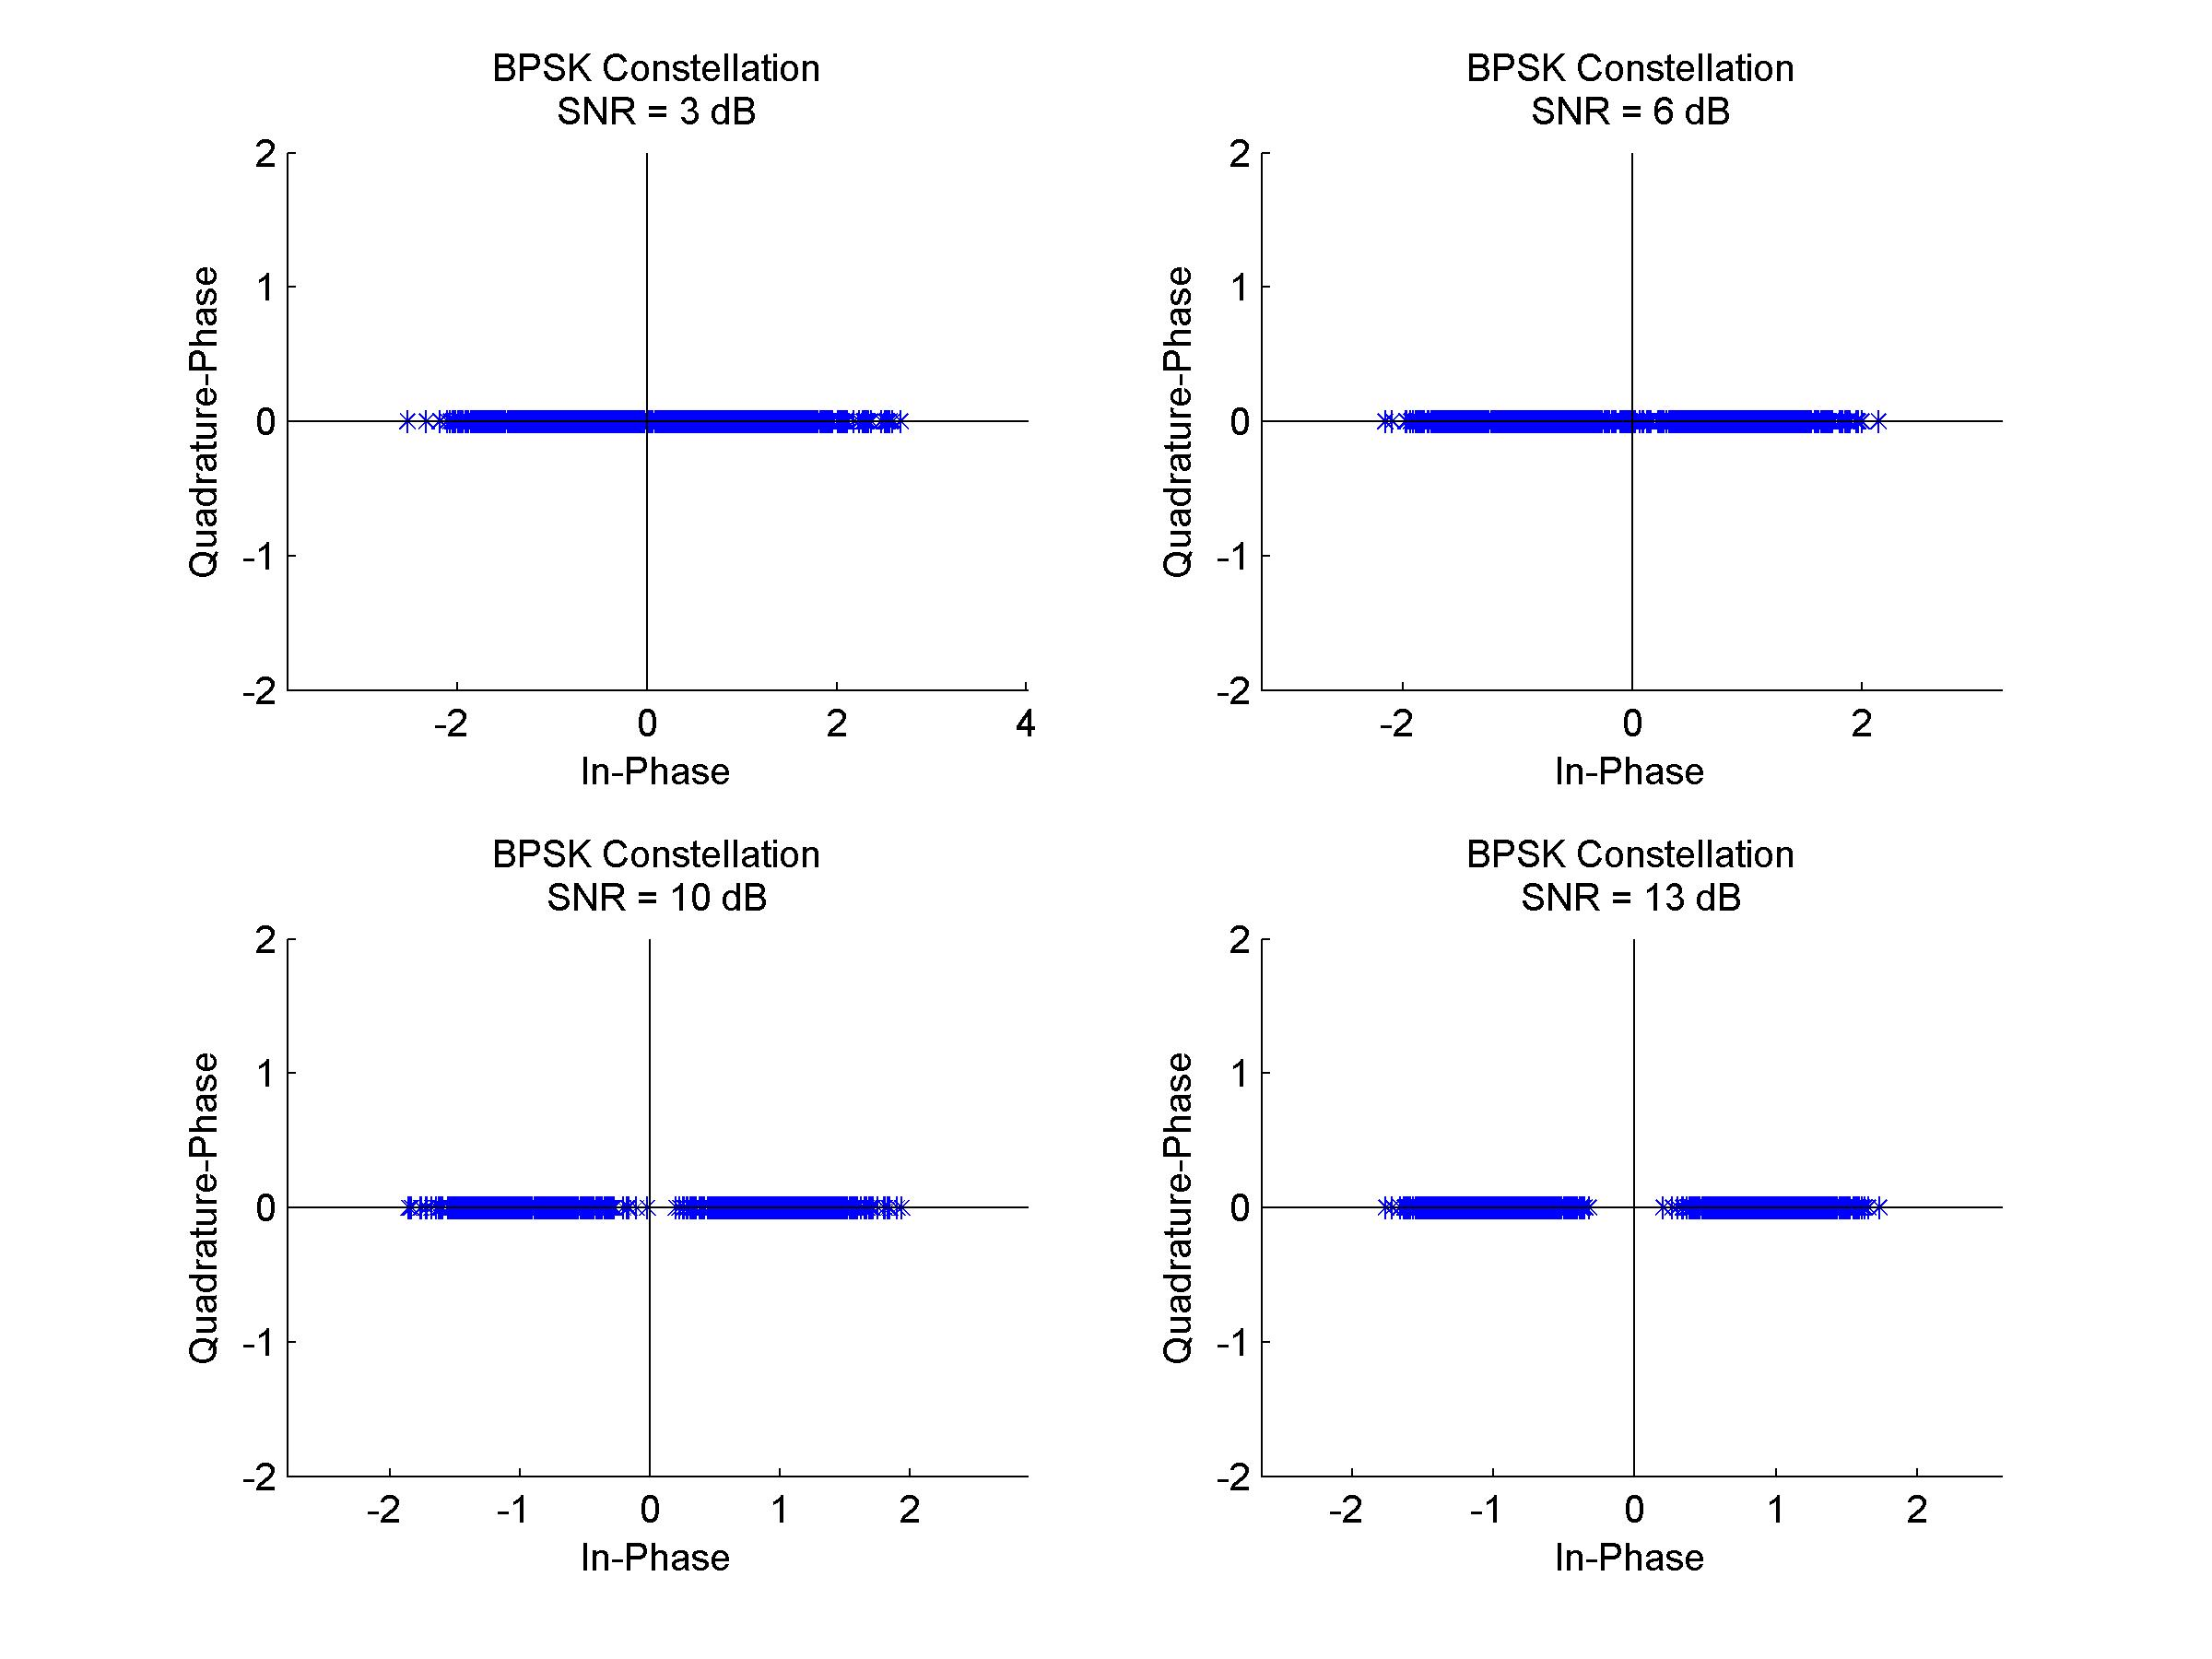
\includegraphics[width=0.7\textwidth]{bpConst3.jpg}
\caption{Constellation plot for a BPSK modulated signal with no equalization under channel reponse $h_3(t)$}
\end{figure}

\subsubsection{BPSK with ZF Equalization}

\begin{figure}[H]
\centering
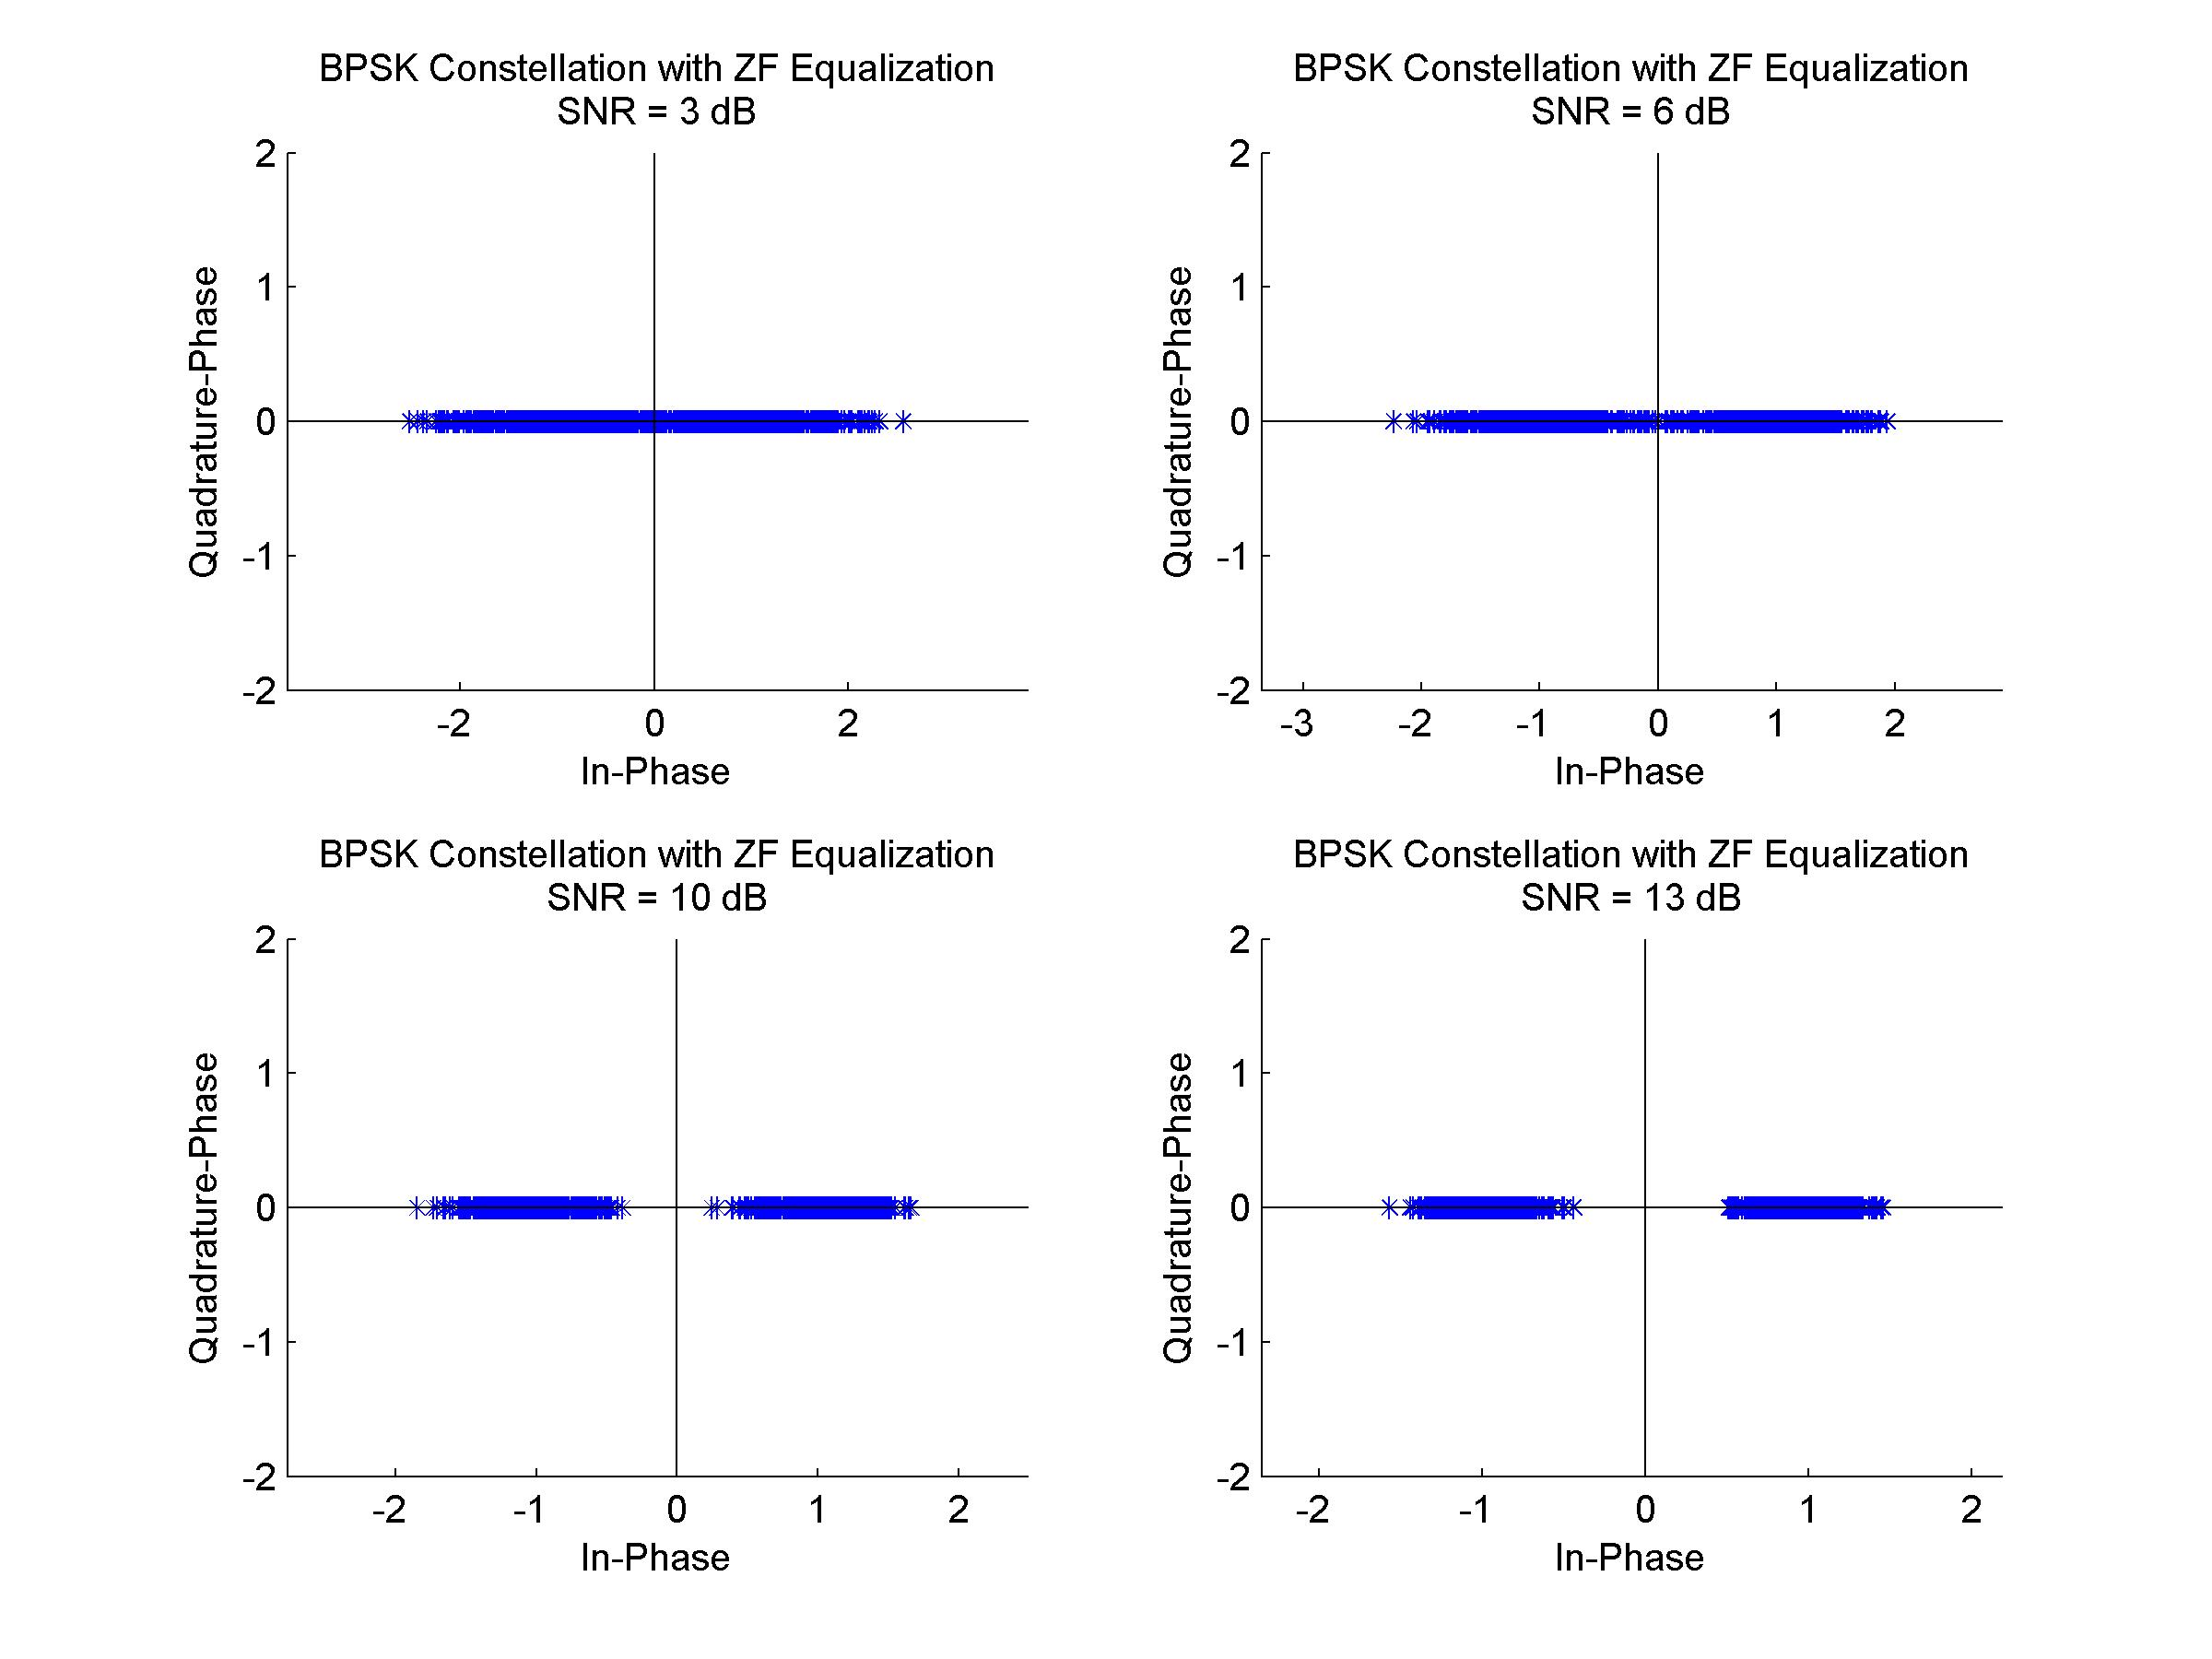
\includegraphics[width=0.7\textwidth]{bpConstZF1.jpg}
\caption{Constellation plot for a BPSK modulated signal with ZF equalization under channel reponse $h_1(t)$}
\end{figure}

\begin{figure}[H]
\centering
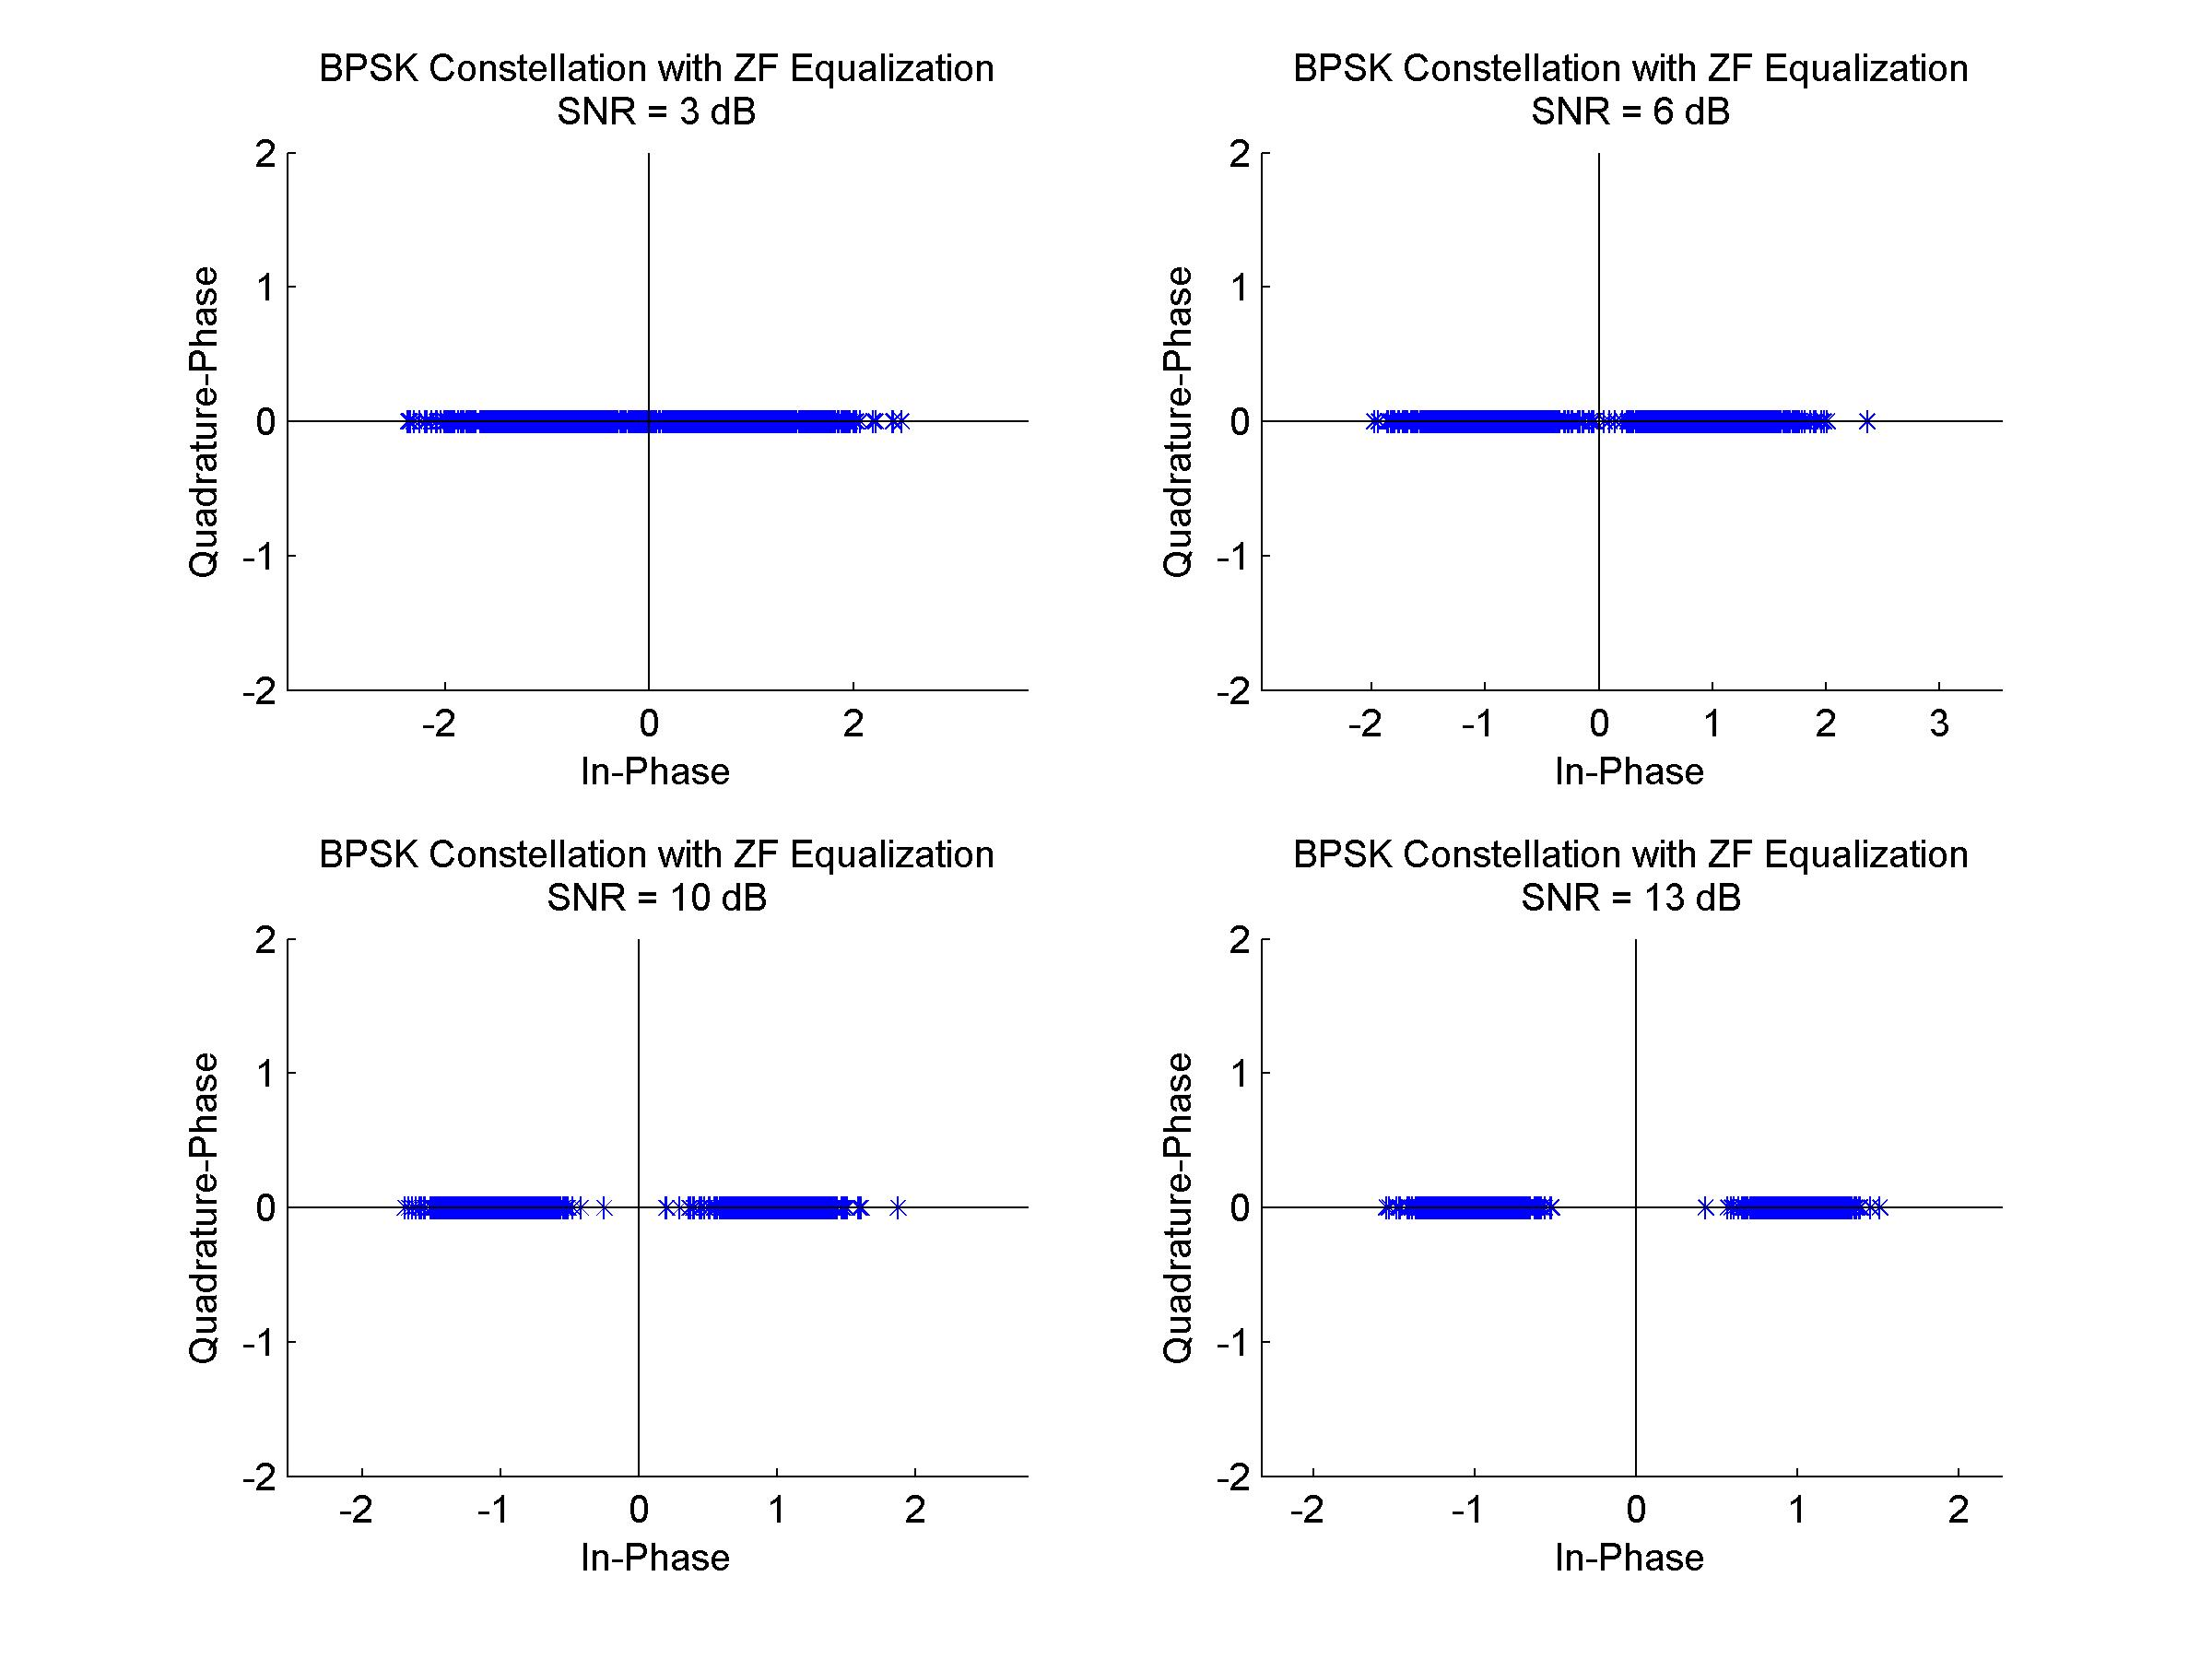
\includegraphics[width=0.7\textwidth]{bpConstZF2.jpg}
\caption{Constellation plot for a BPSK modulated signal with ZF equalization under channel reponse $h_2(t)$}
\end{figure}

\begin{figure}[H]
\centering
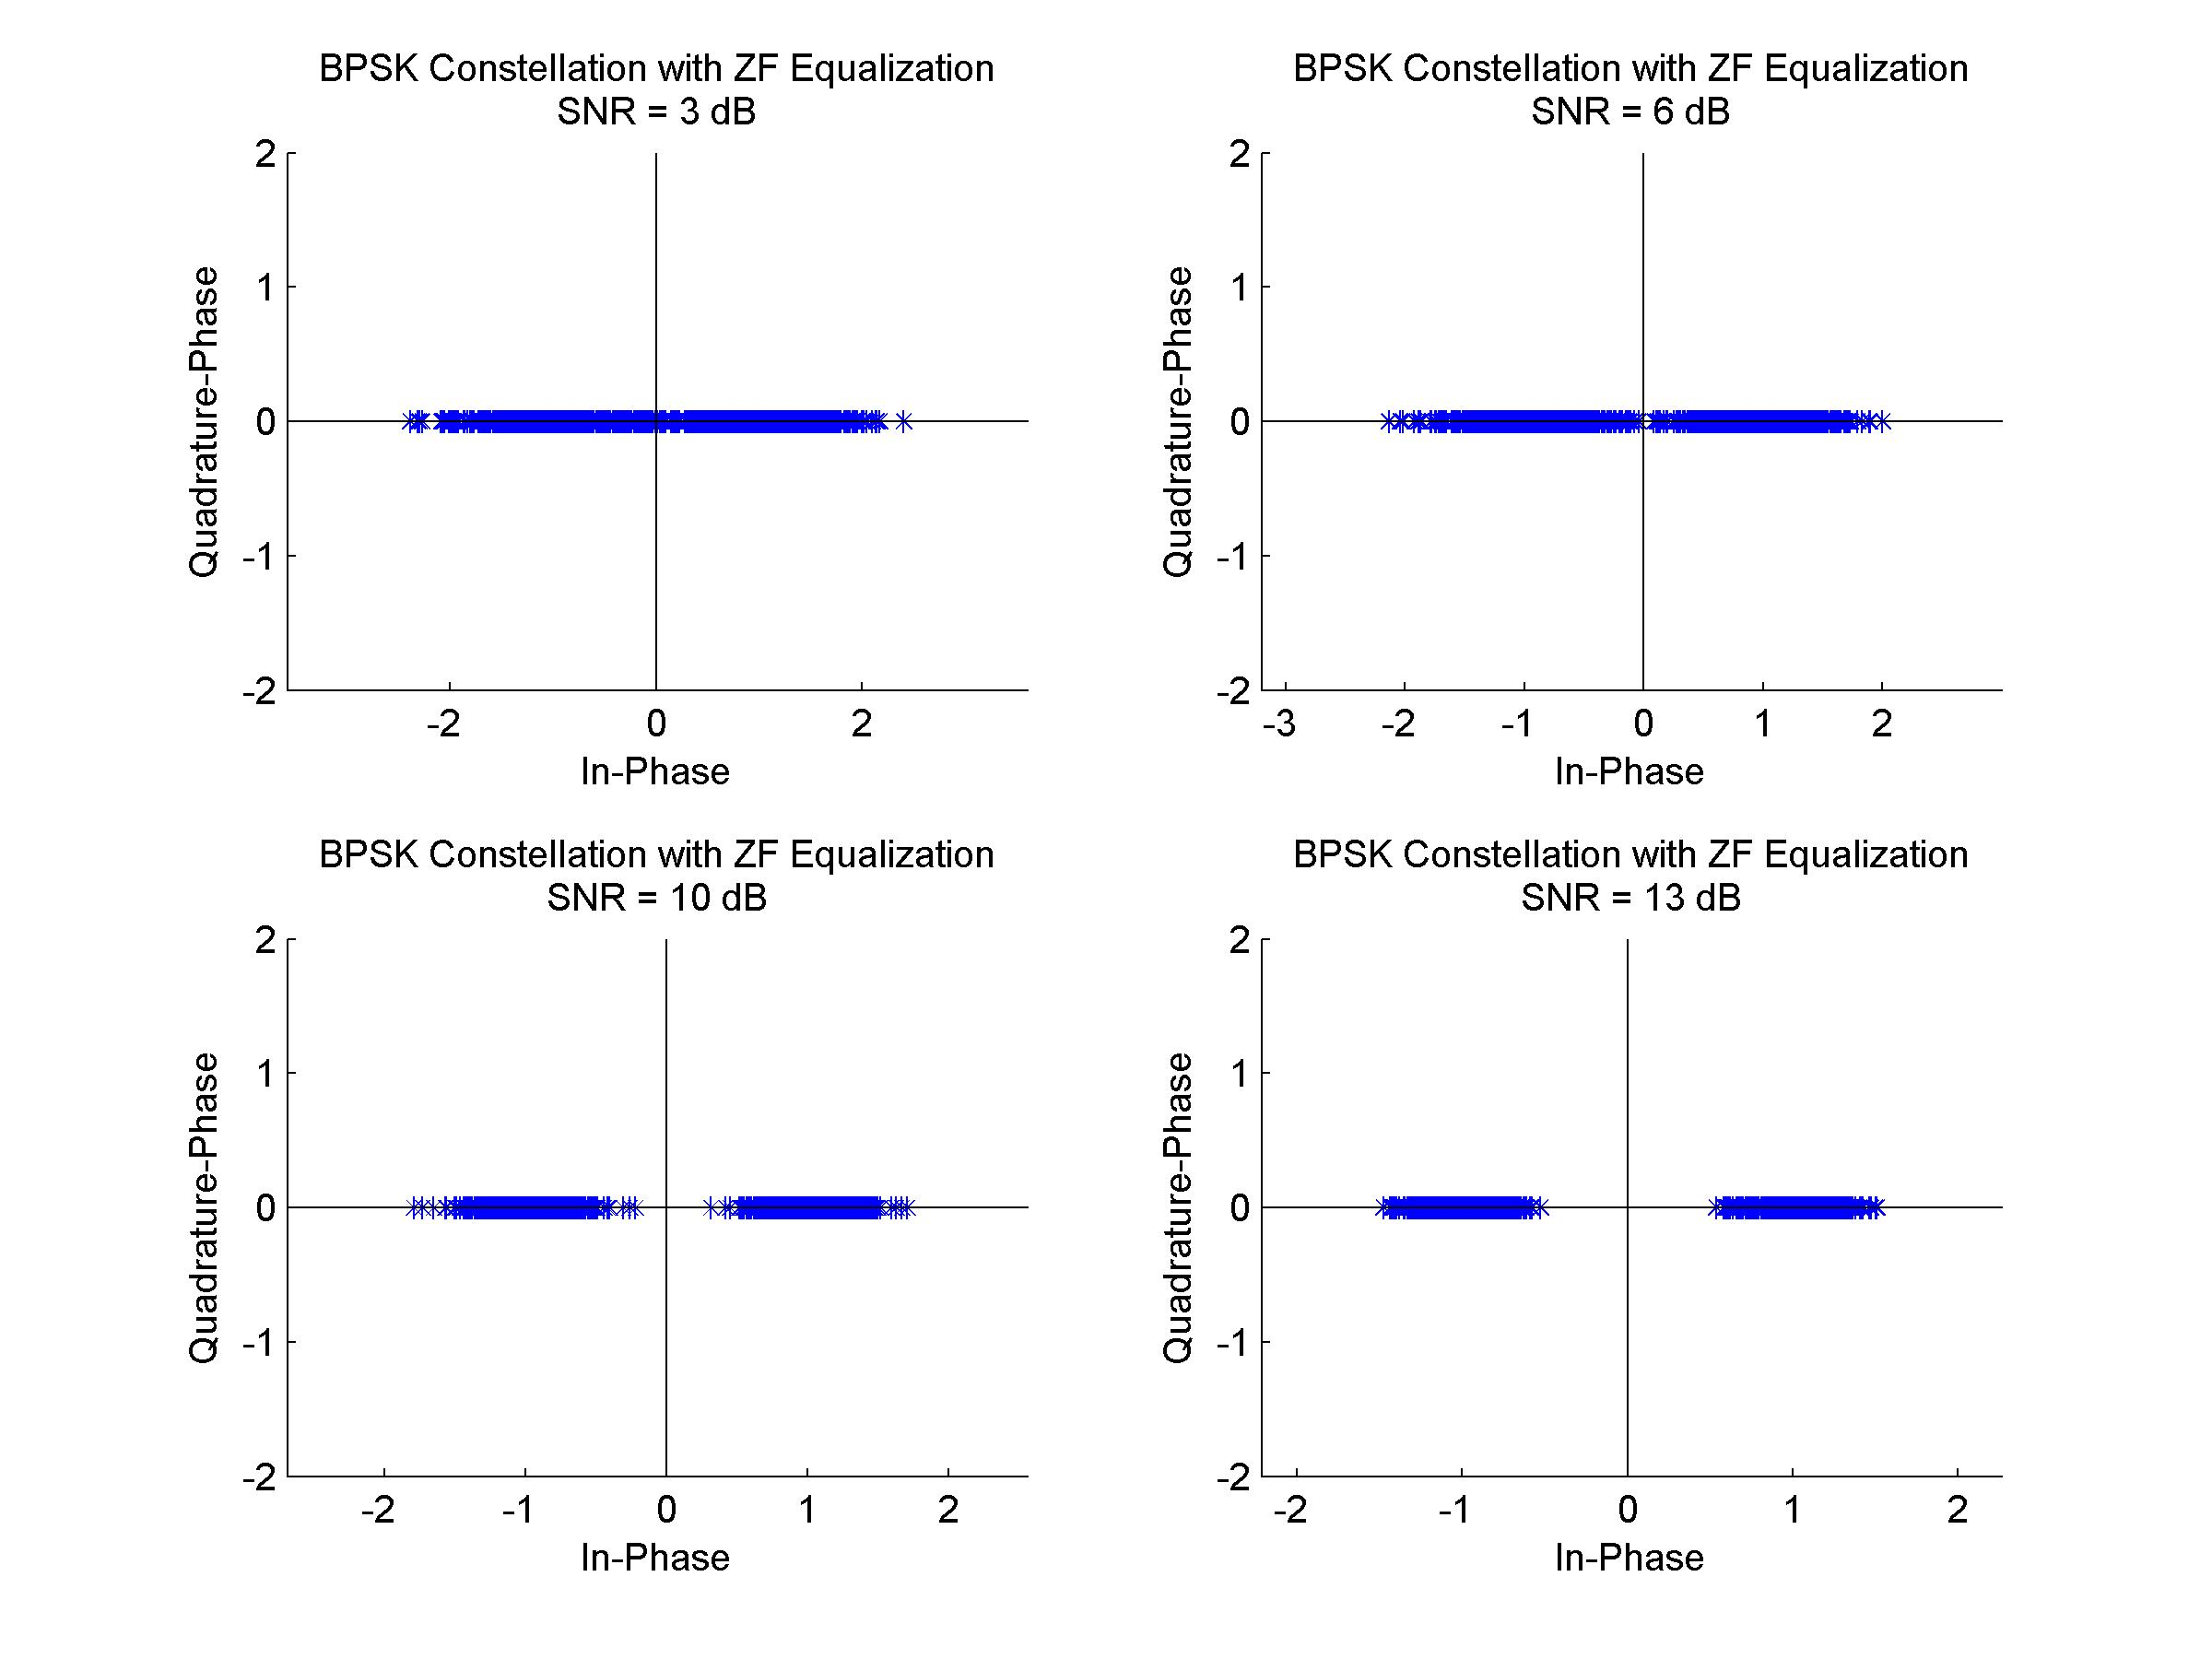
\includegraphics[width=0.7\textwidth]{bpConstZF3.jpg}
\caption{Constellation plot for a BPSK modulated signal with ZF equalization under channel reponse $h_3(t)$}
\end{figure}

\subsubsection{BPSK with MMSE Equalization}

\begin{figure}[H]
\centering
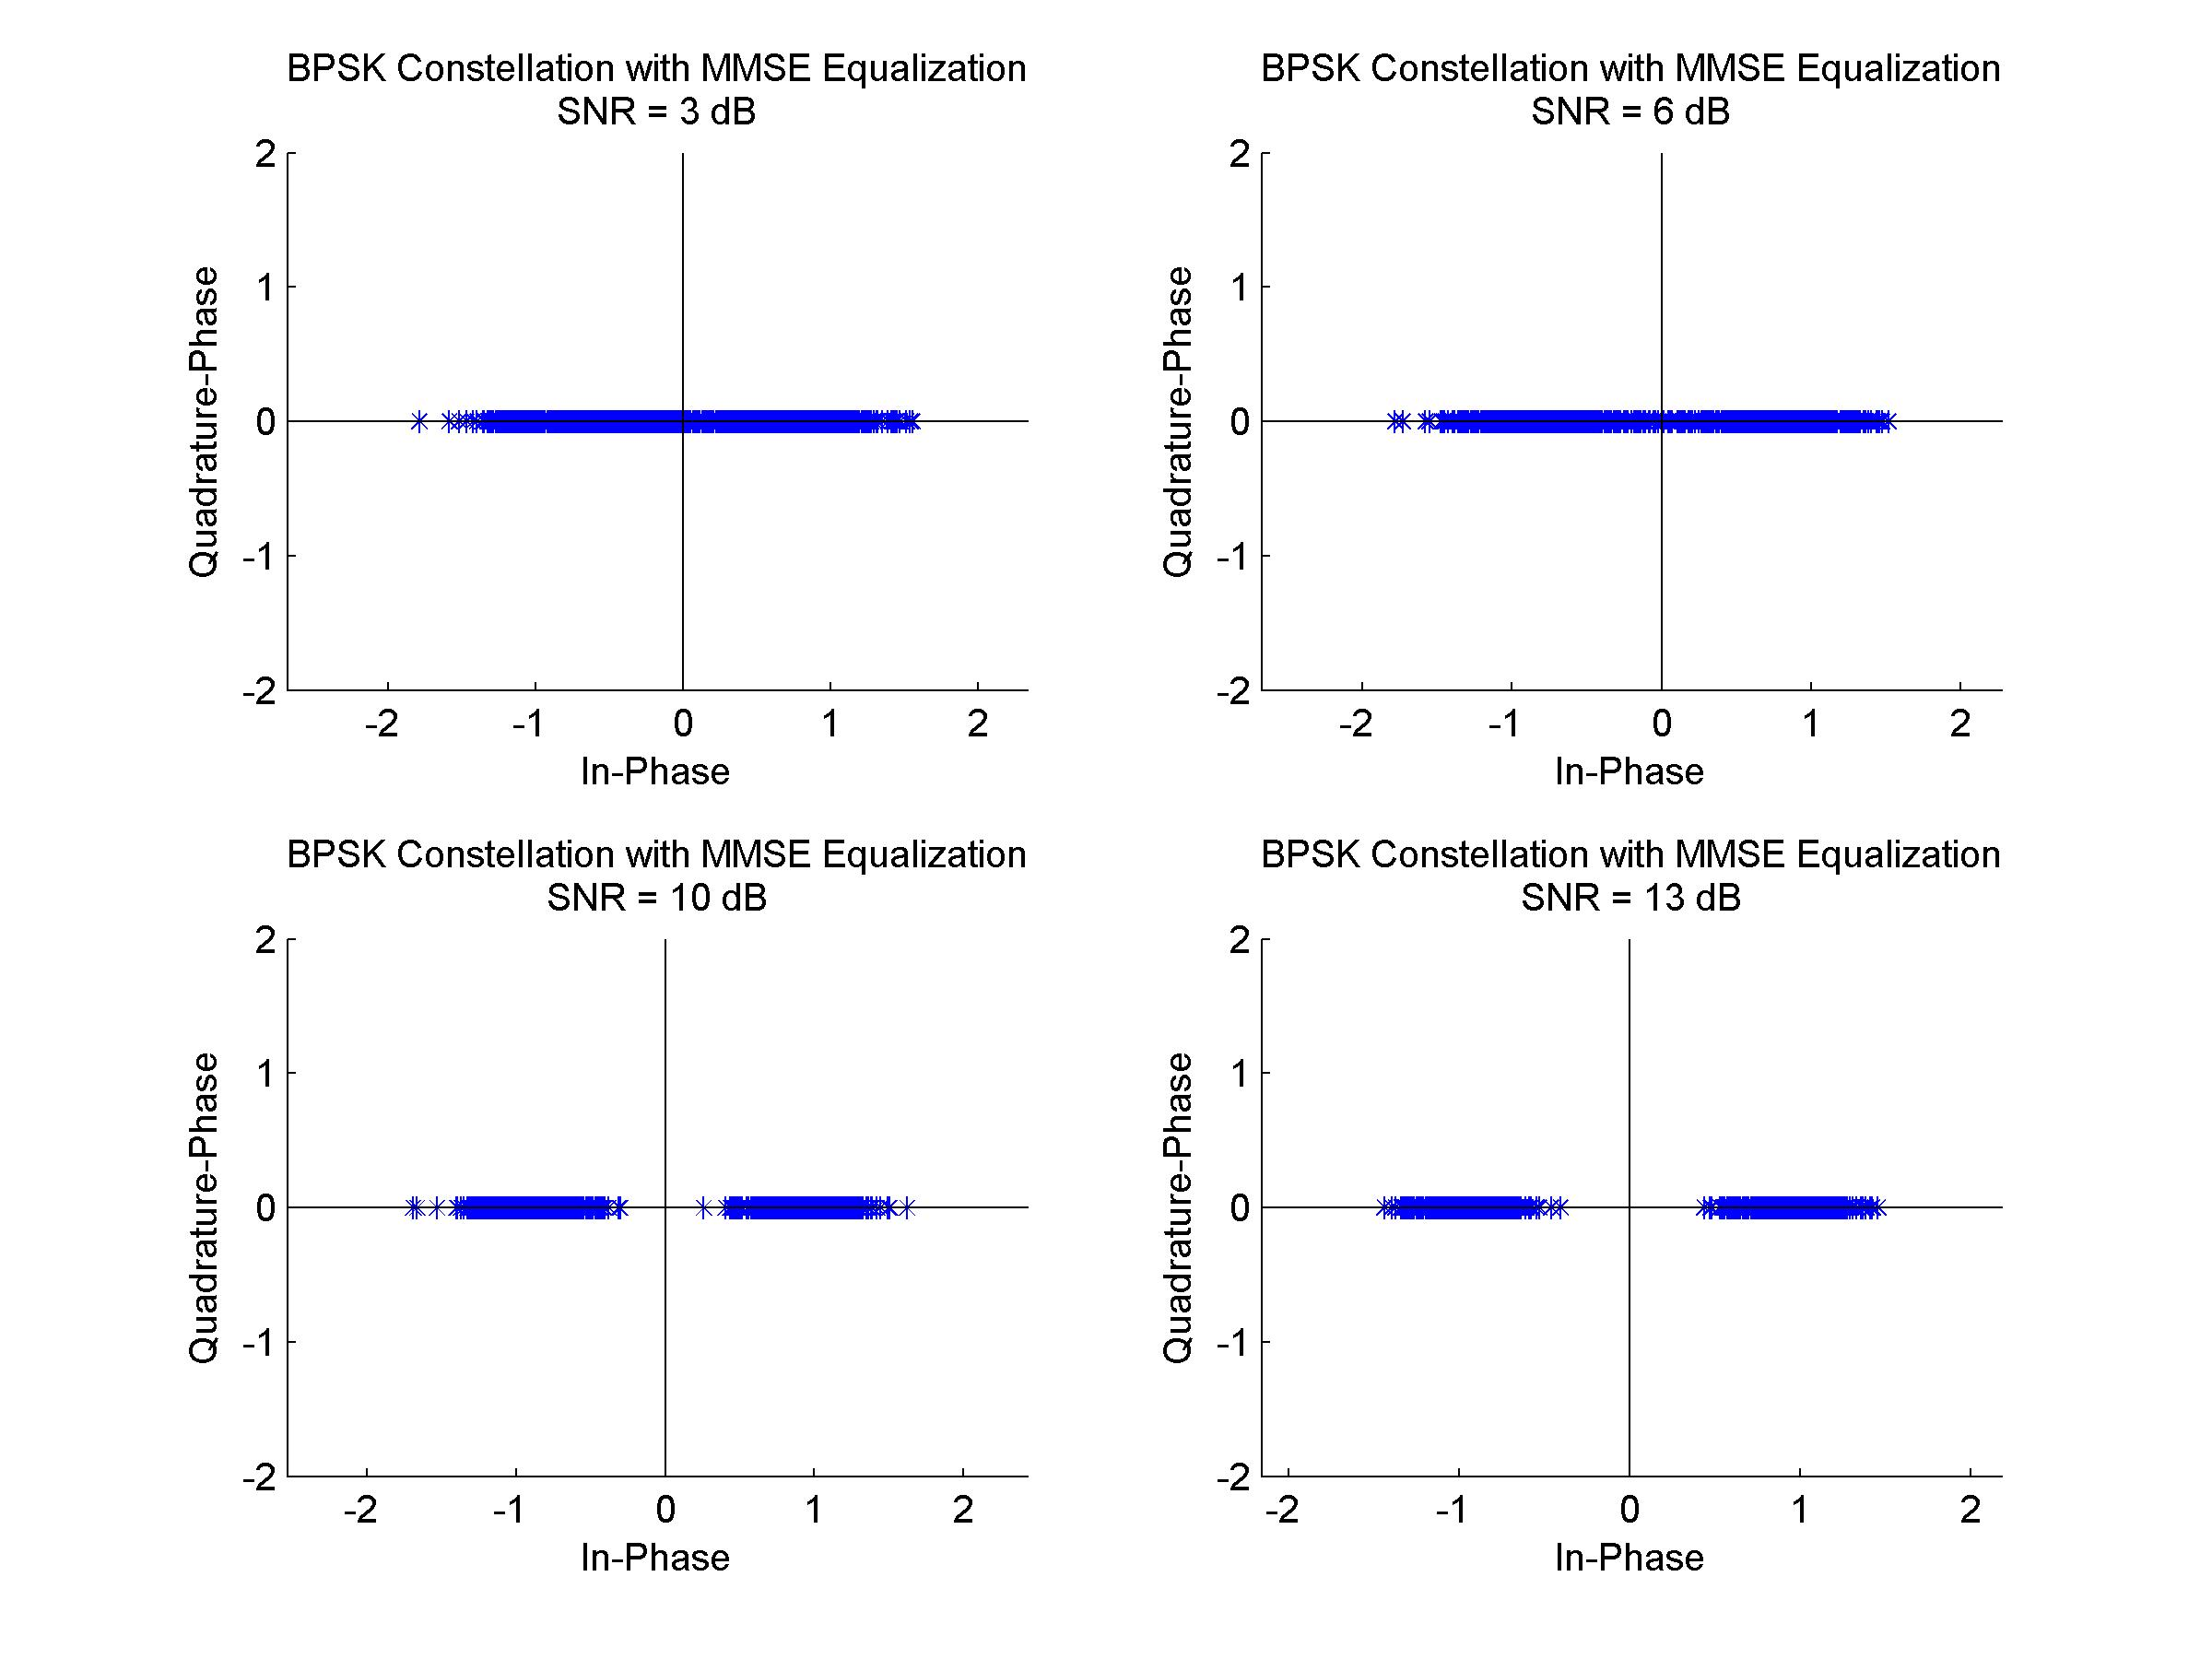
\includegraphics[width=0.7\textwidth]{bpConstMMSE1.jpg}
\caption{Constellation plot for a BPSK modulated signal with MMSE equalization under channel reponse $h_1(t)$}
\end{figure}

\begin{figure}[H]
\centering
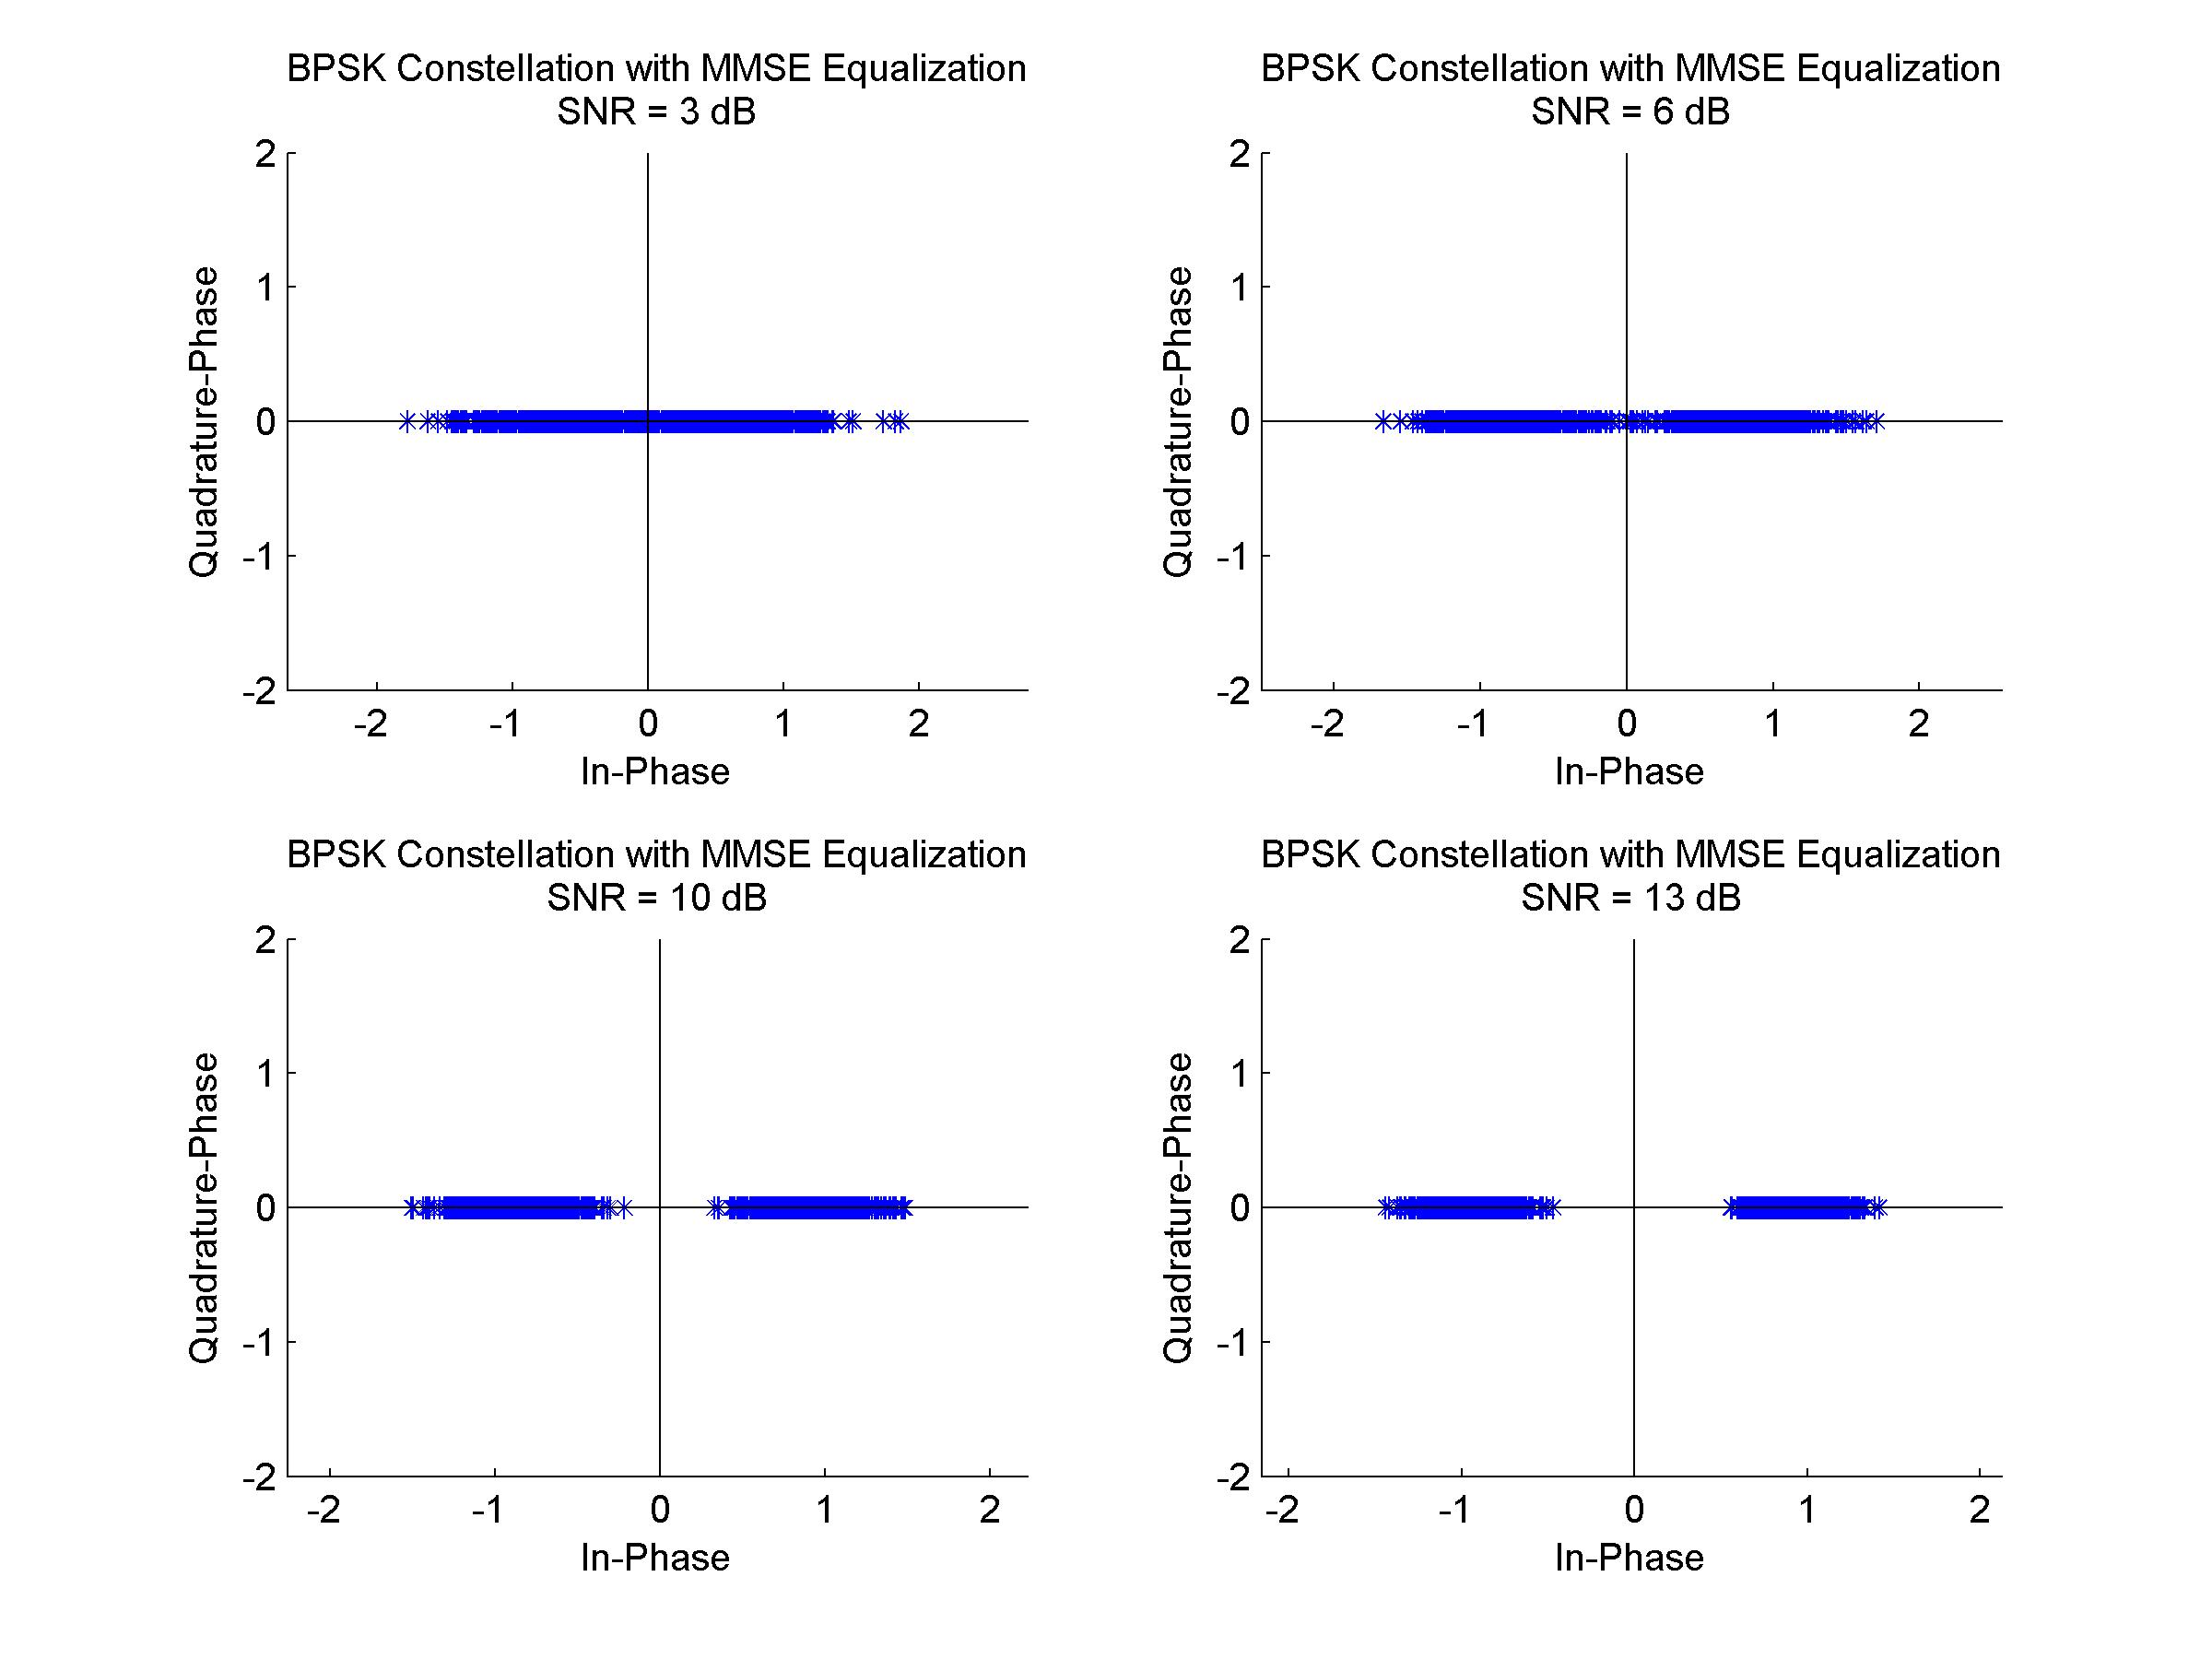
\includegraphics[width=0.7\textwidth]{bpConstMMSE2.jpg}
\caption{Constellation plot for a BPSK modulated signal with MMSE equalization under channel reponse $h_2(t)$}
\end{figure}

\begin{figure}[H]
\centering
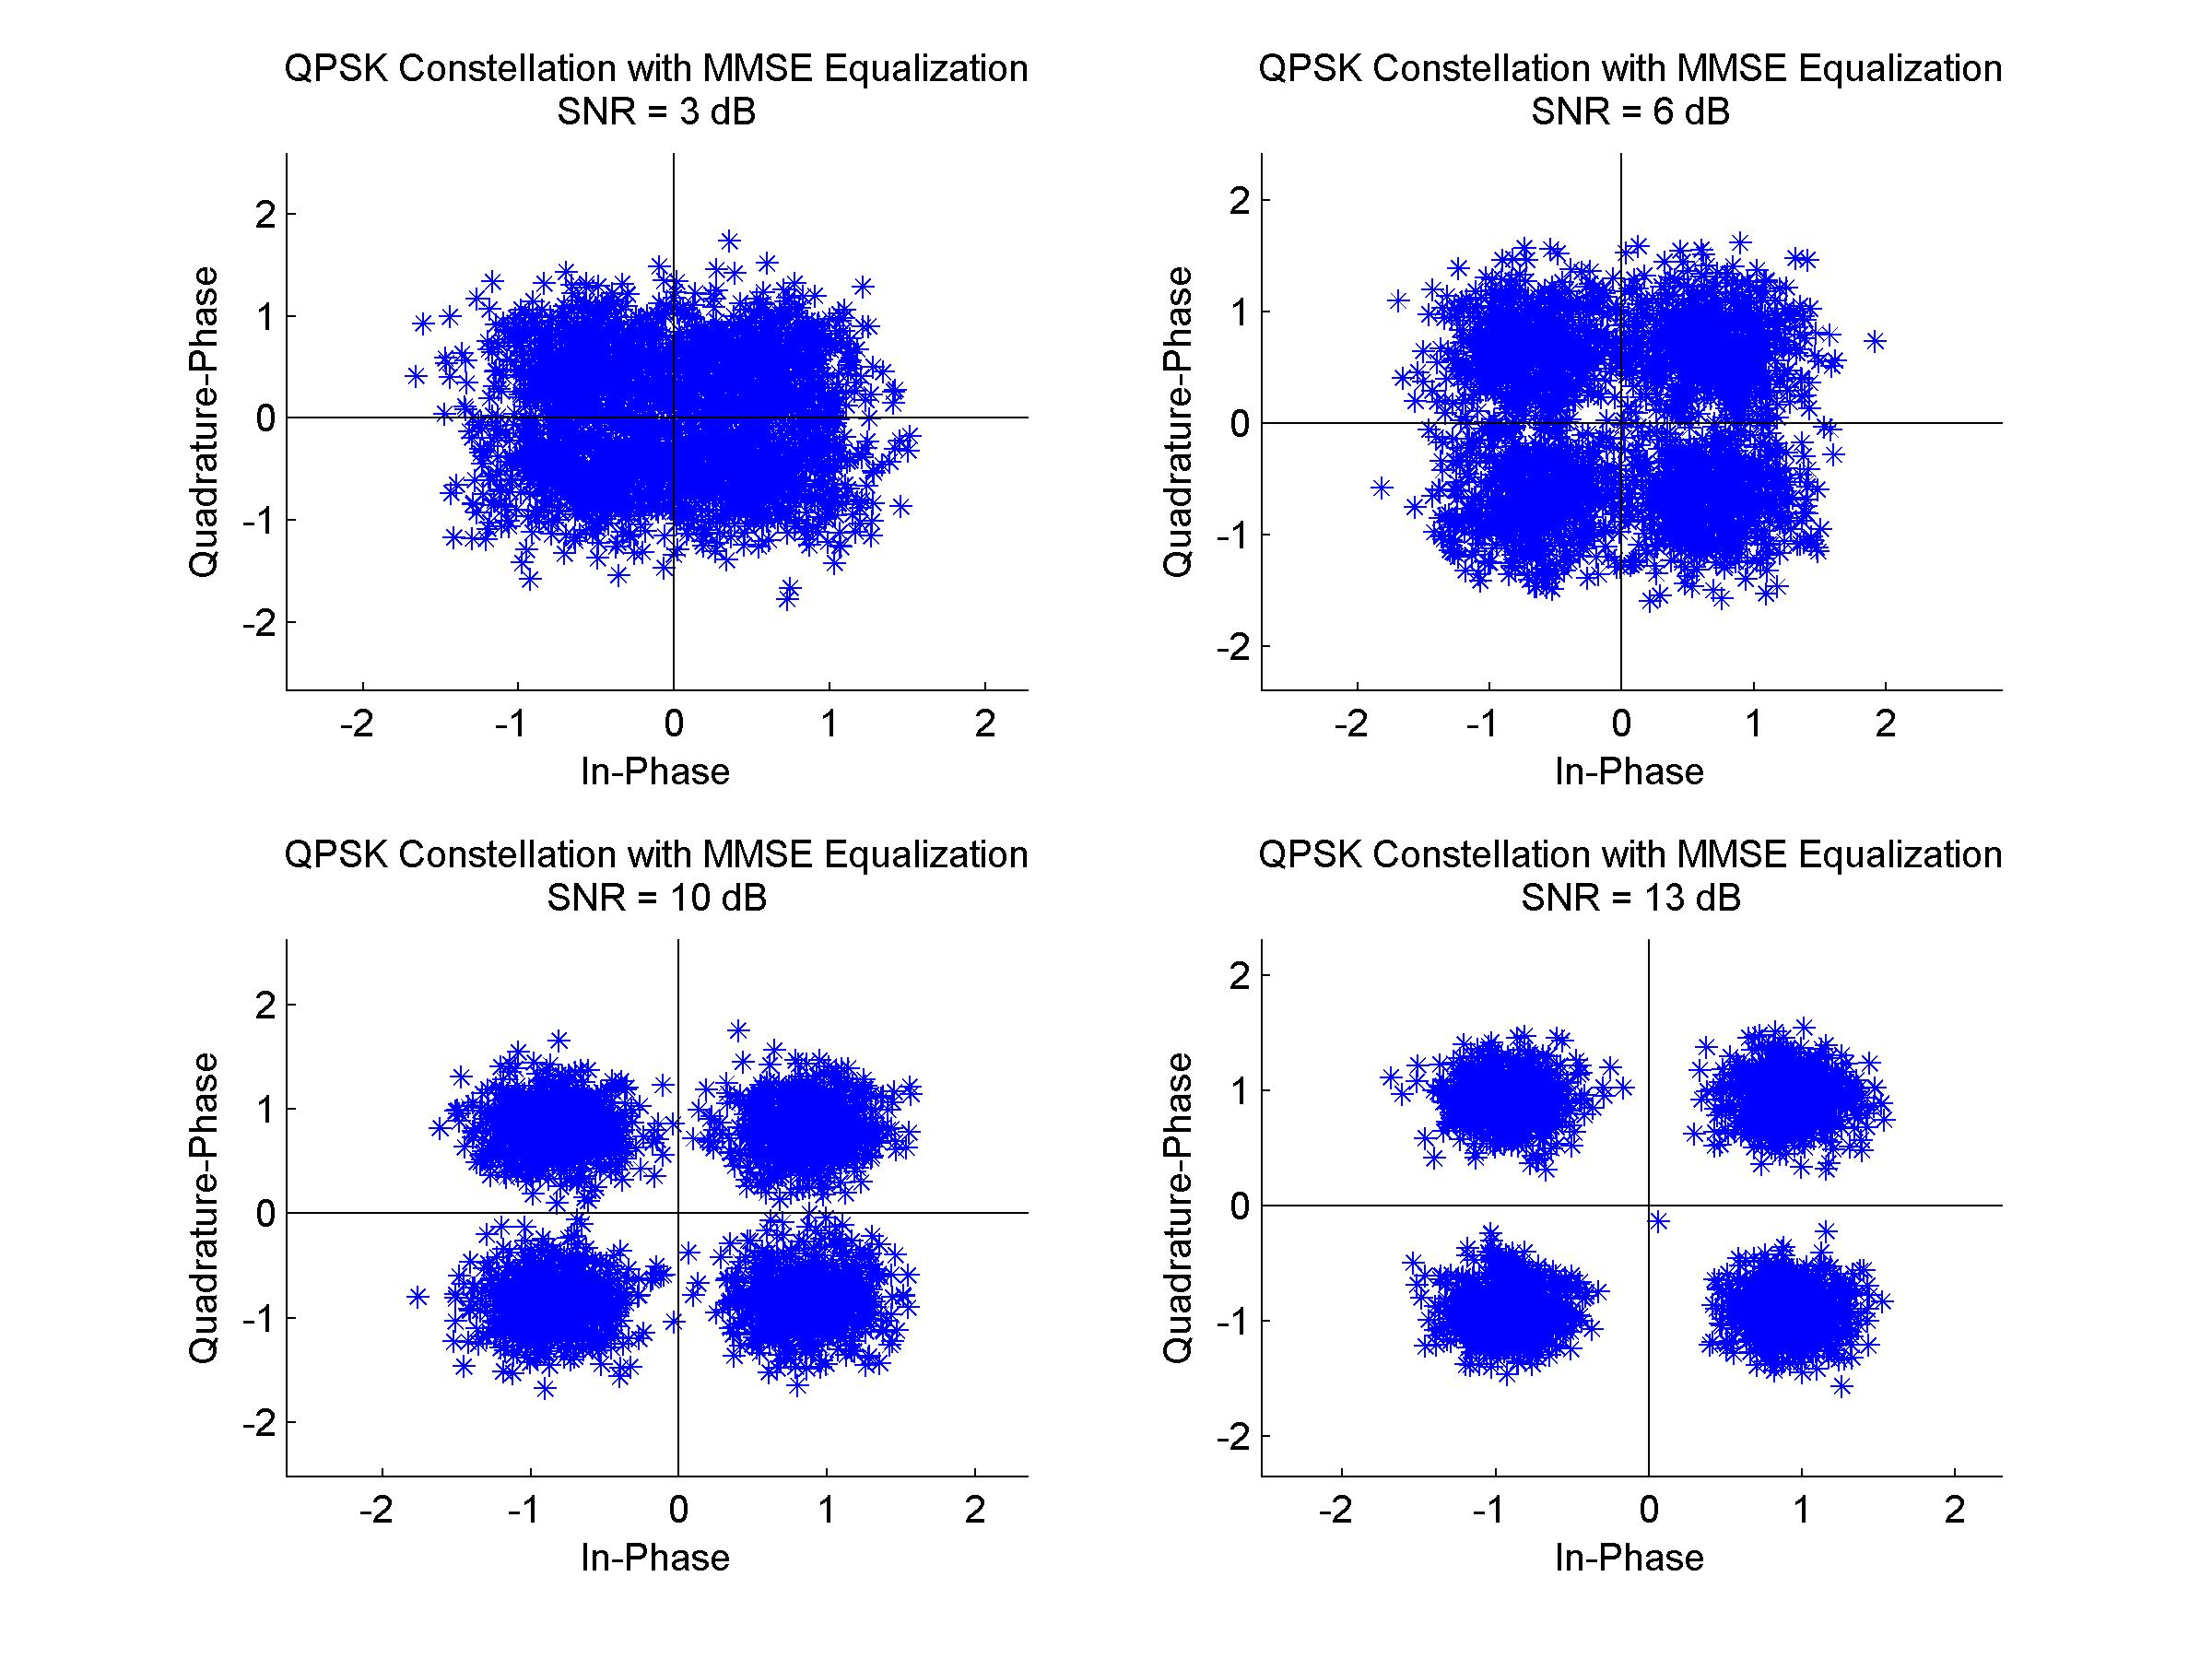
\includegraphics[width=0.7\textwidth]{qpConstMMSE3.jpg}
\caption{Constellation plot for a BPSK modulated signal with MMSE equalization under channel reponse $h_3(t)$}
\end{figure}

\subsubsection{BPSK with MMSE-DFE Equalization}

\begin{figure}[H]
\centering
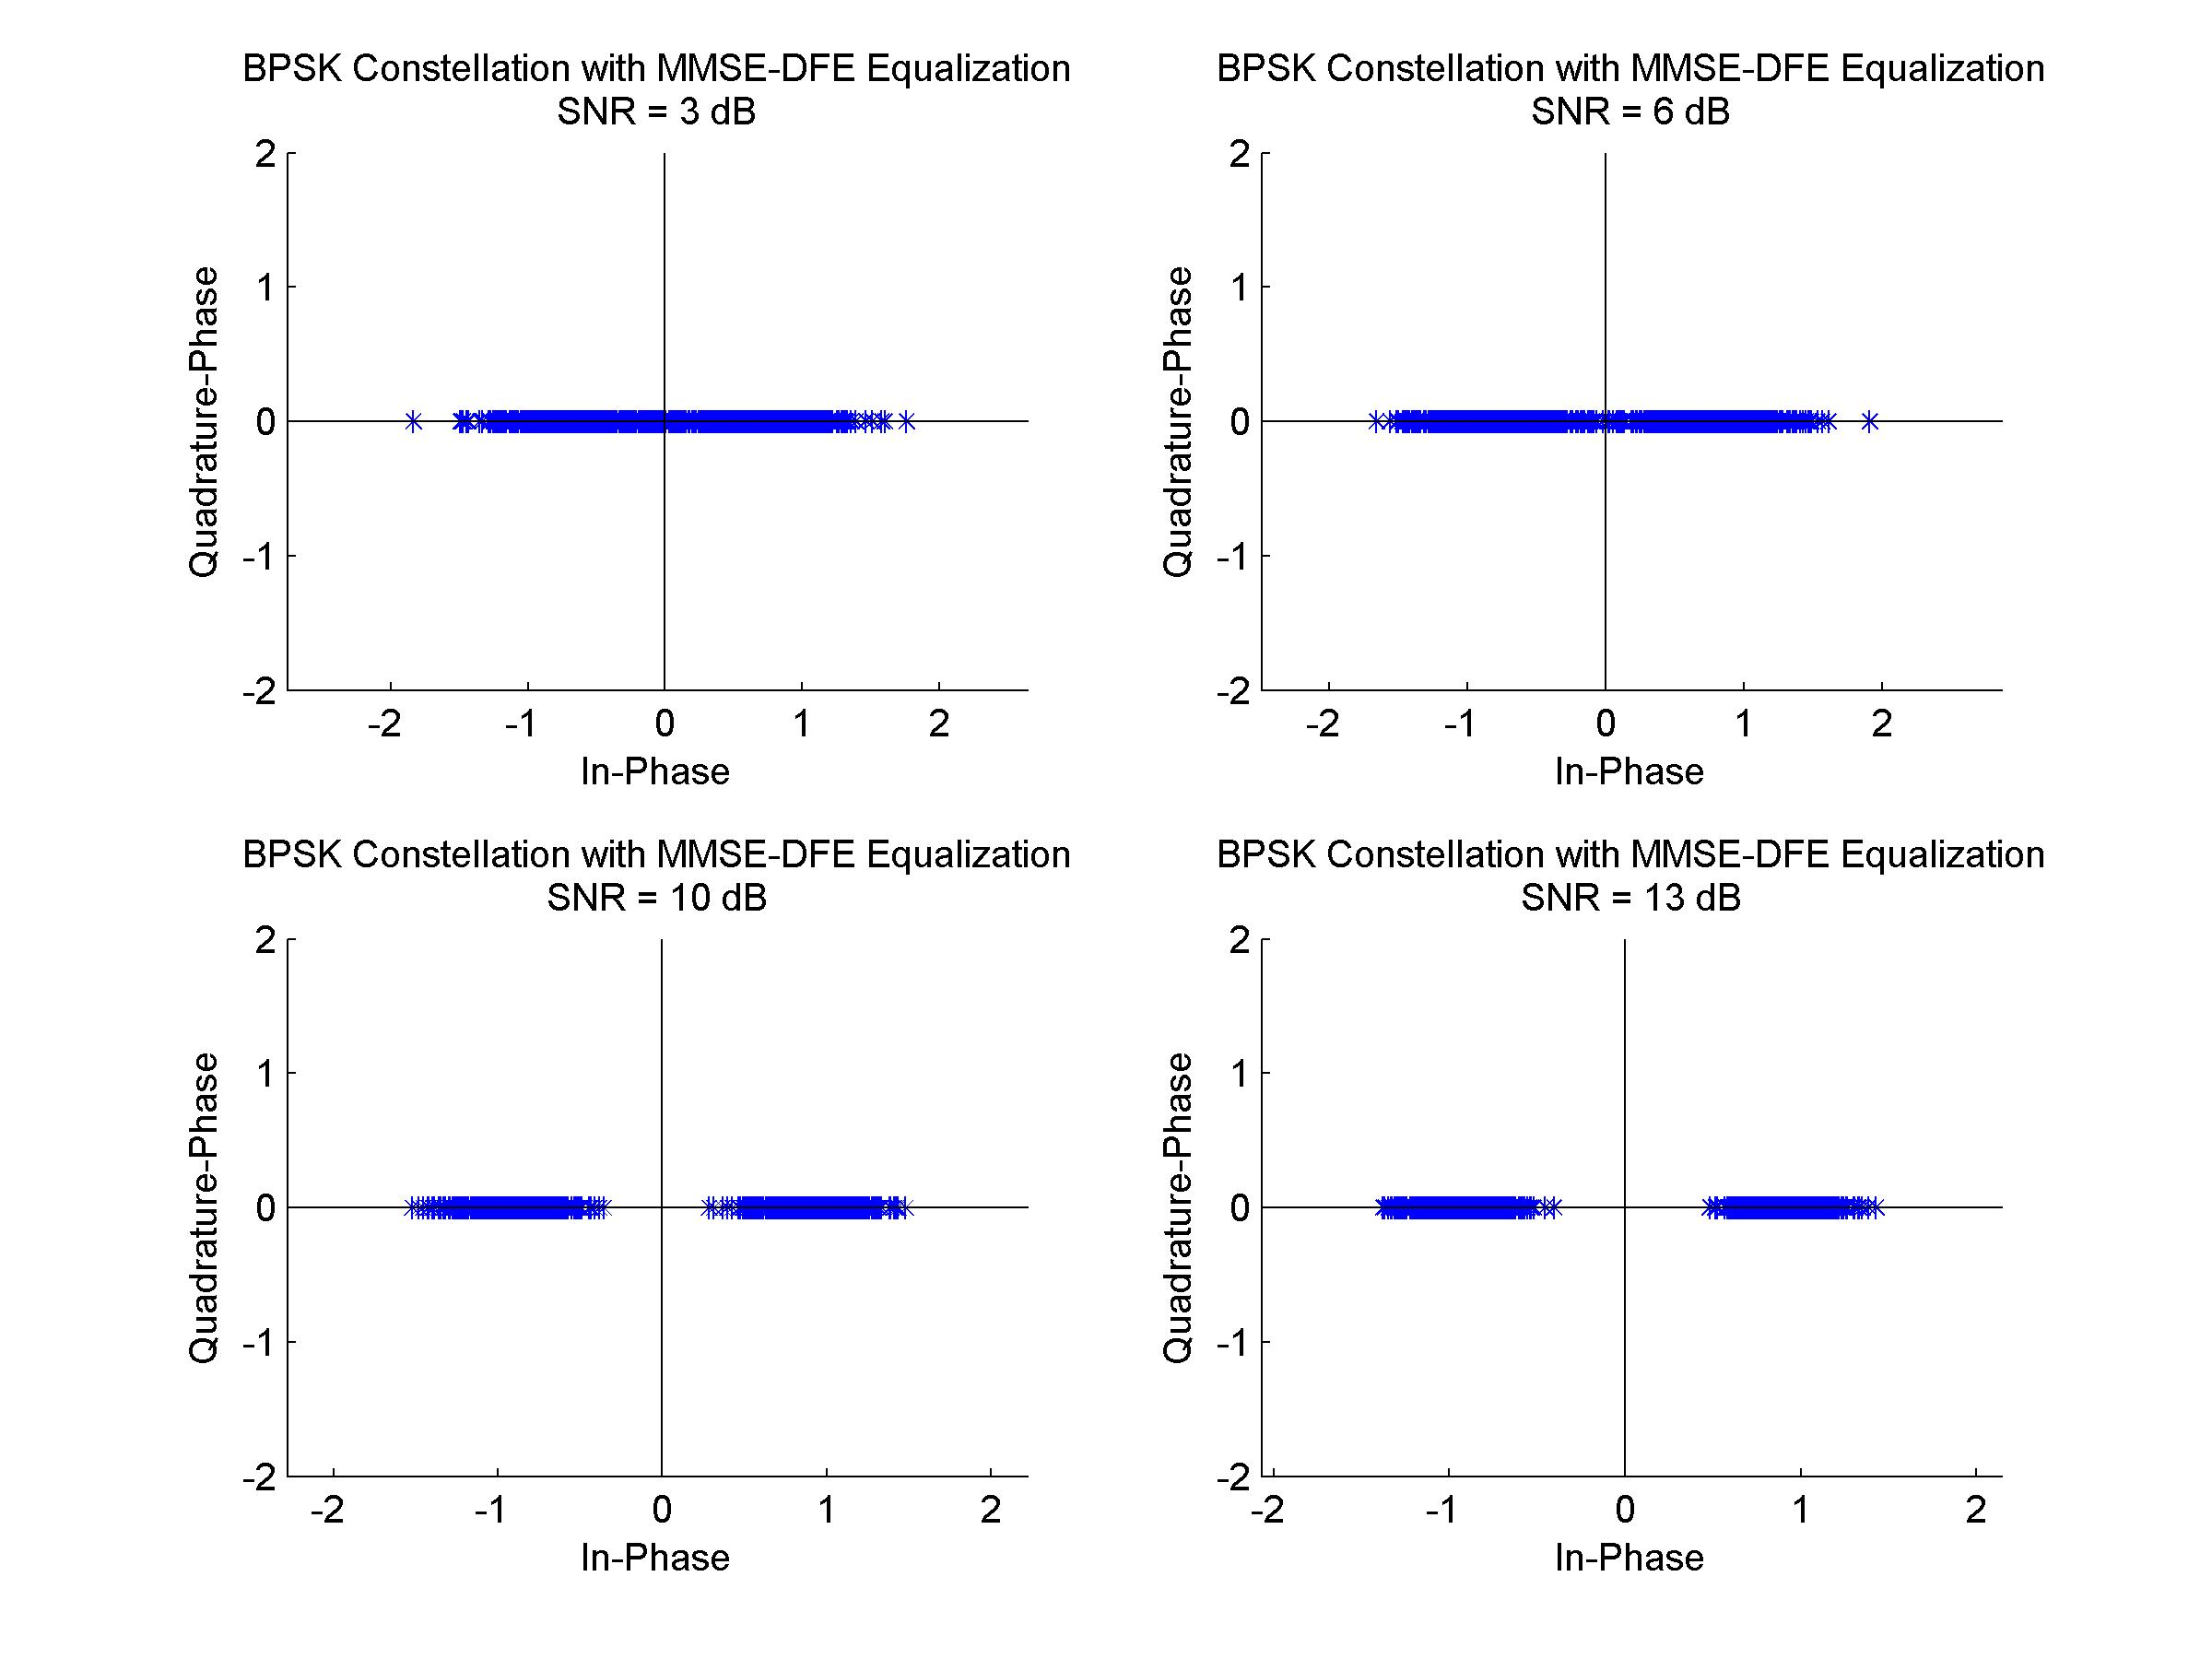
\includegraphics[width=0.7\textwidth]{bpConstMMSEDFE1.jpg}
\caption{Constellation plot for a BPSK modulated signal with MMSE-DFE equalization under channel reponse $h_1(t)$}
\end{figure}

\begin{figure}[H]
\centering
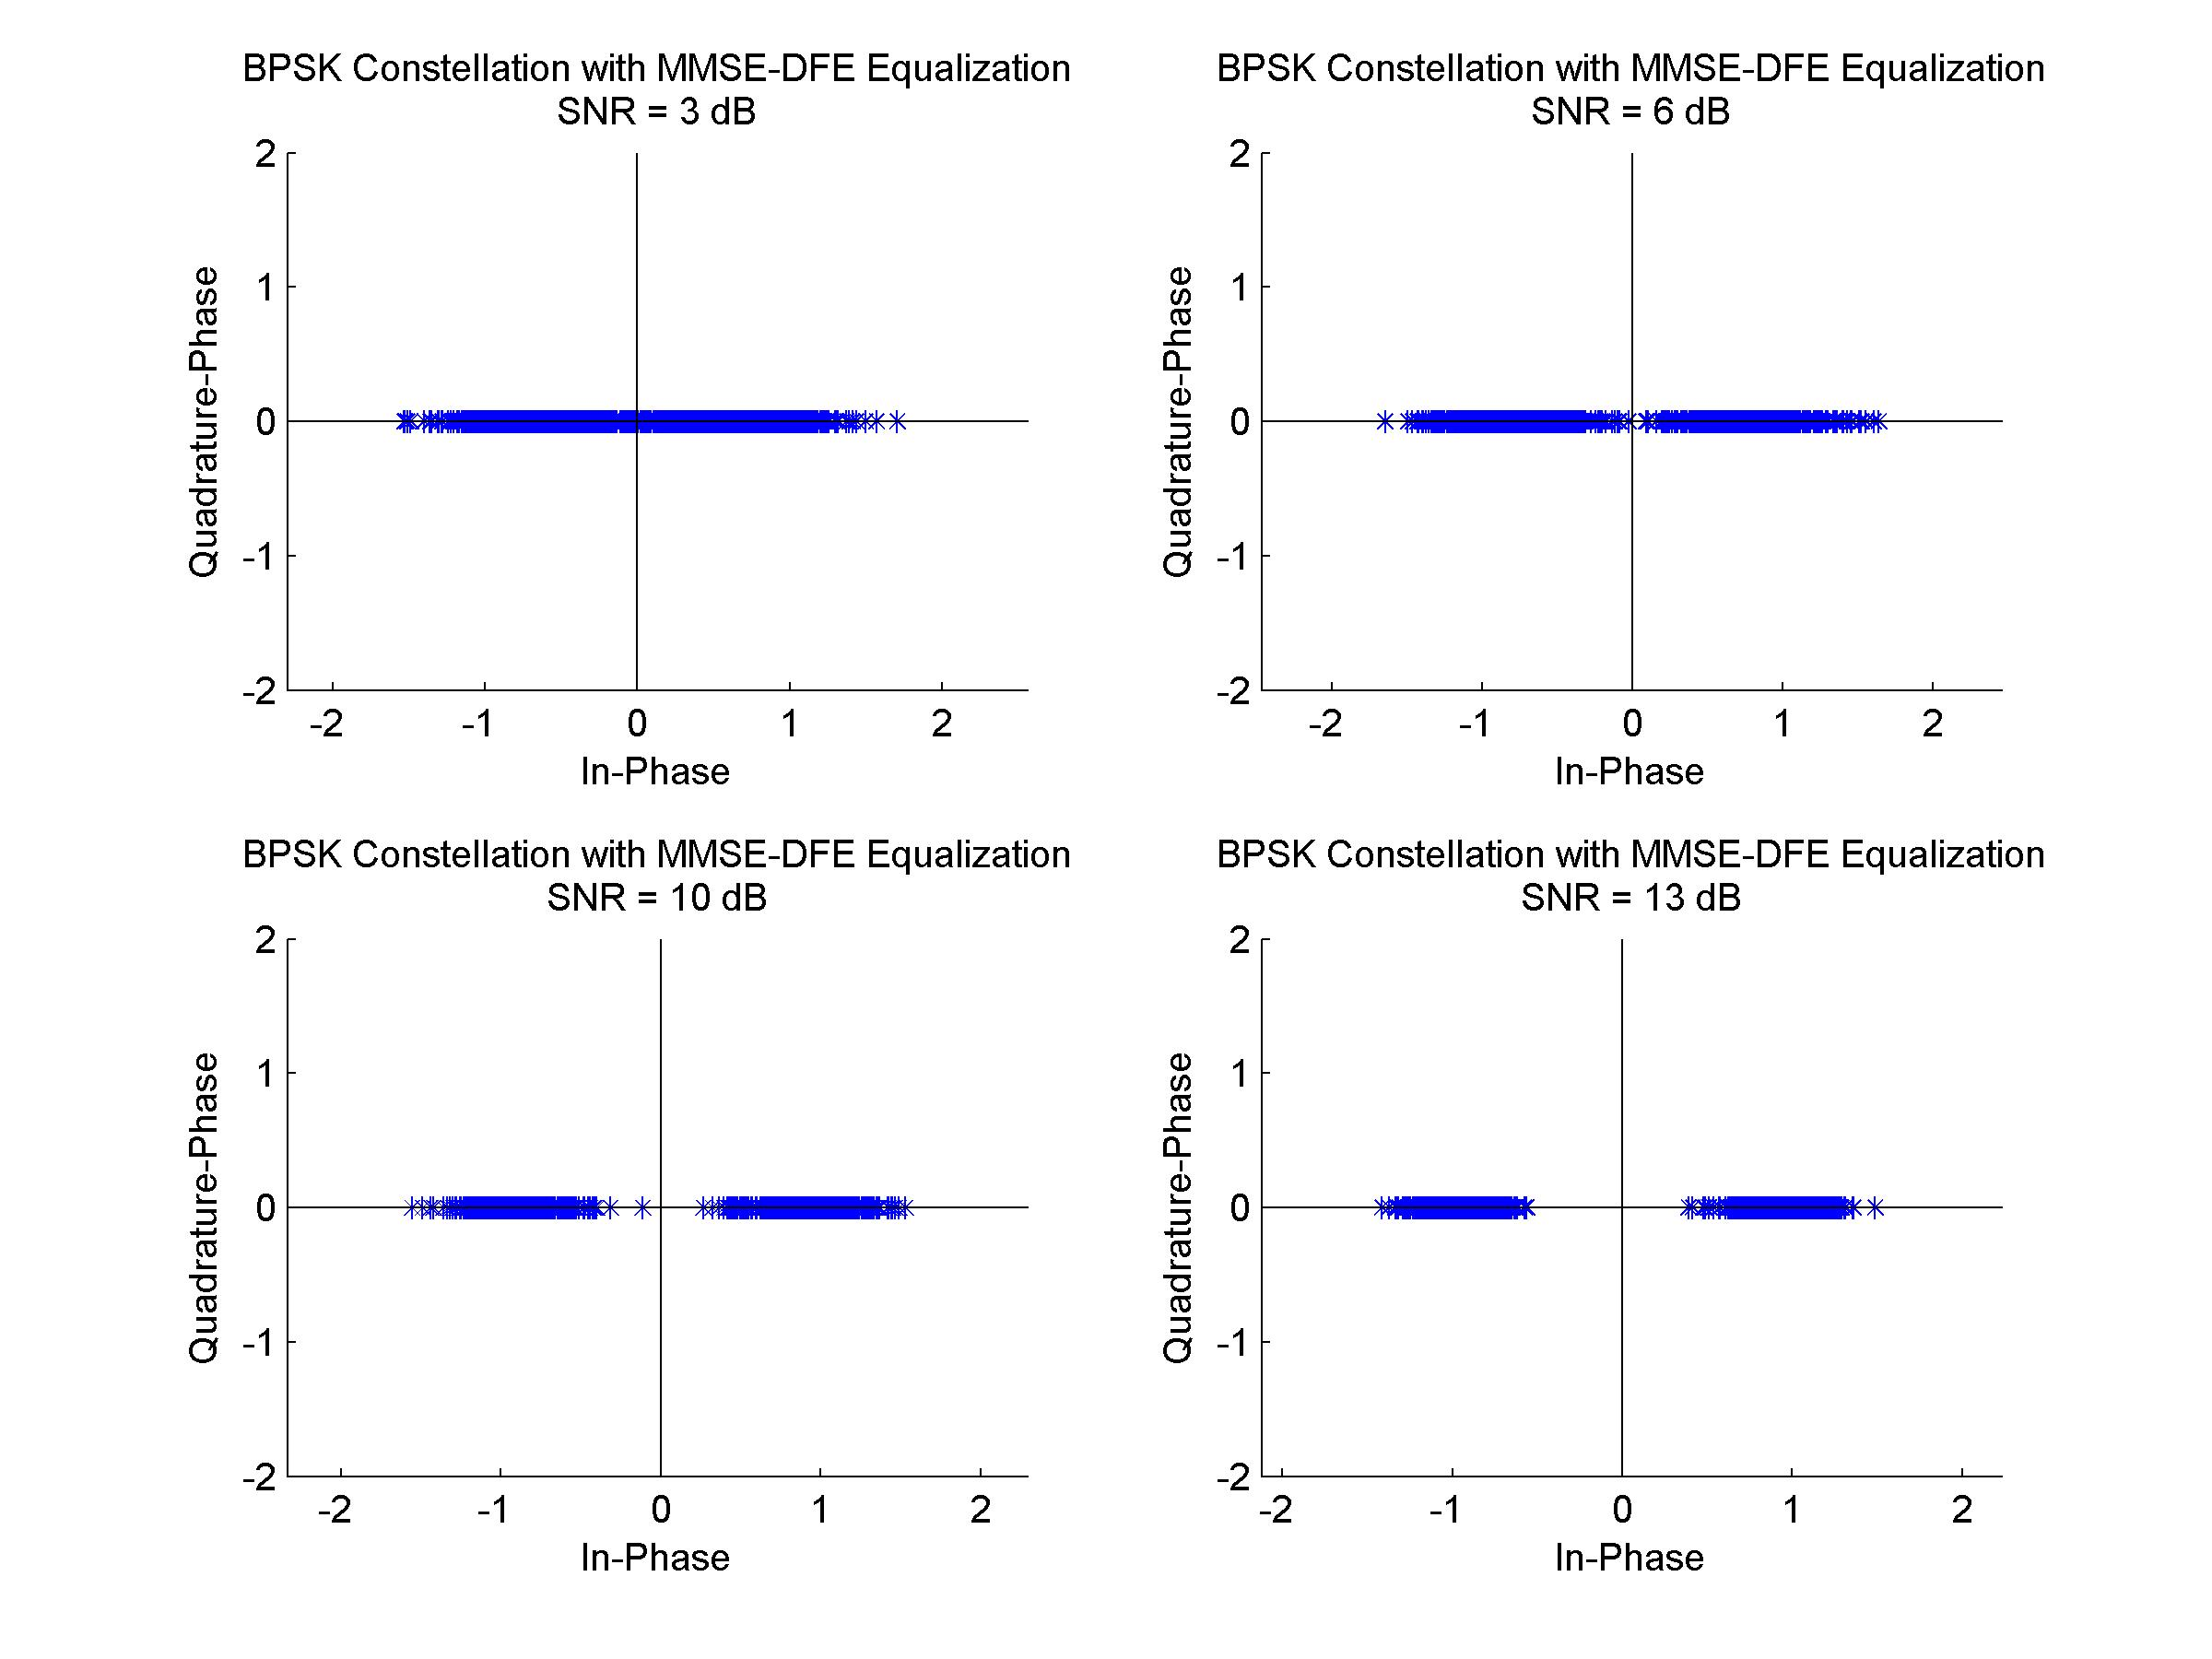
\includegraphics[width=0.7\textwidth]{bpConstMMSEDFE2.jpg}
\caption{Constellation plot for a BPSK modulated signal with MMSE-DFE equalization under channel reponse $h_2(t)$}
\end{figure}

\begin{figure}[H]
\centering
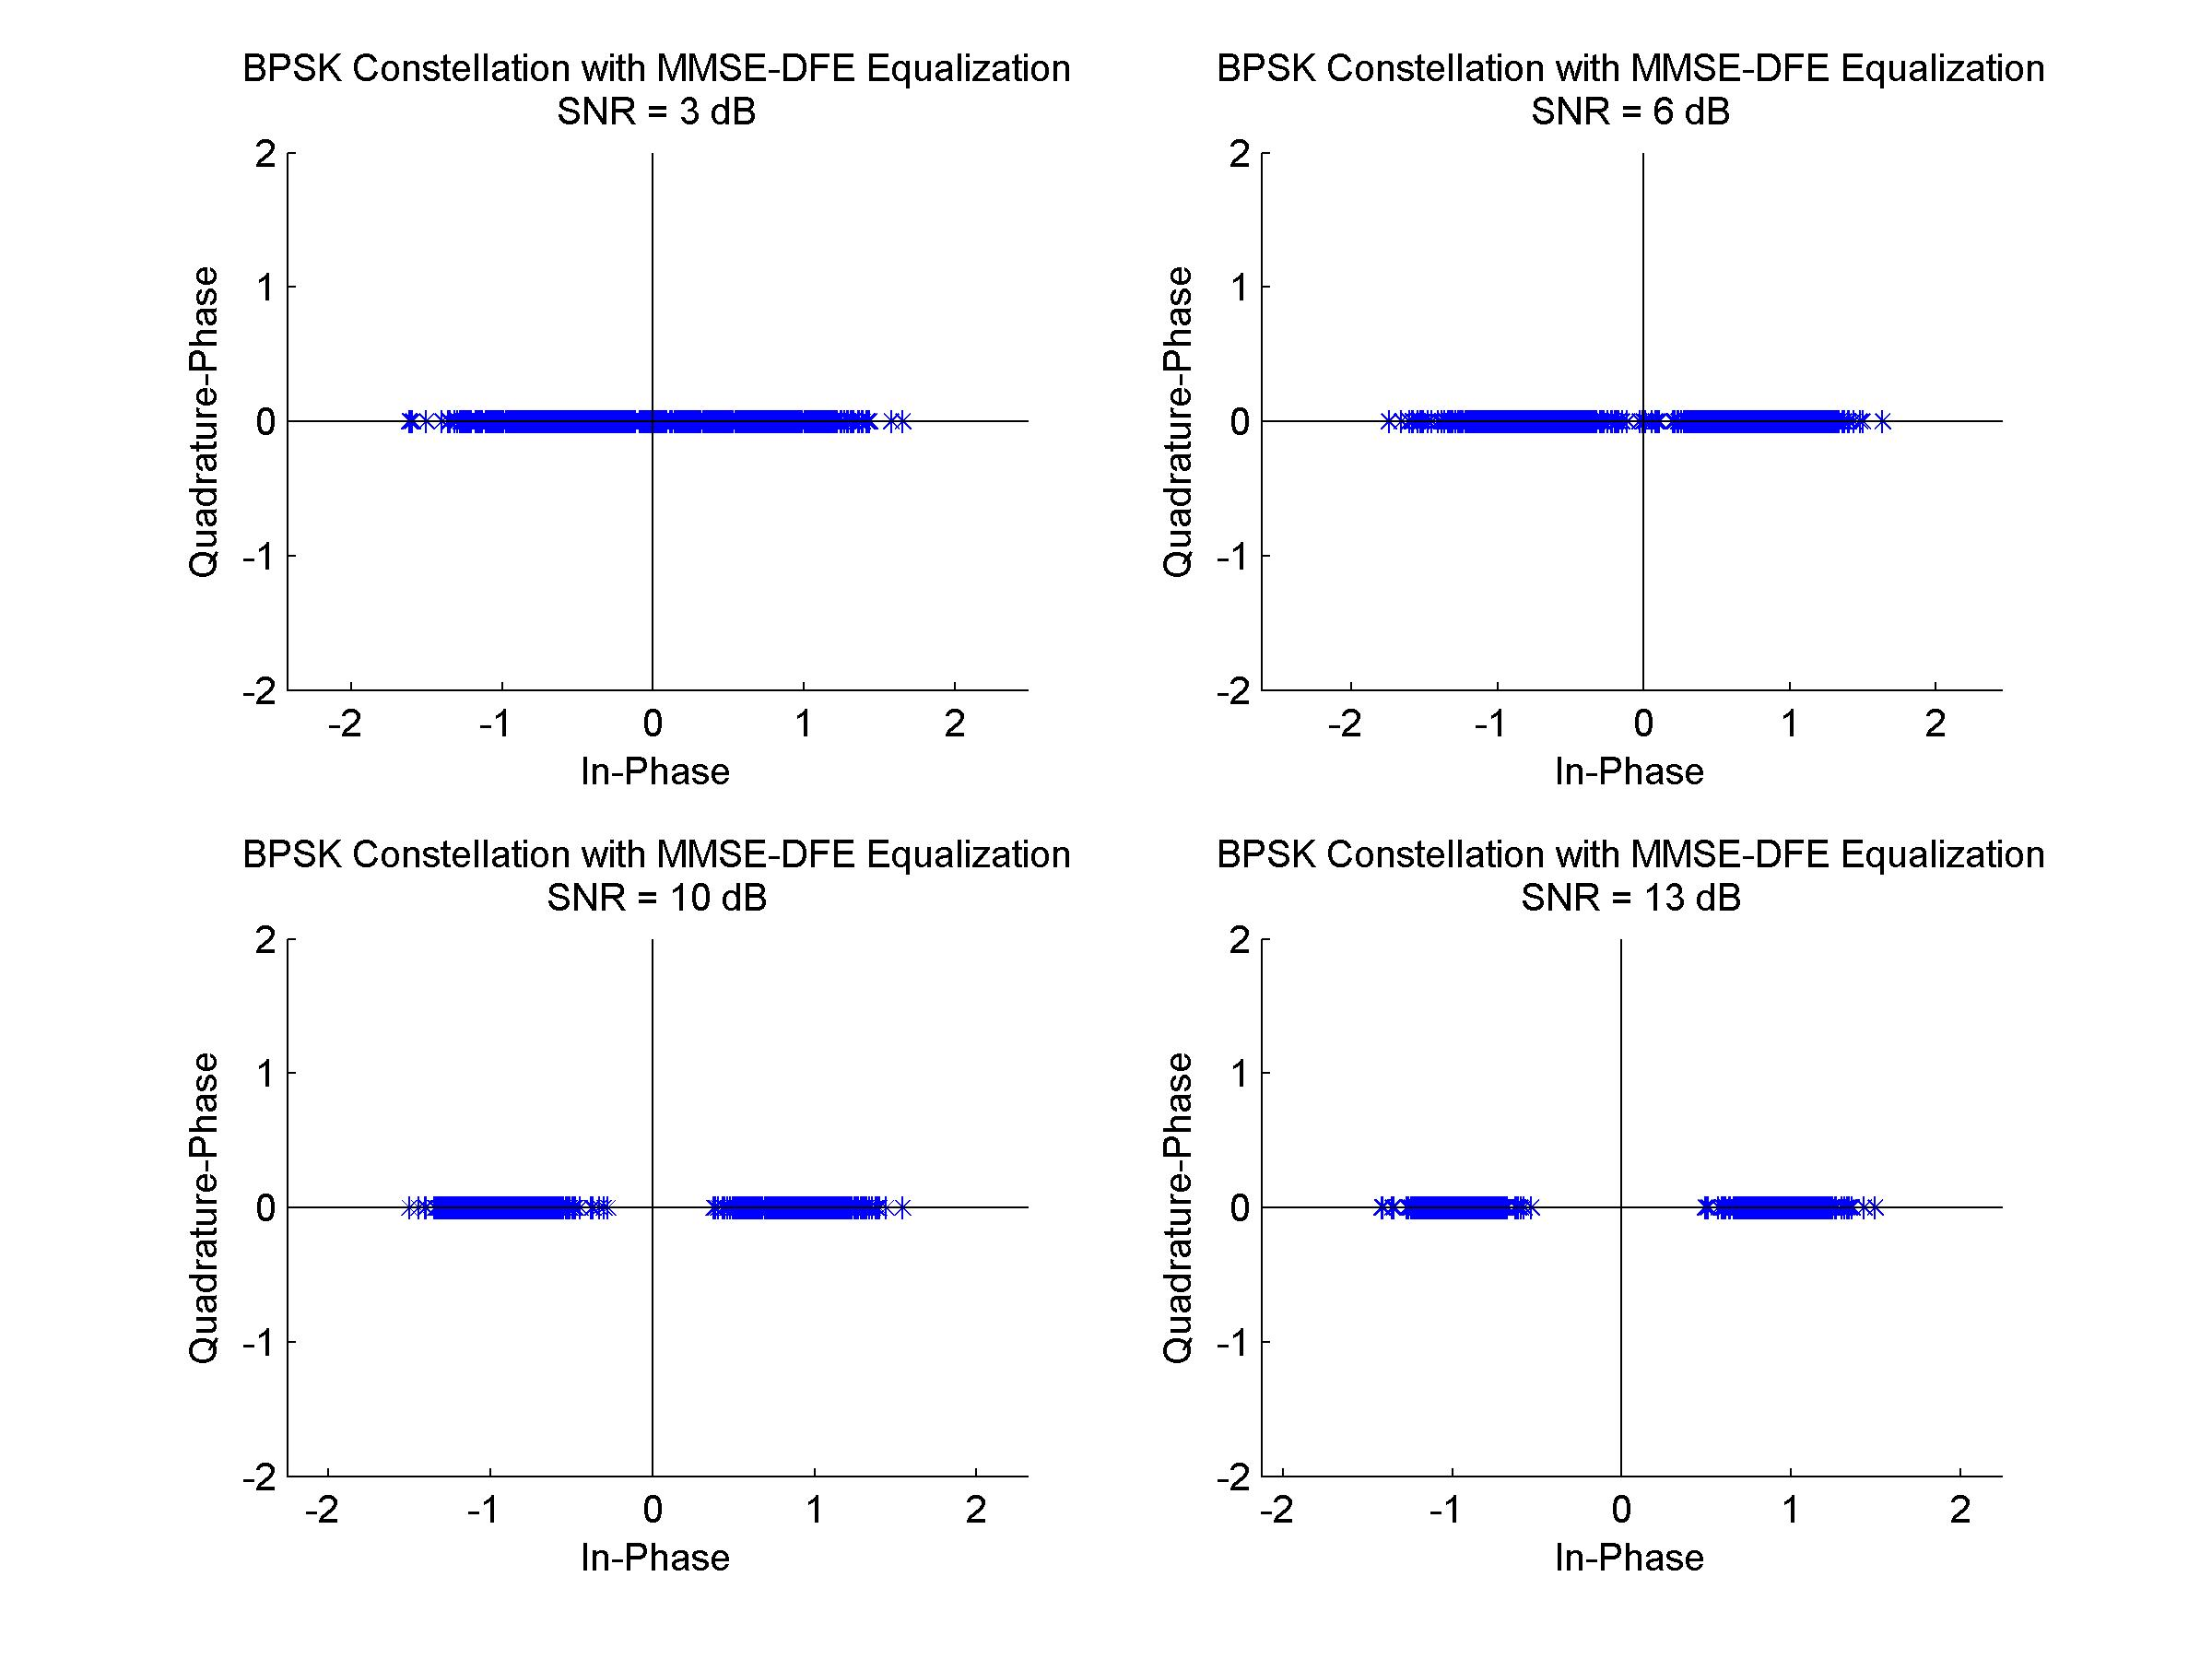
\includegraphics[width=0.7\textwidth]{bpConstMMSEDFE3.jpg}
\caption{Constellation plot for a BPSK modulated signal with MMSE-DFE equalization under channel reponse $h_3(t)$}
\end{figure}


\subsubsection{QPSK with No Equalization}

\begin{figure}[H]
\centering
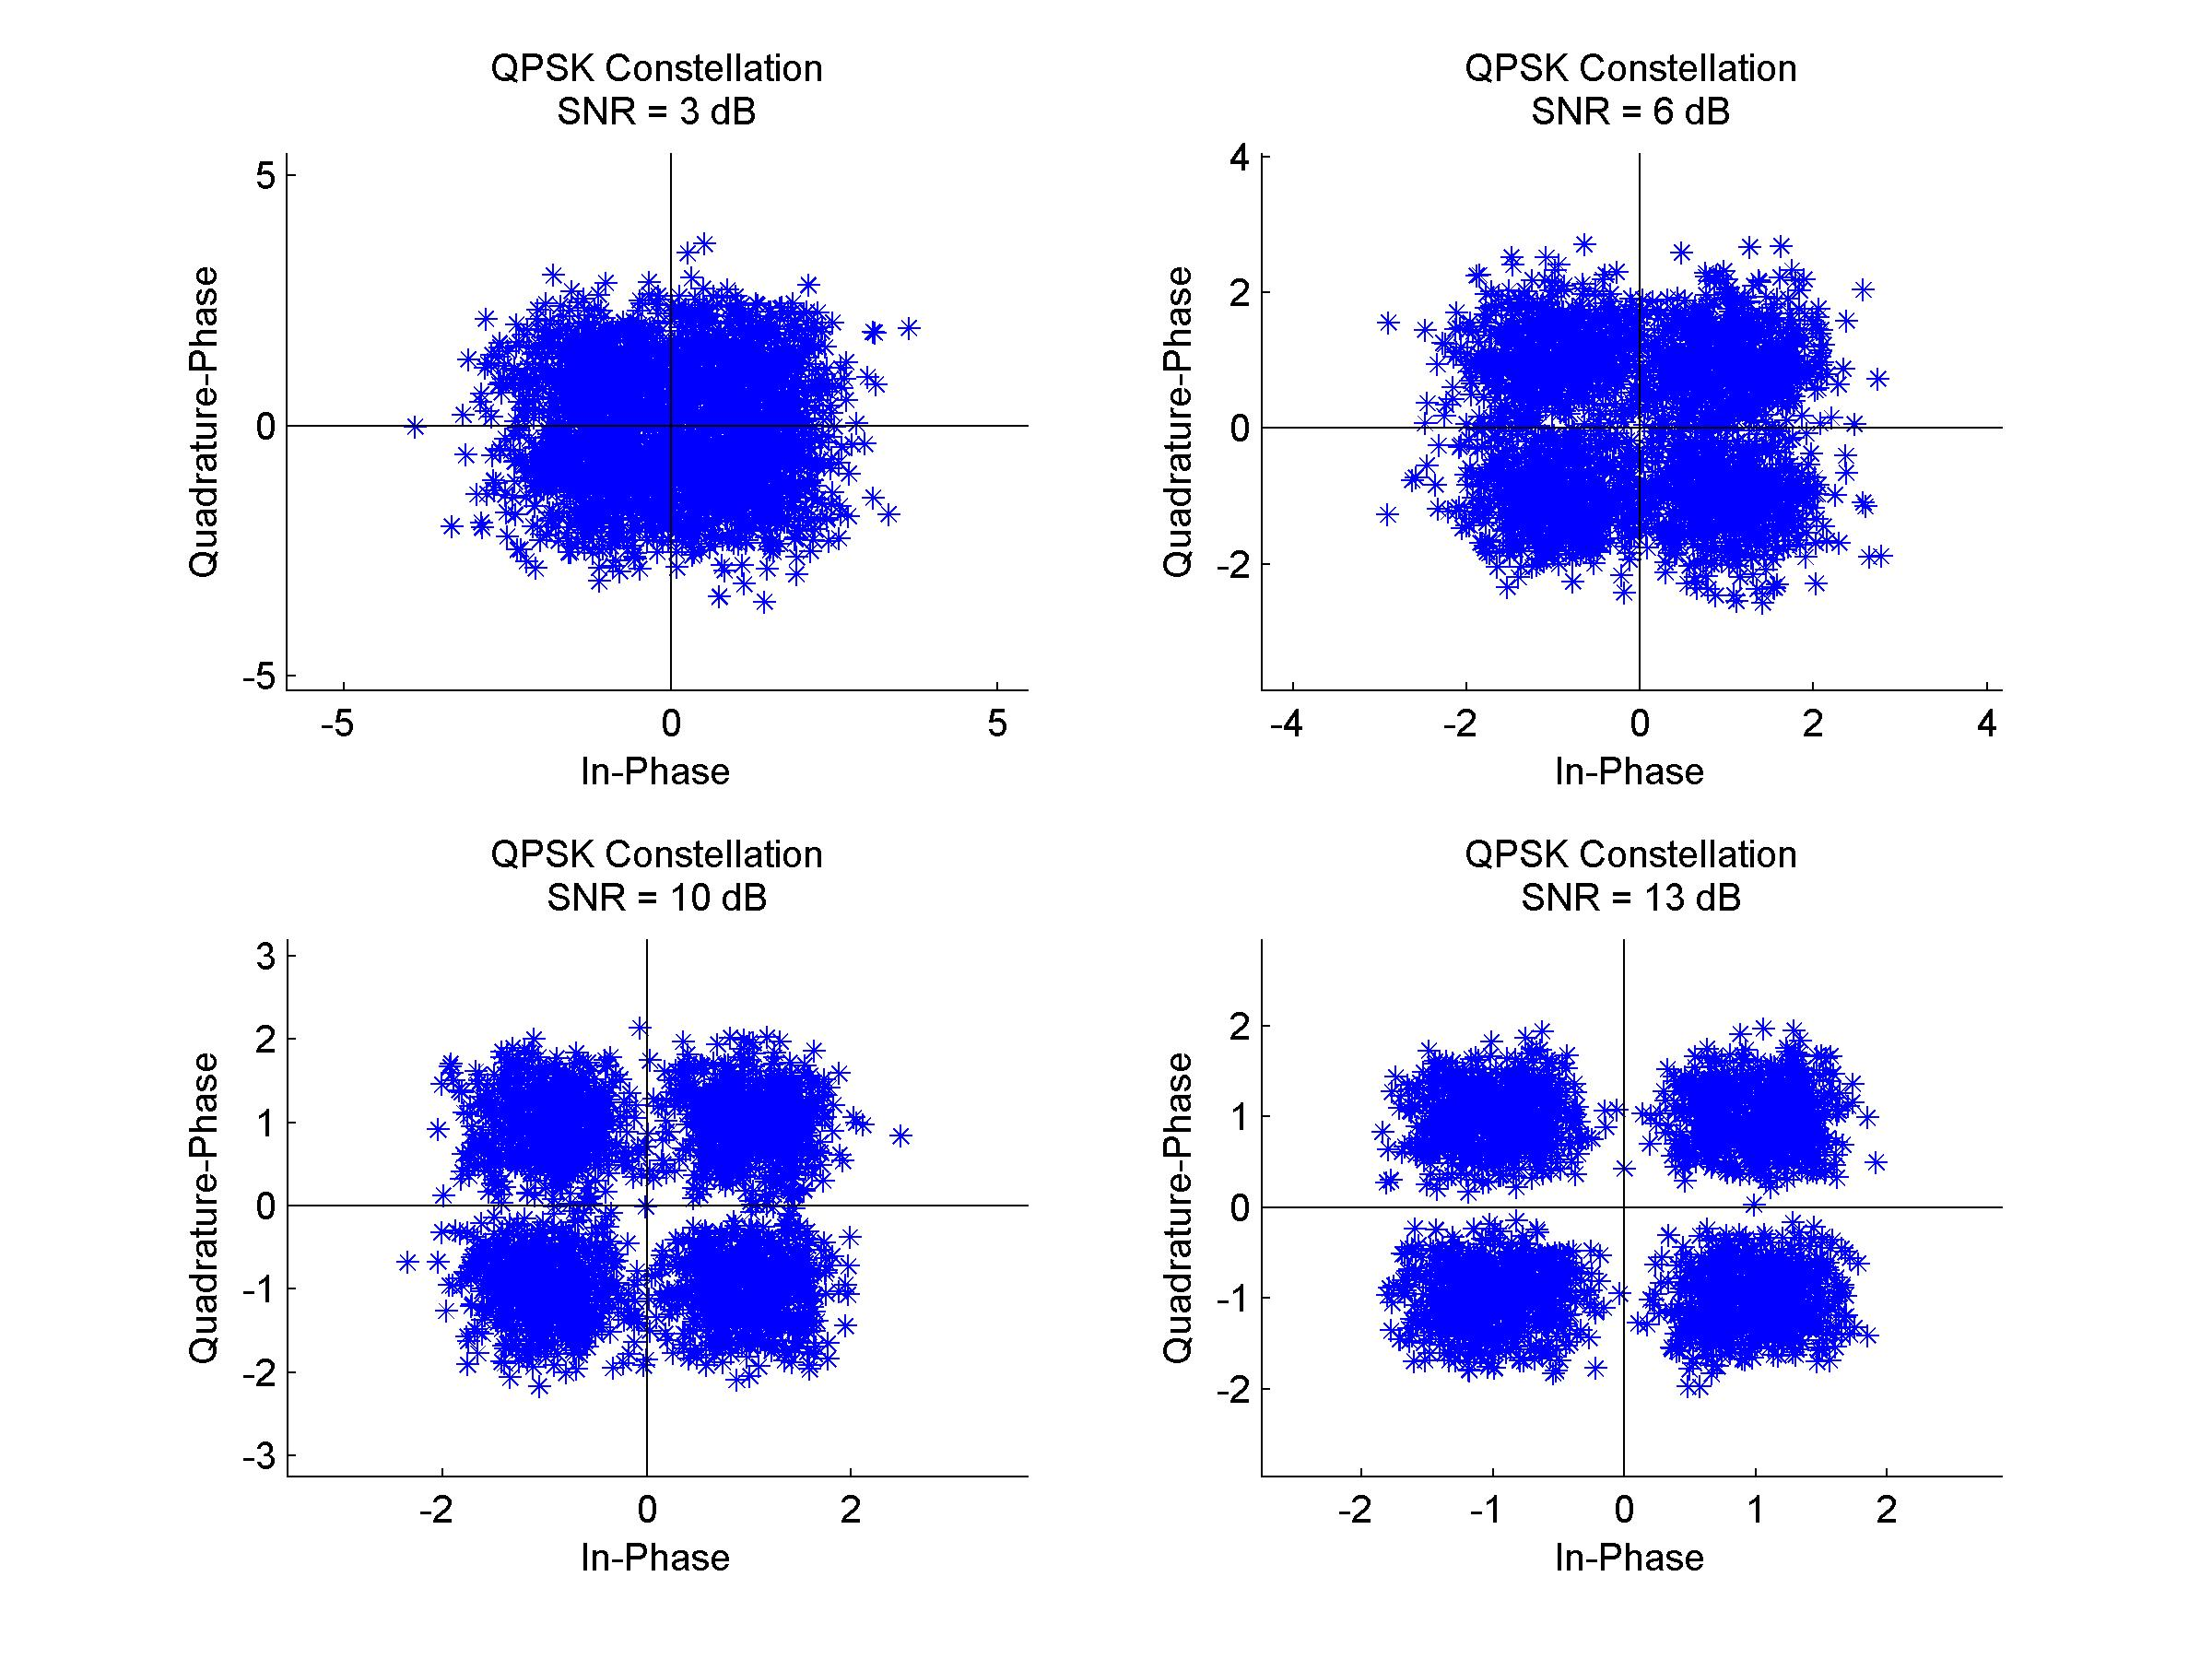
\includegraphics[width=0.7\textwidth]{qpConst1.jpg}
\caption{Constellation plot for a QPSK modulated signal with no equalization under channel reponse $h_1(t)$}
\end{figure}

\begin{figure}[H]
\centering
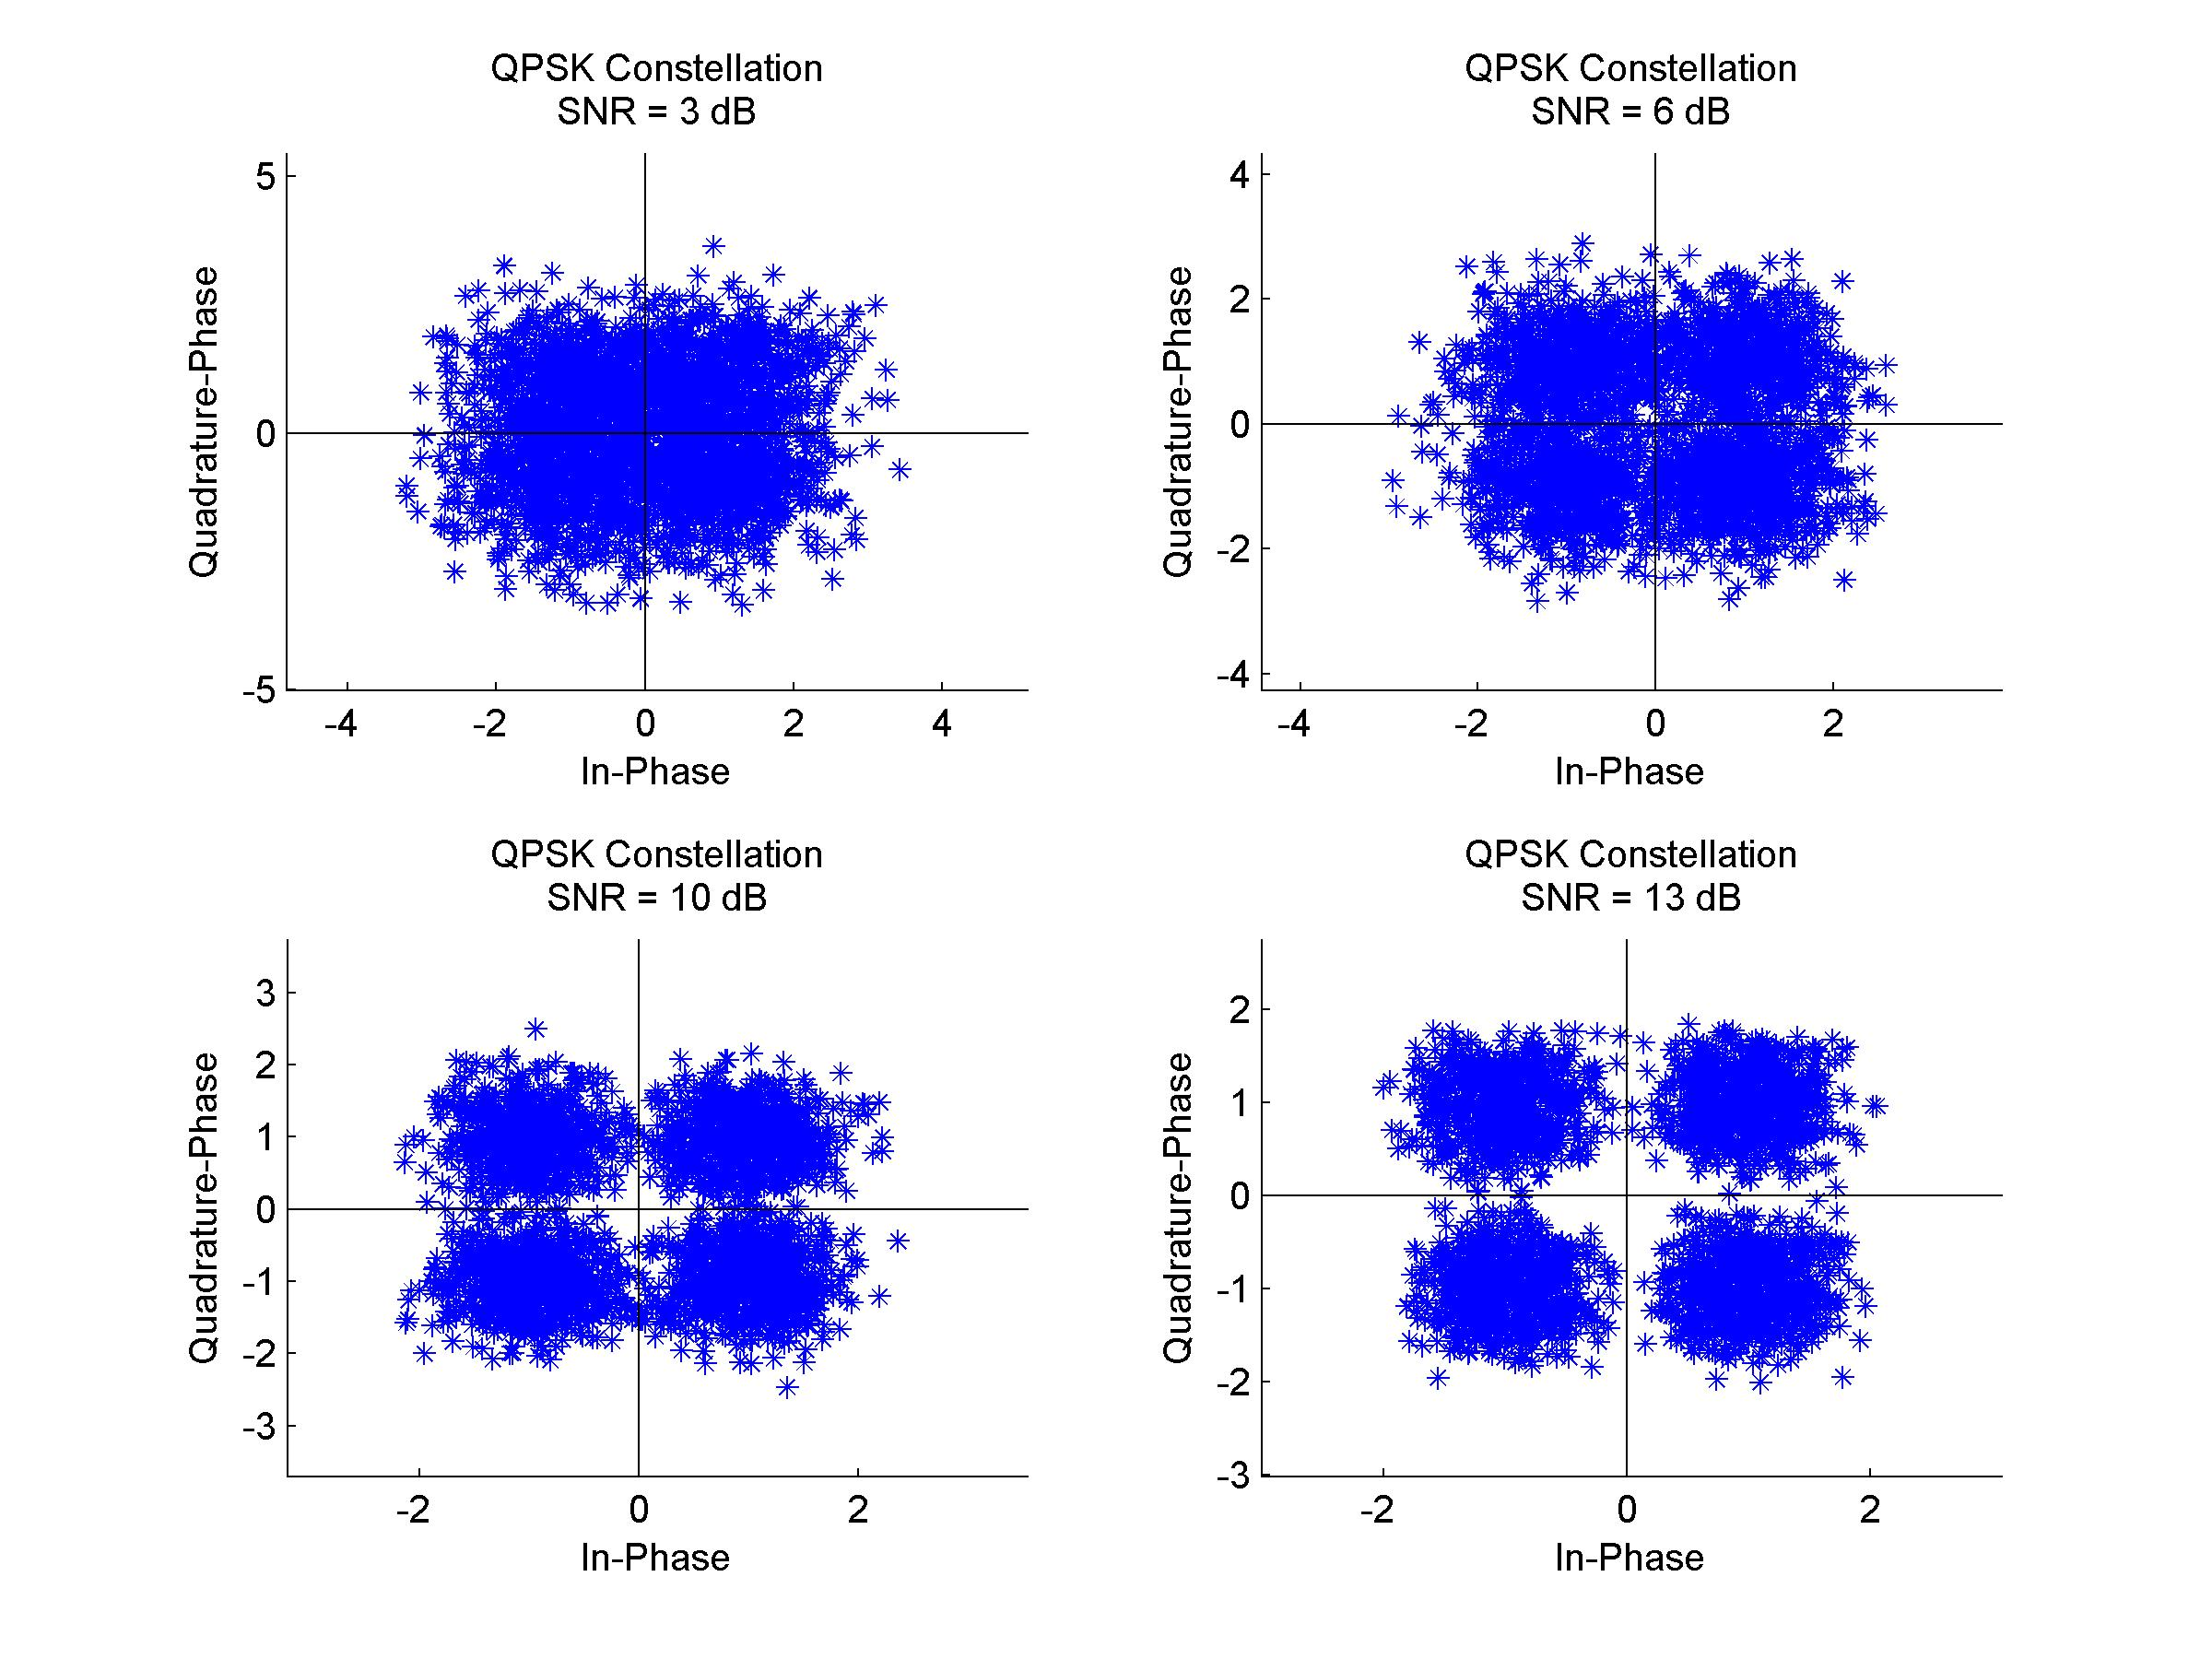
\includegraphics[width=0.7\textwidth]{qpConst2.jpg}
\caption{Constellation plot for a QPSK modulated signal with no equalization under channel reponse $h_2(t)$}
\end{figure}

\begin{figure}[H]
\centering
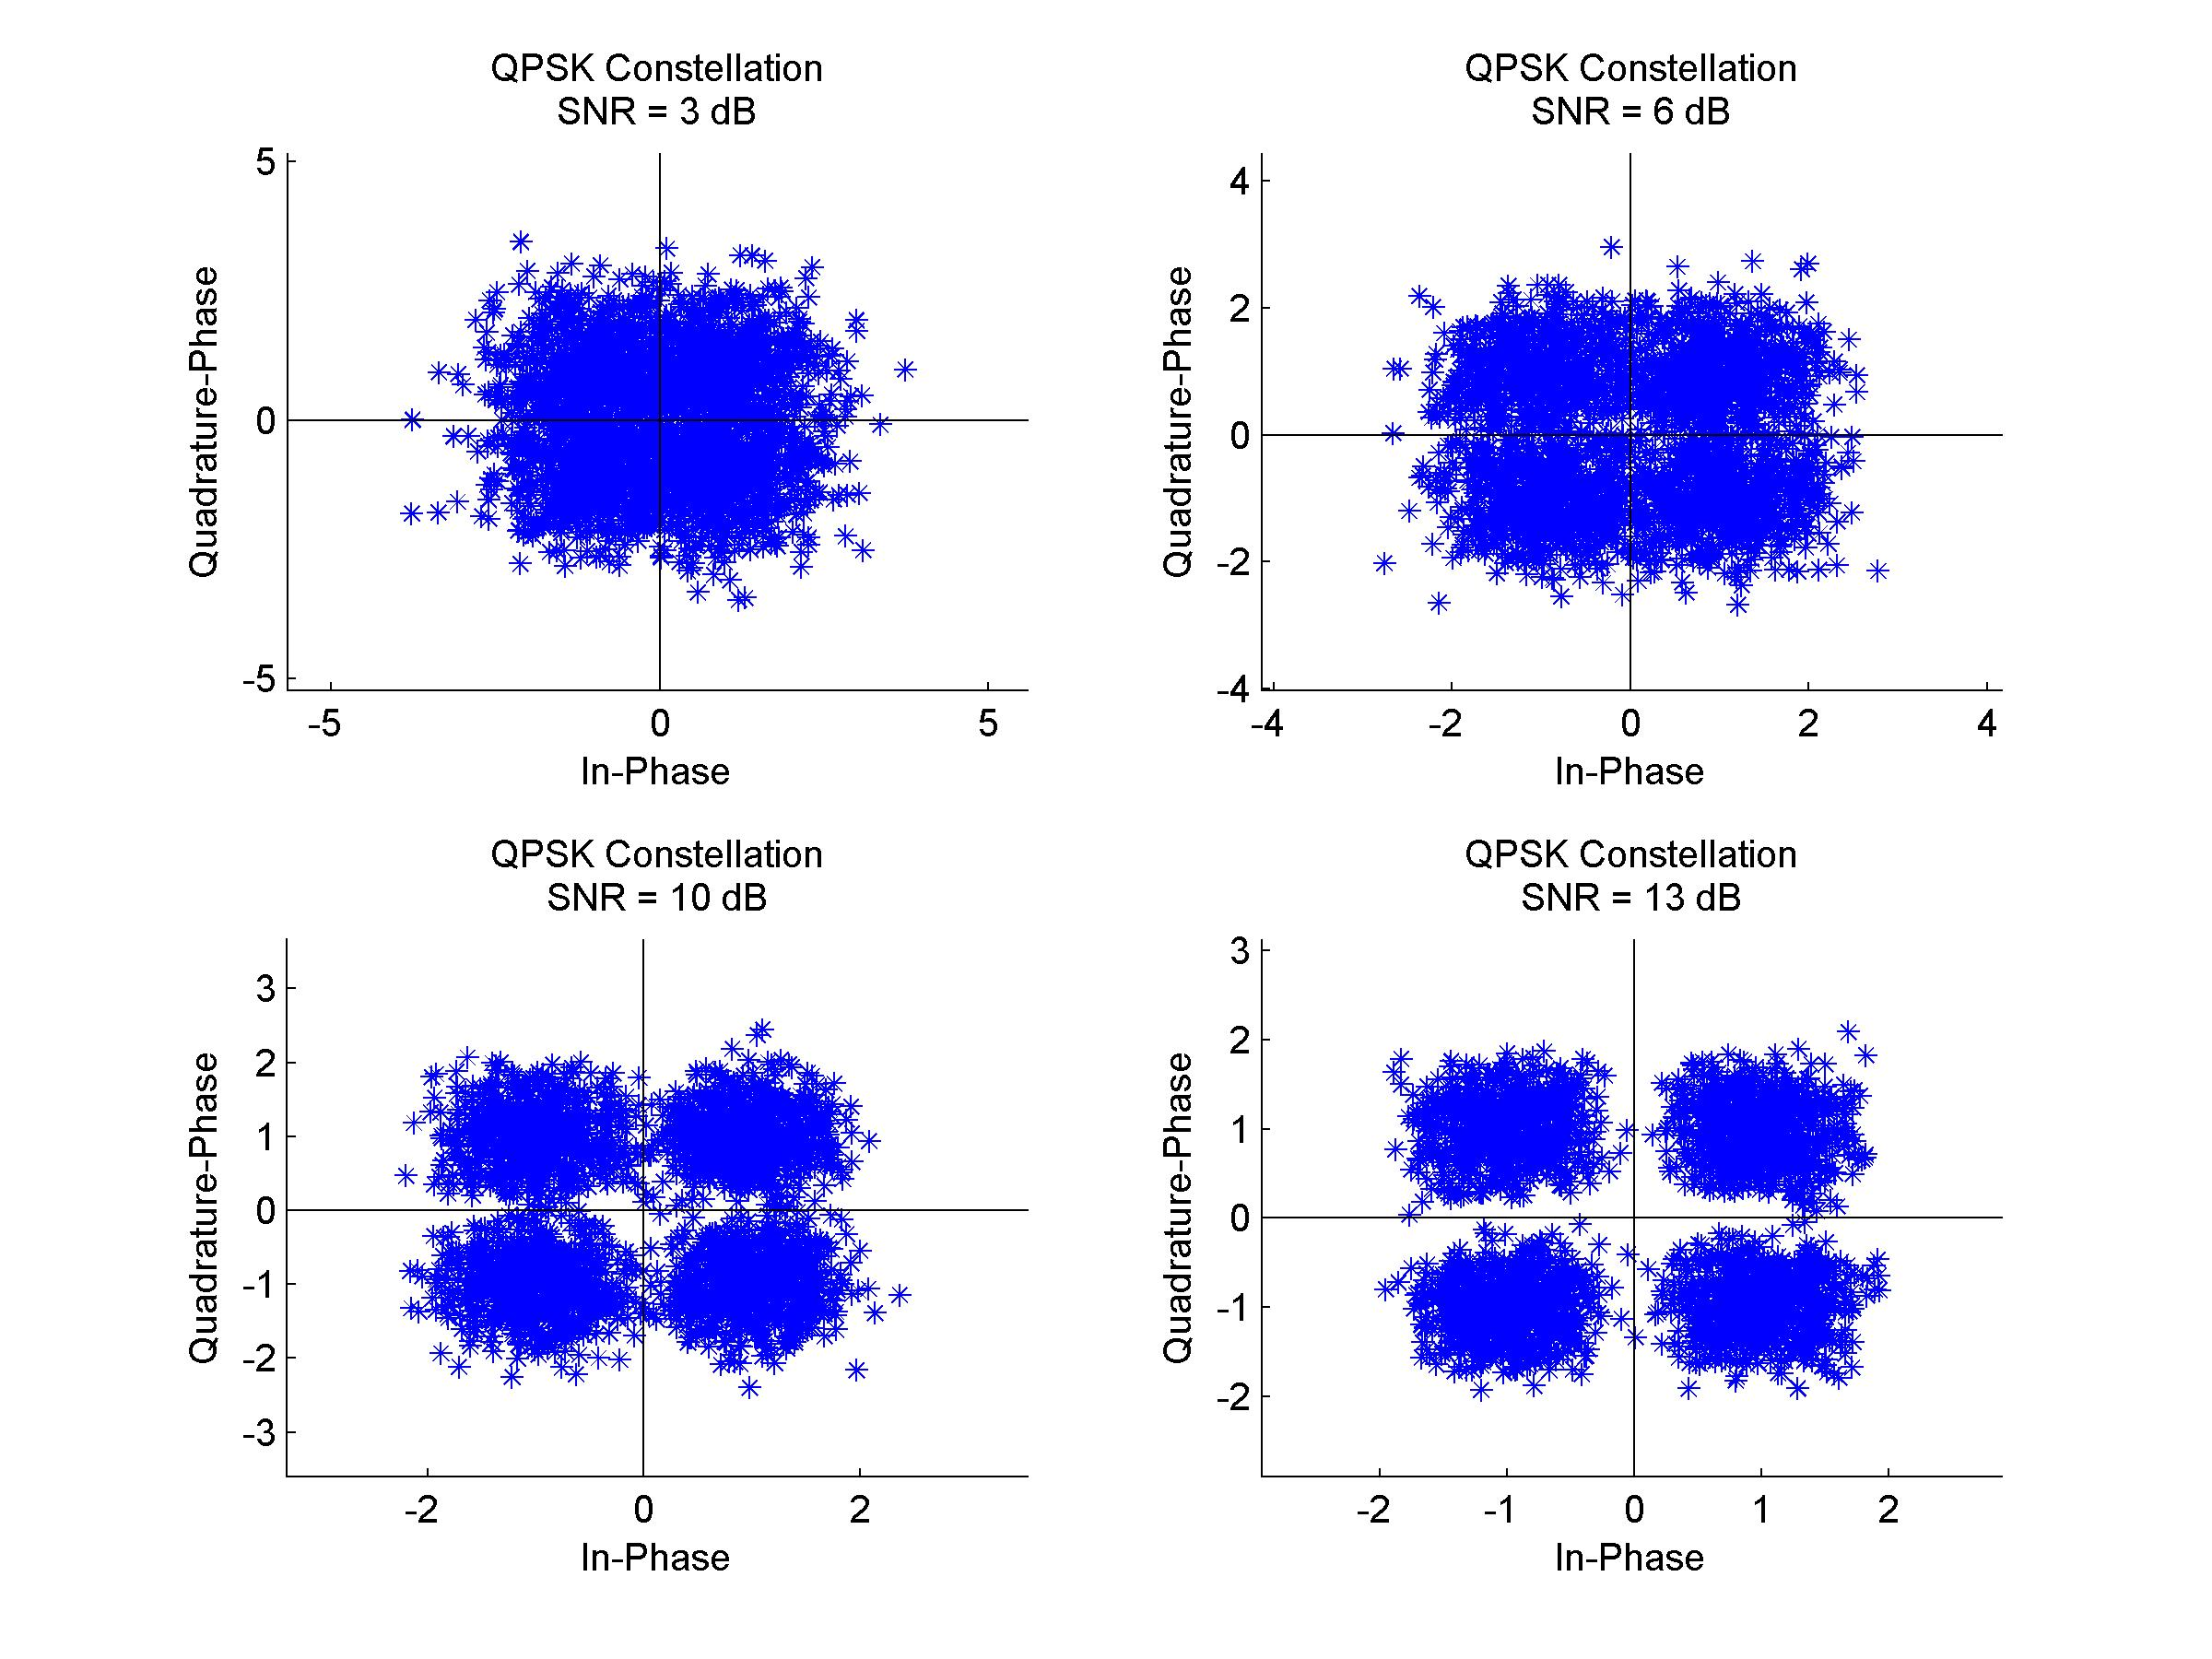
\includegraphics[width=0.7\textwidth]{qpConst3.jpg}
\caption{Constellation plot for a QPSK modulated signal with no equalization under channel reponse $h_3(t)$}
\end{figure}

\subsubsection{QPSK with ZF Equalization}

\begin{figure}[H]
\centering
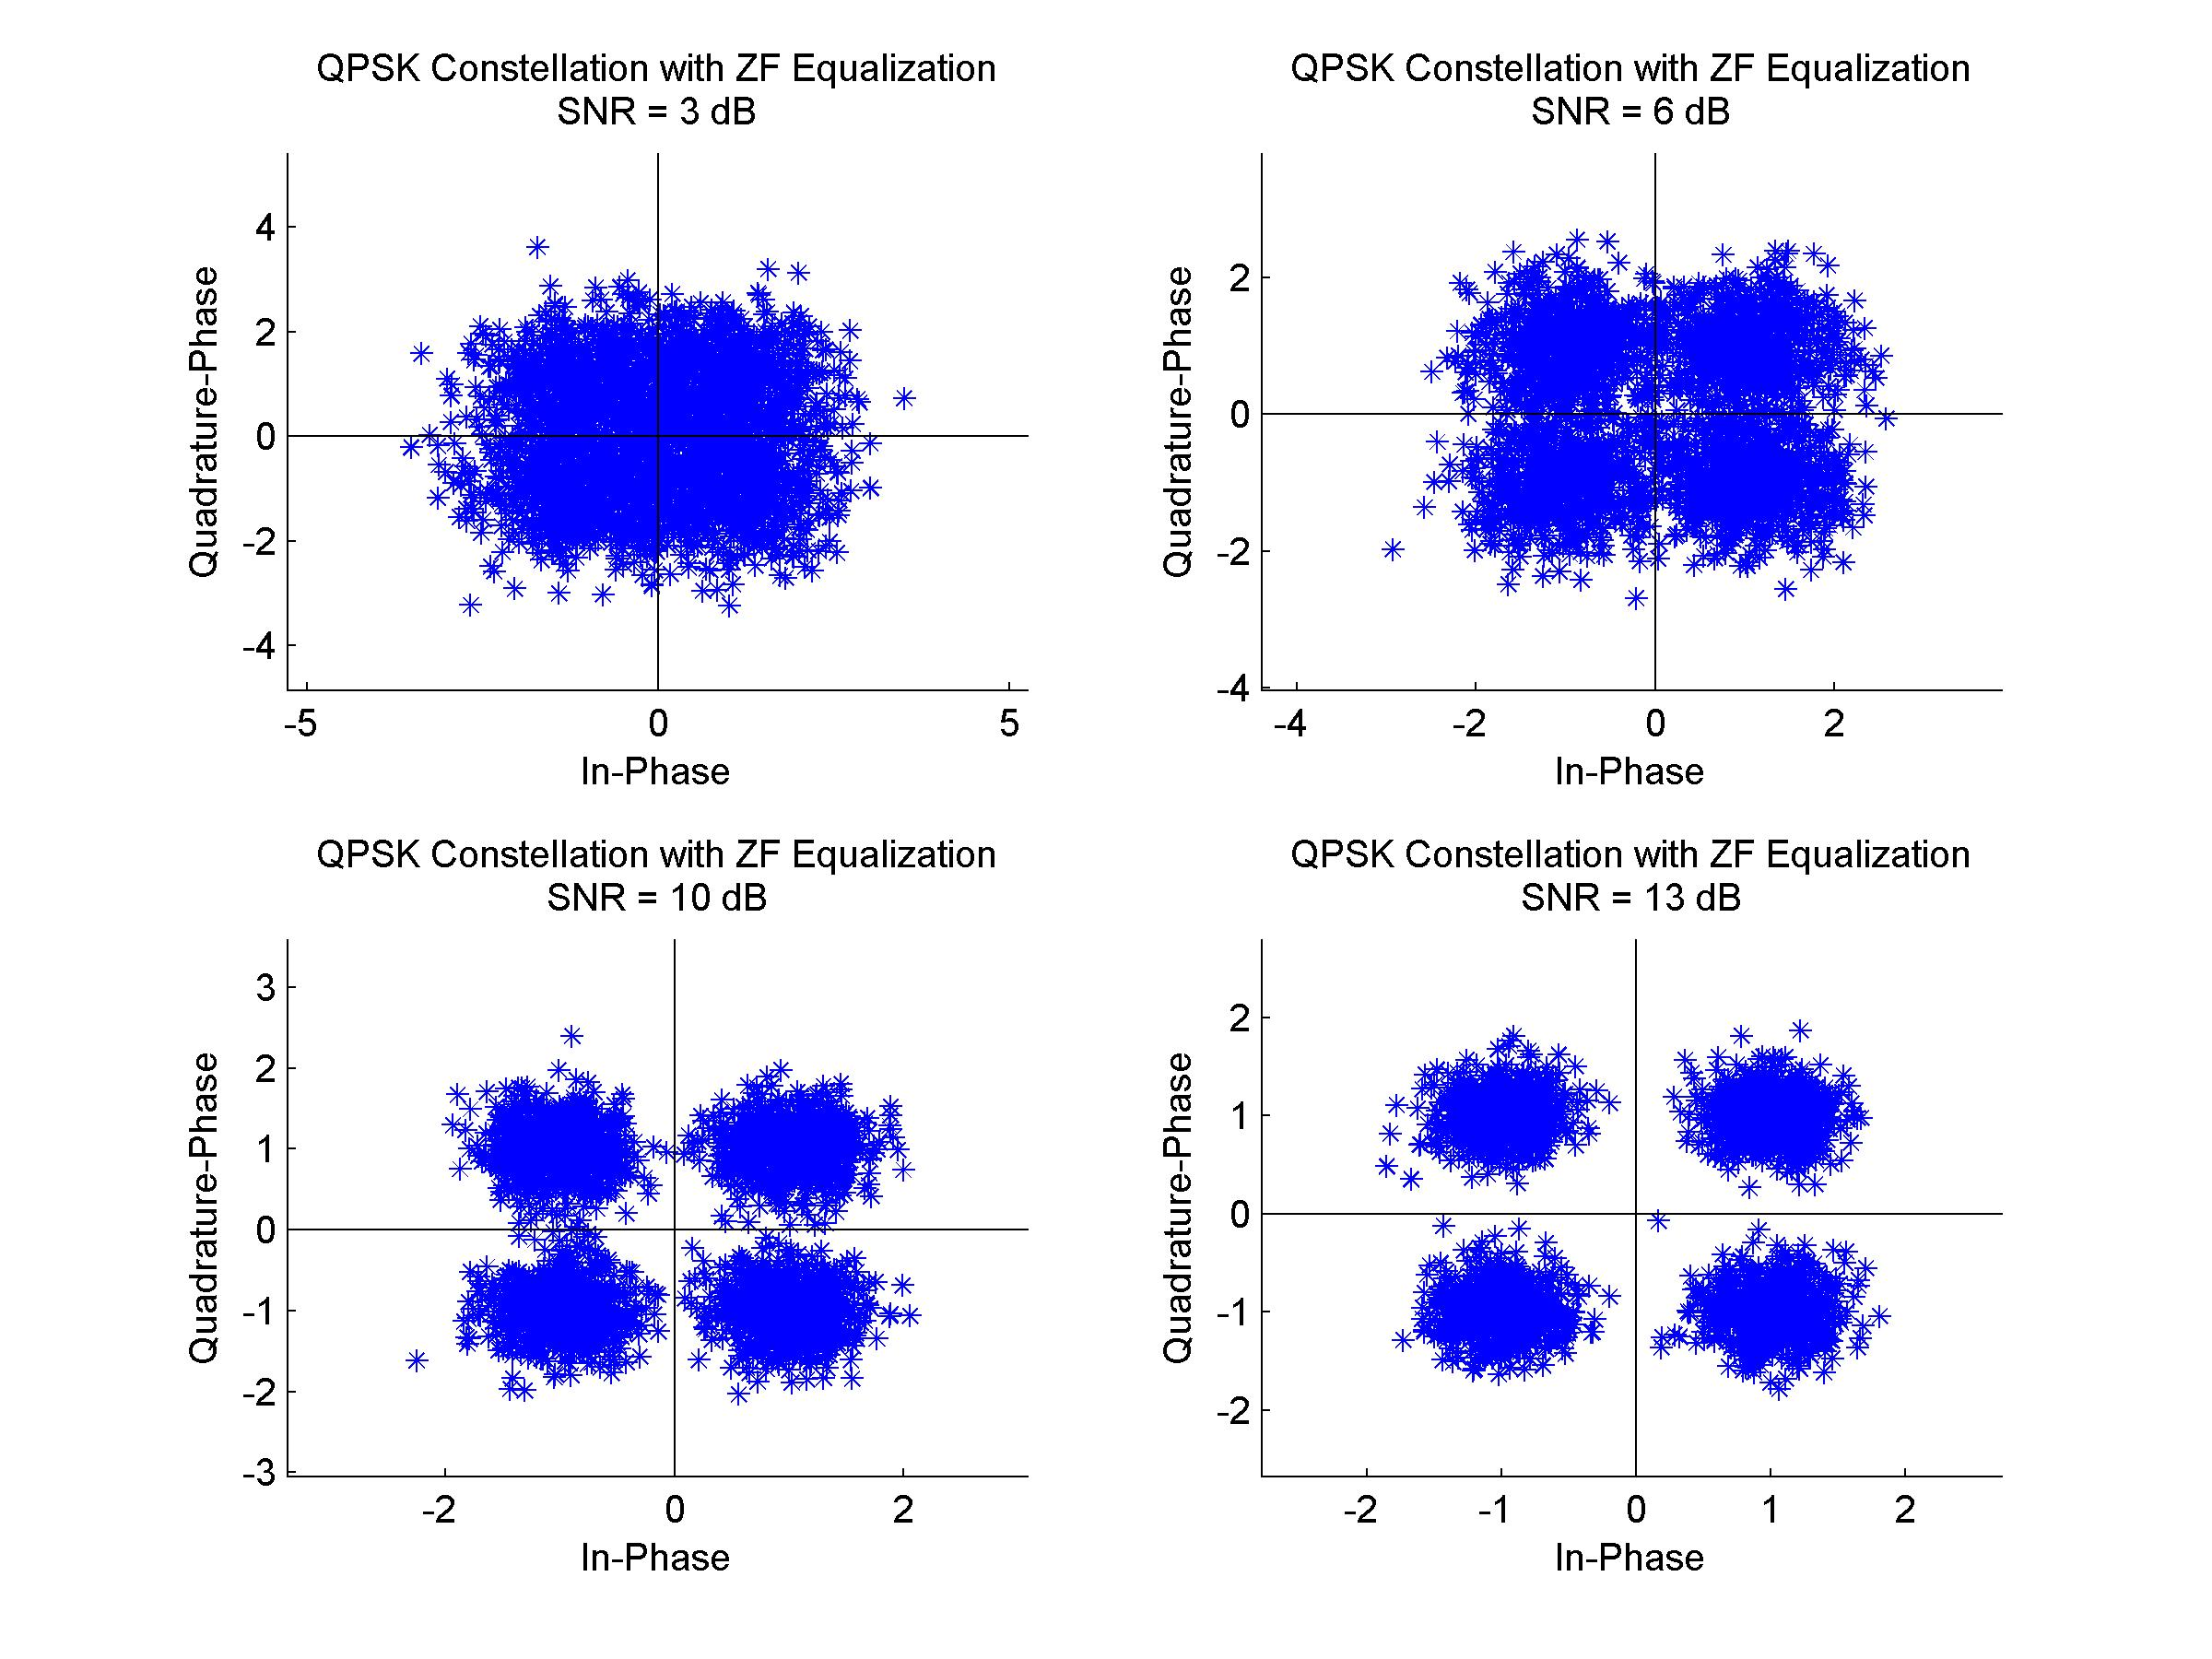
\includegraphics[width=0.7\textwidth]{qpConstZF1.jpg}
\caption{Constellation plot for a QPSK modulated signal with ZF equalization under channel reponse $h_1(t)$}
\end{figure}

\begin{figure}[H]
\centering
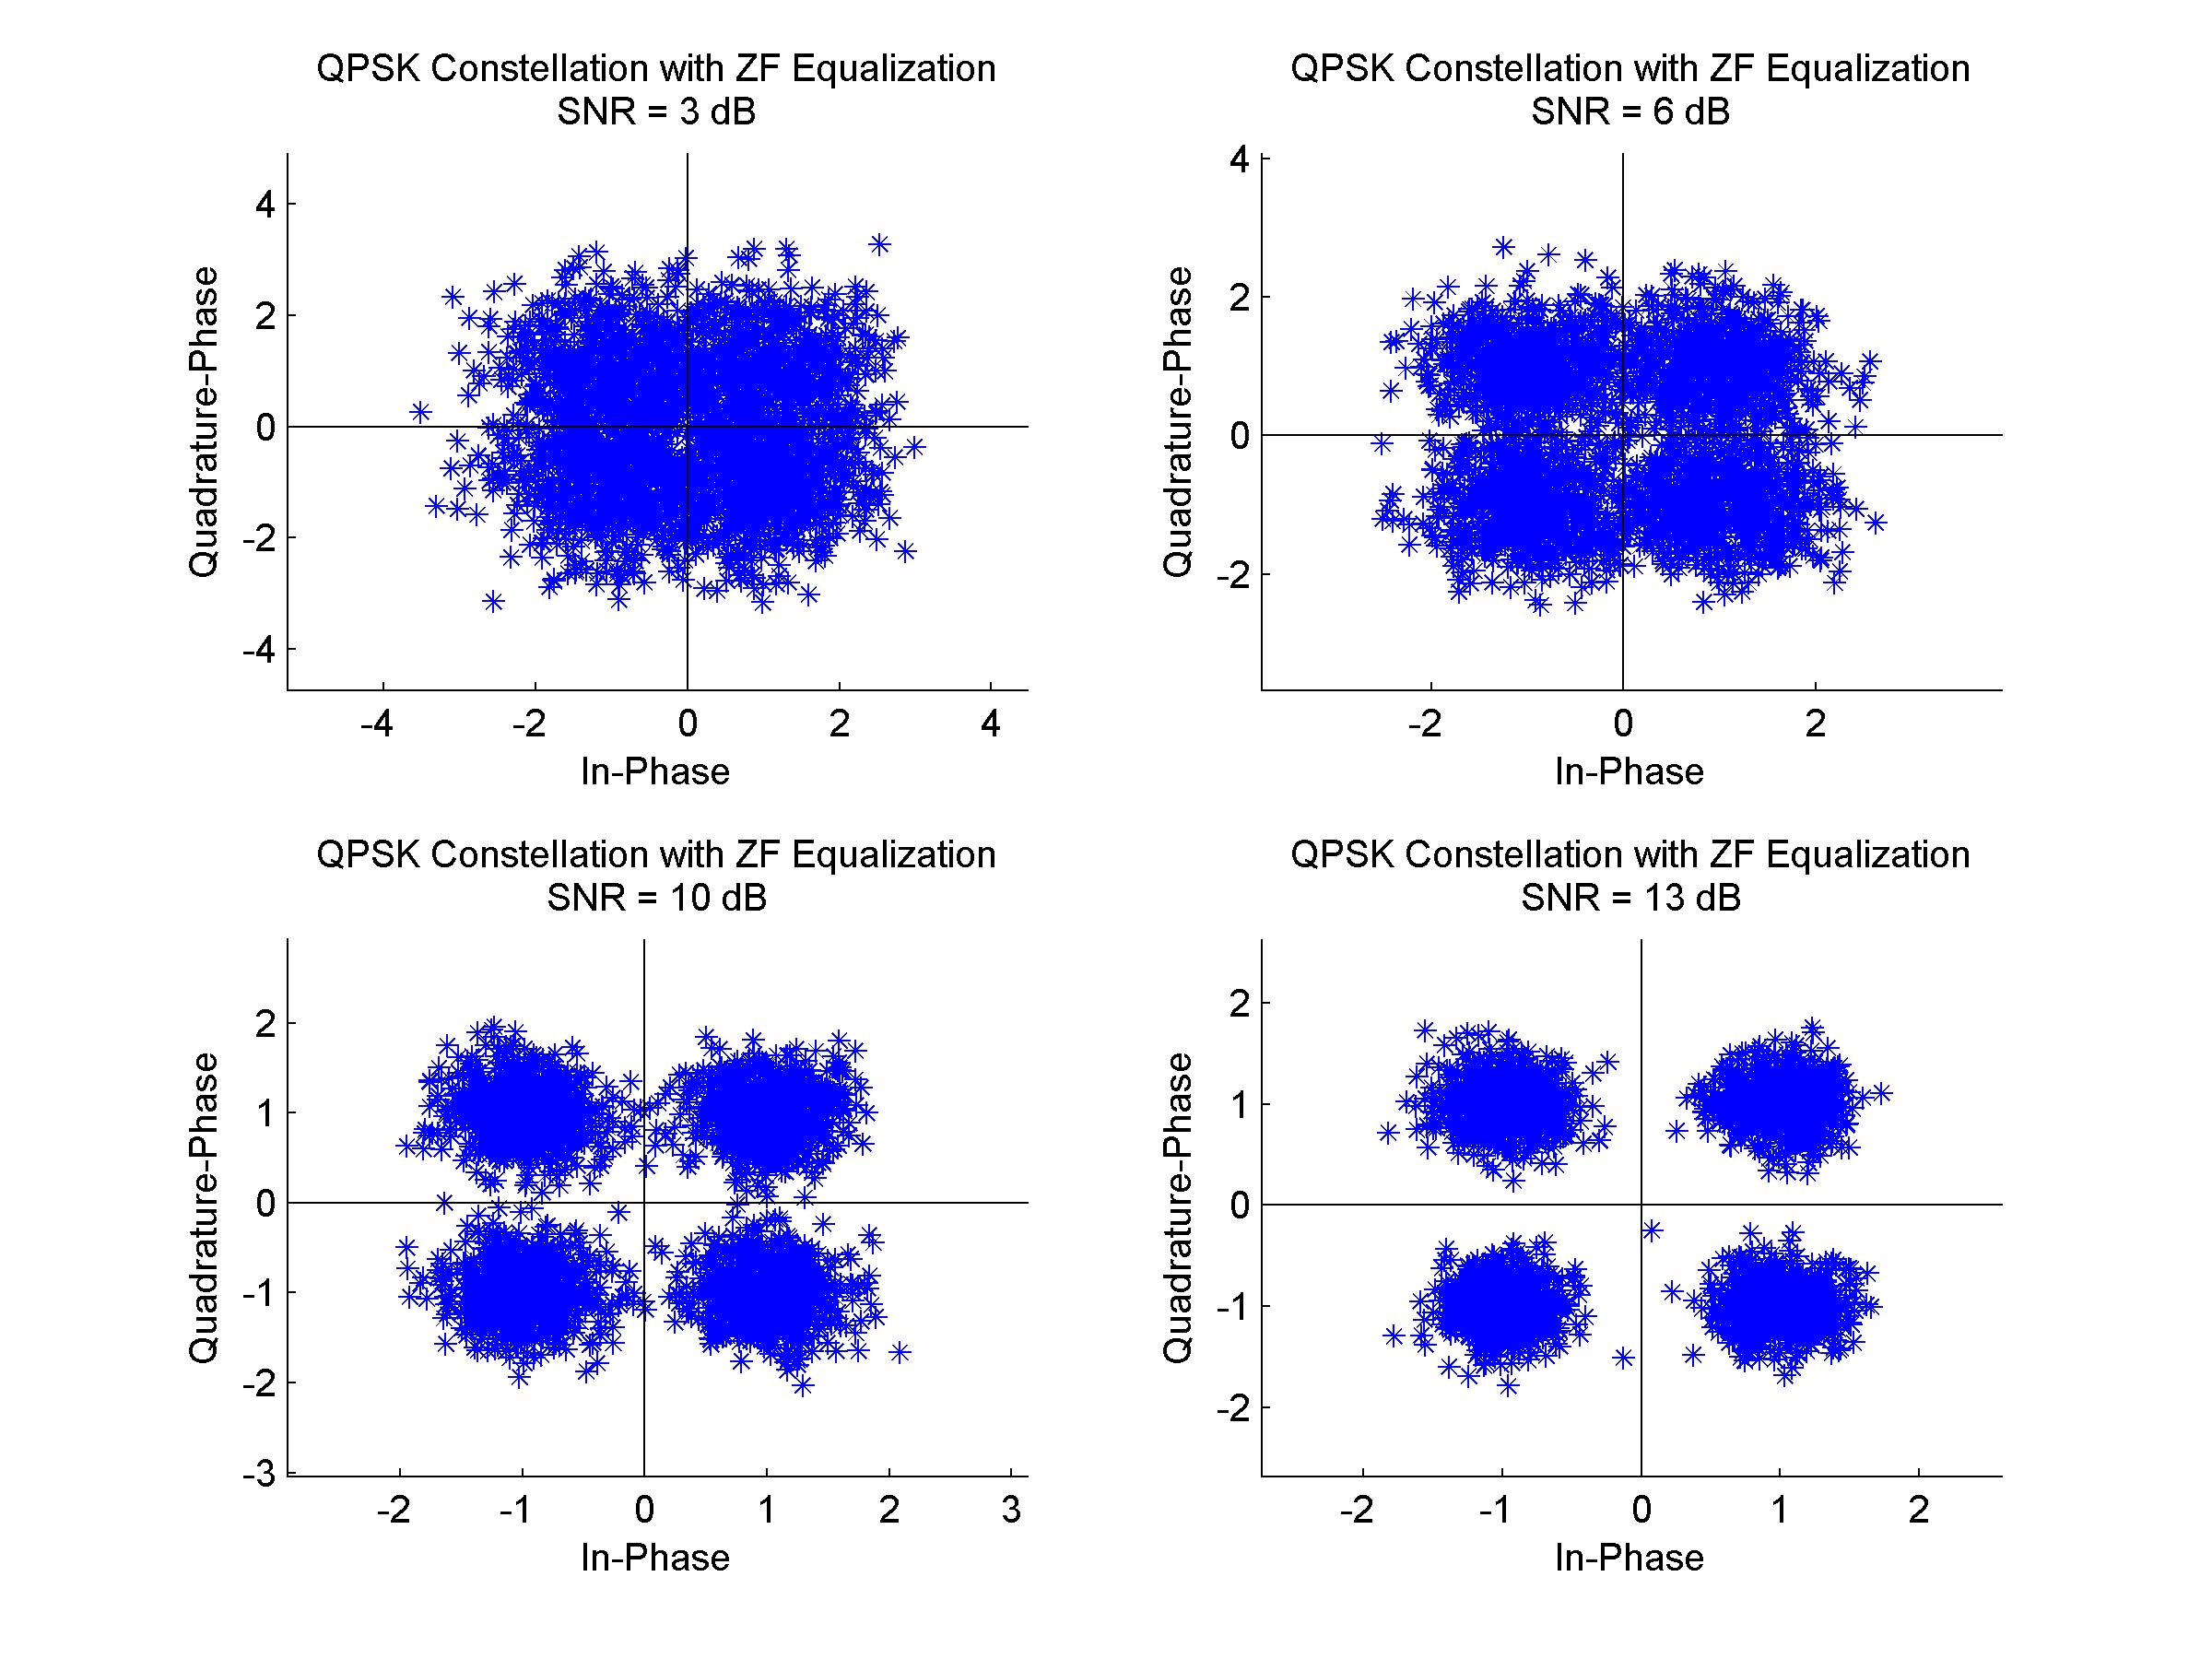
\includegraphics[width=0.7\textwidth]{qpConstZF2.jpg}
\caption{Constellation plot for a QPSK modulated signal with ZF equalization under channel reponse $h_2(t)$}
\end{figure}

\begin{figure}[H]
\centering
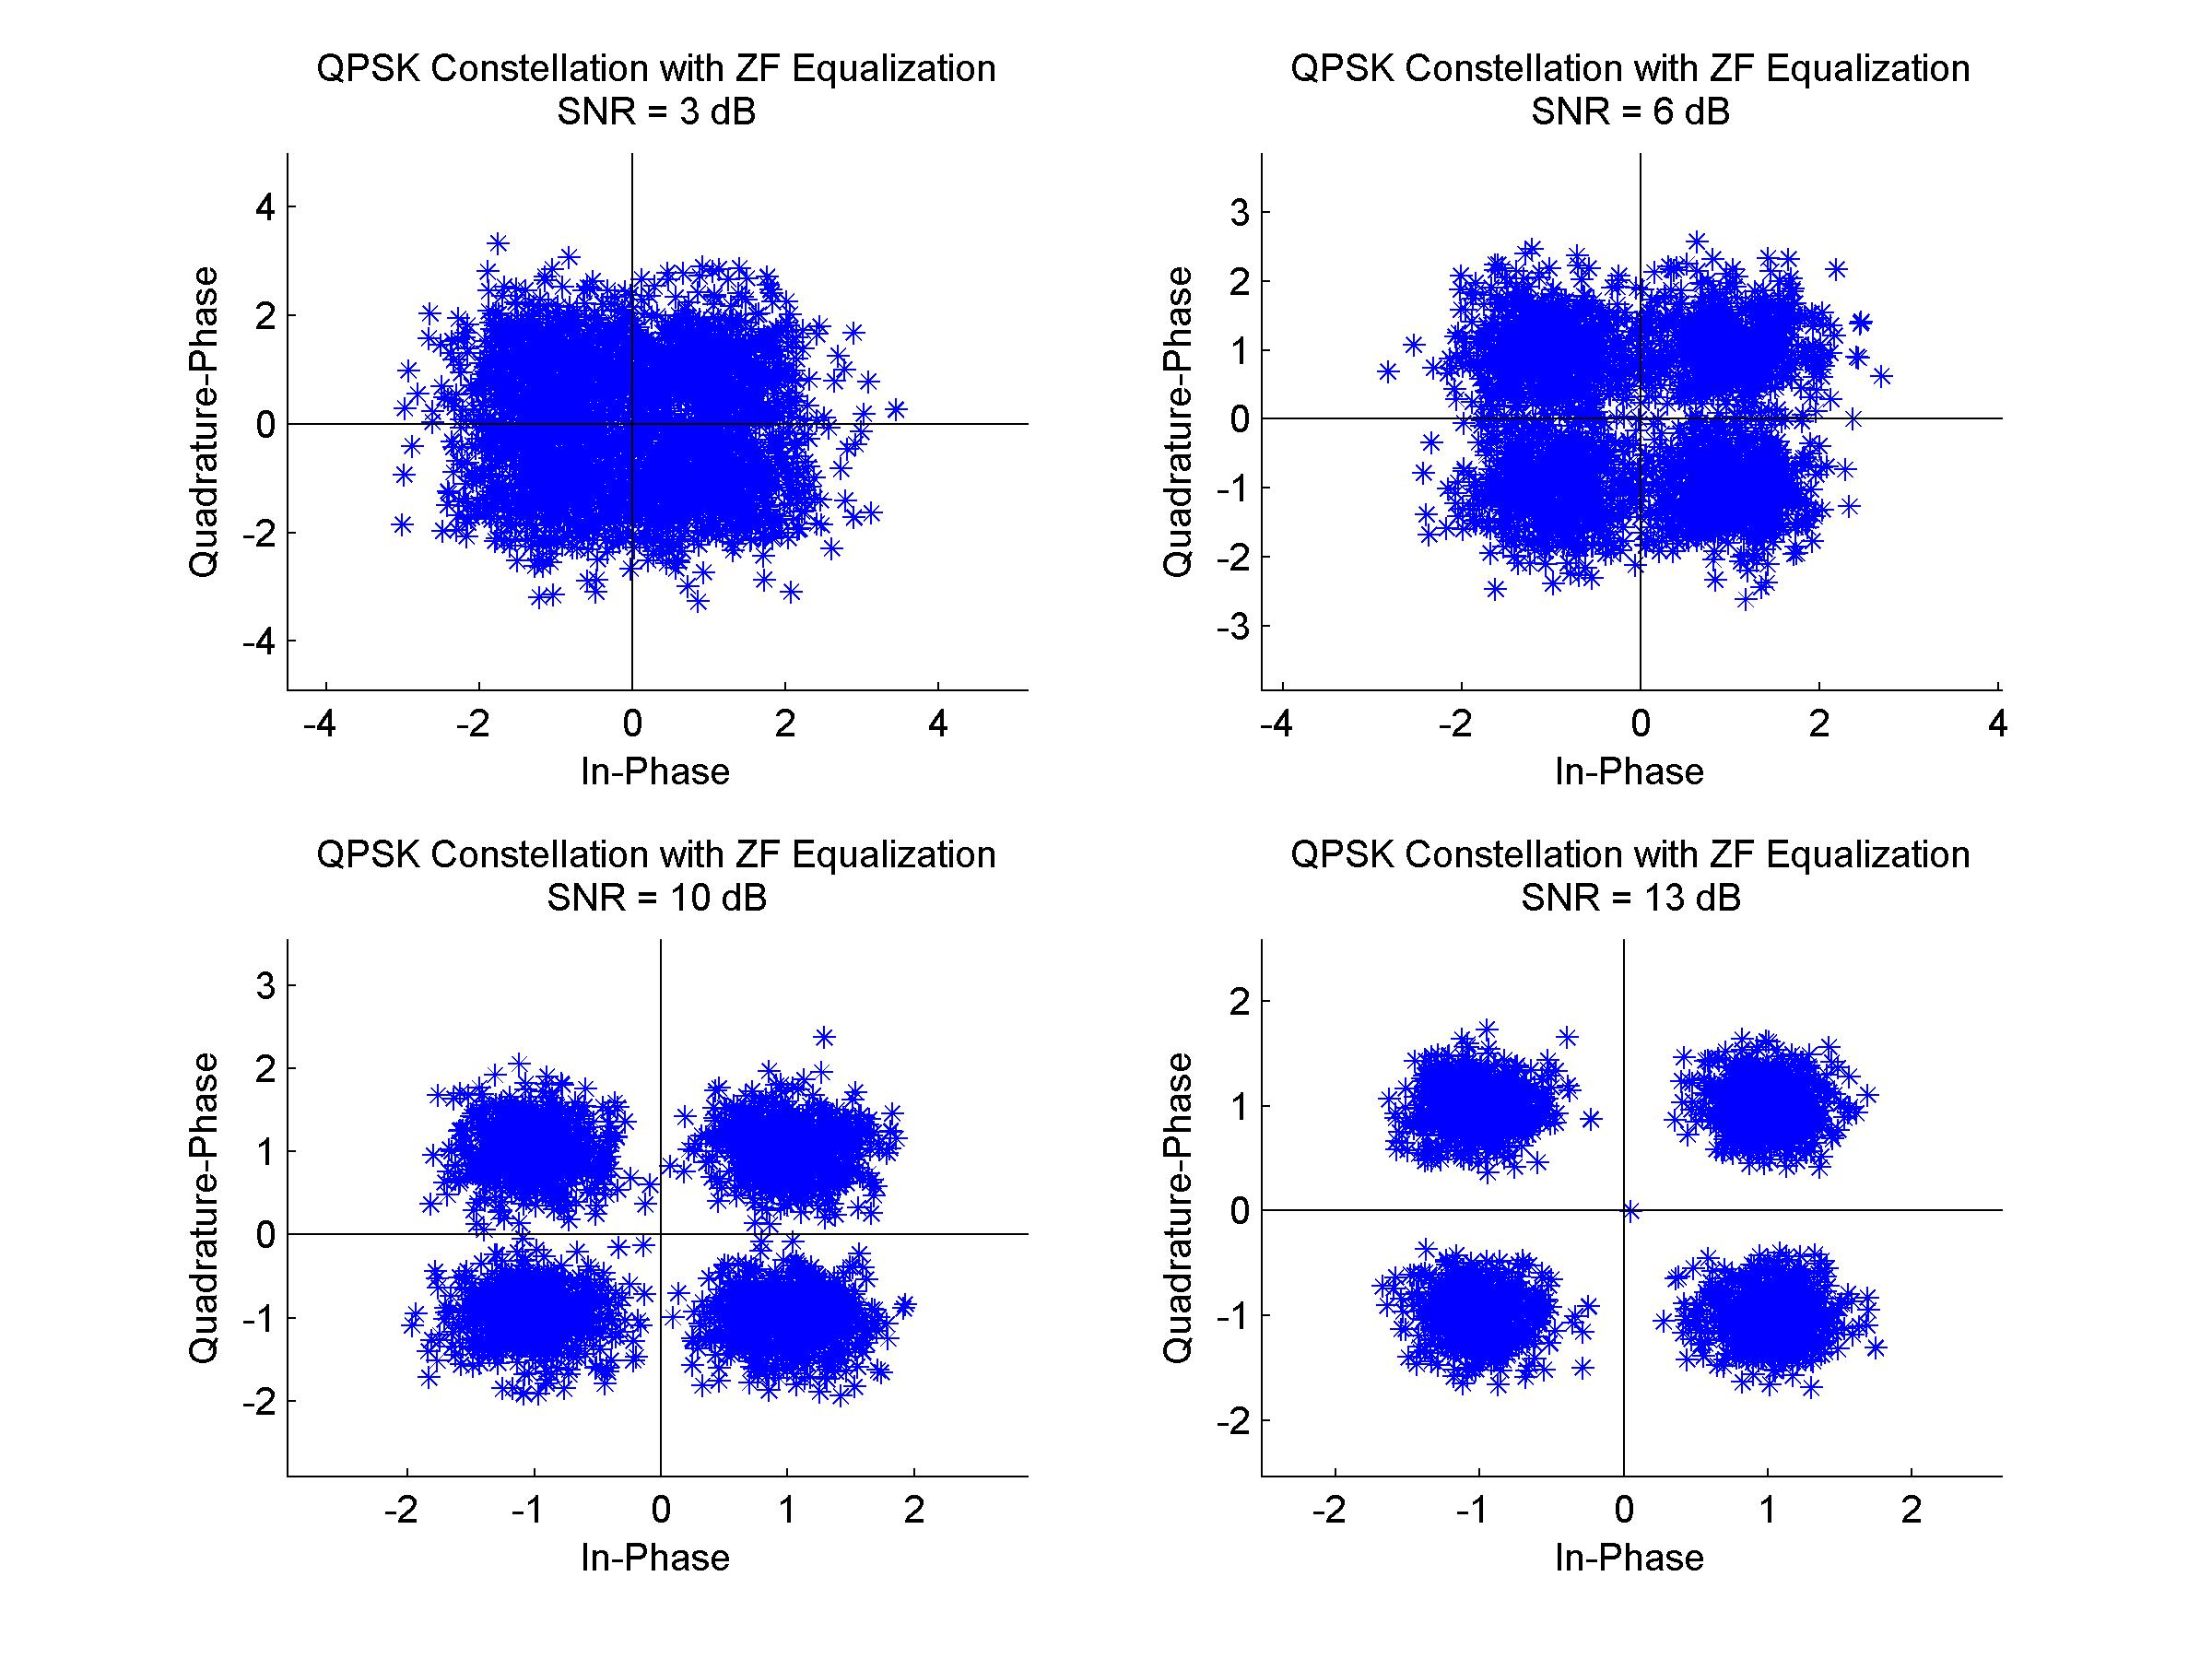
\includegraphics[width=0.7\textwidth]{qpConstZF3.jpg}
\caption{Constellation plot for a QPSK modulated signal with ZF equalization under channel reponse $h_3(t)$}
\end{figure}

\subsubsection{BPSK with MMSE Equalization}

\begin{figure}[H]
\centering
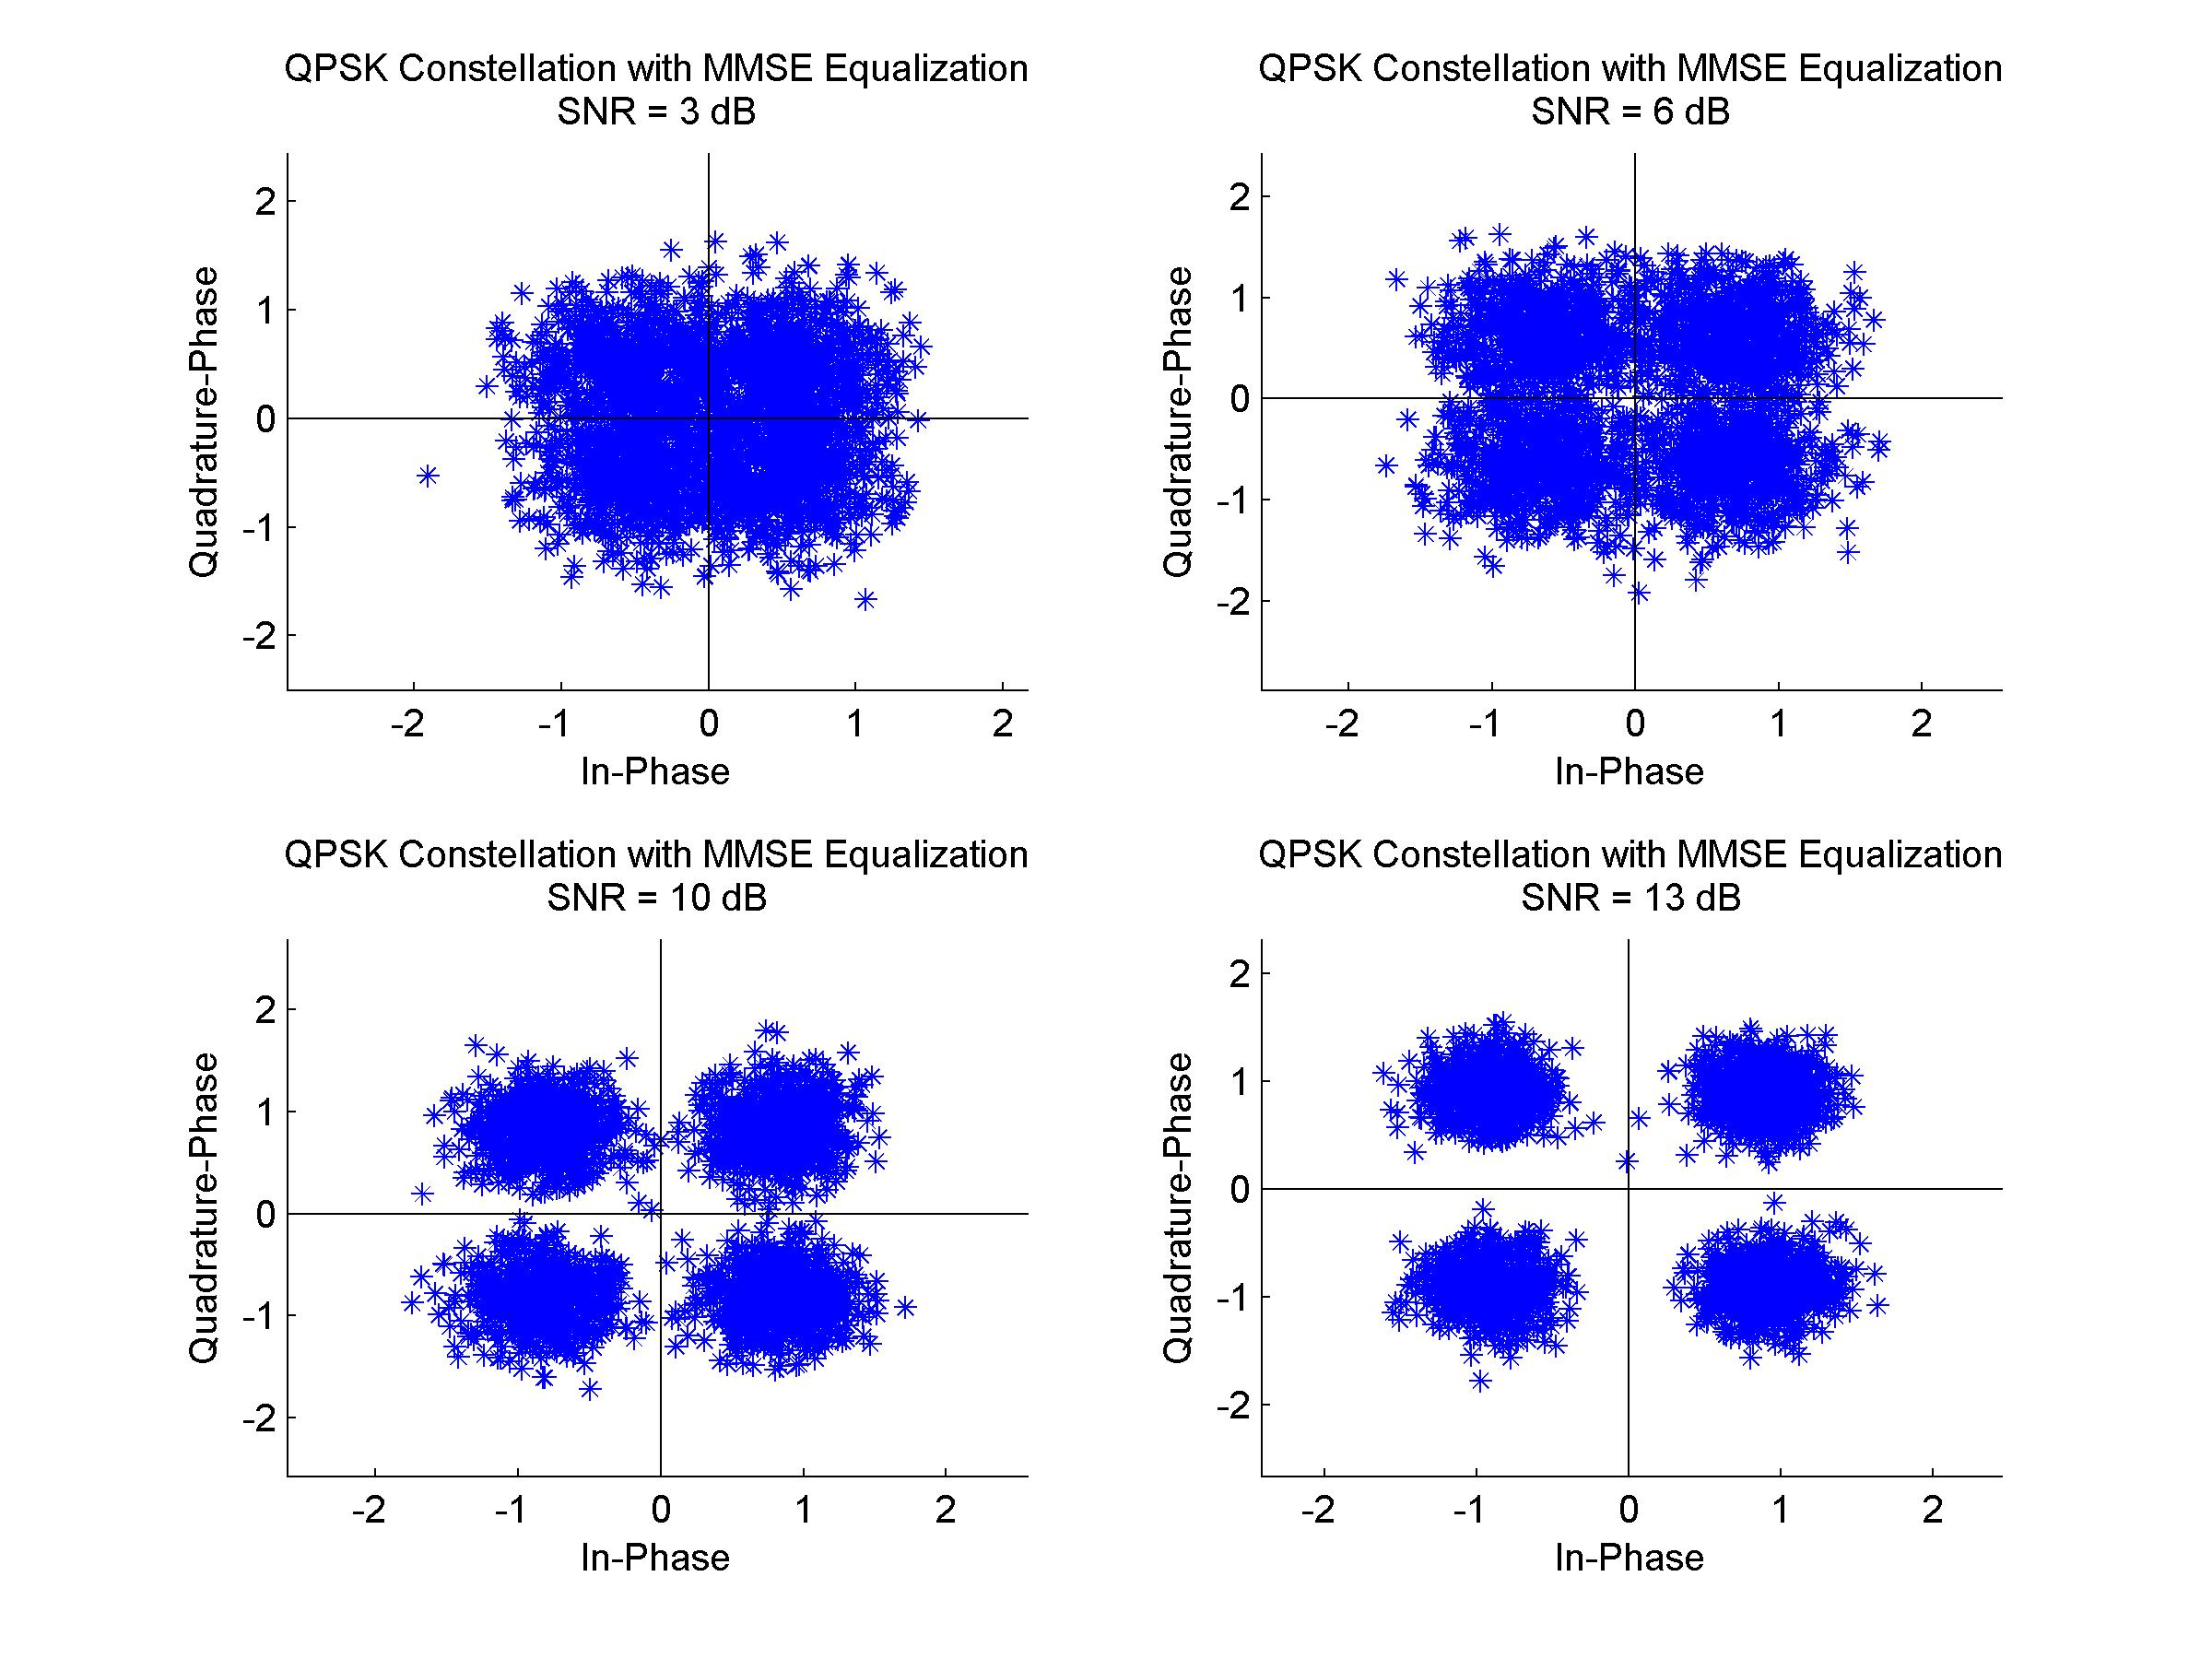
\includegraphics[width=0.7\textwidth]{qpConstMMSE1.jpg}
\caption{Constellation plot for a QPSK modulated signal with MMSE equalization under channel reponse $h_1(t)$}
\end{figure}

\begin{figure}[H]
\centering
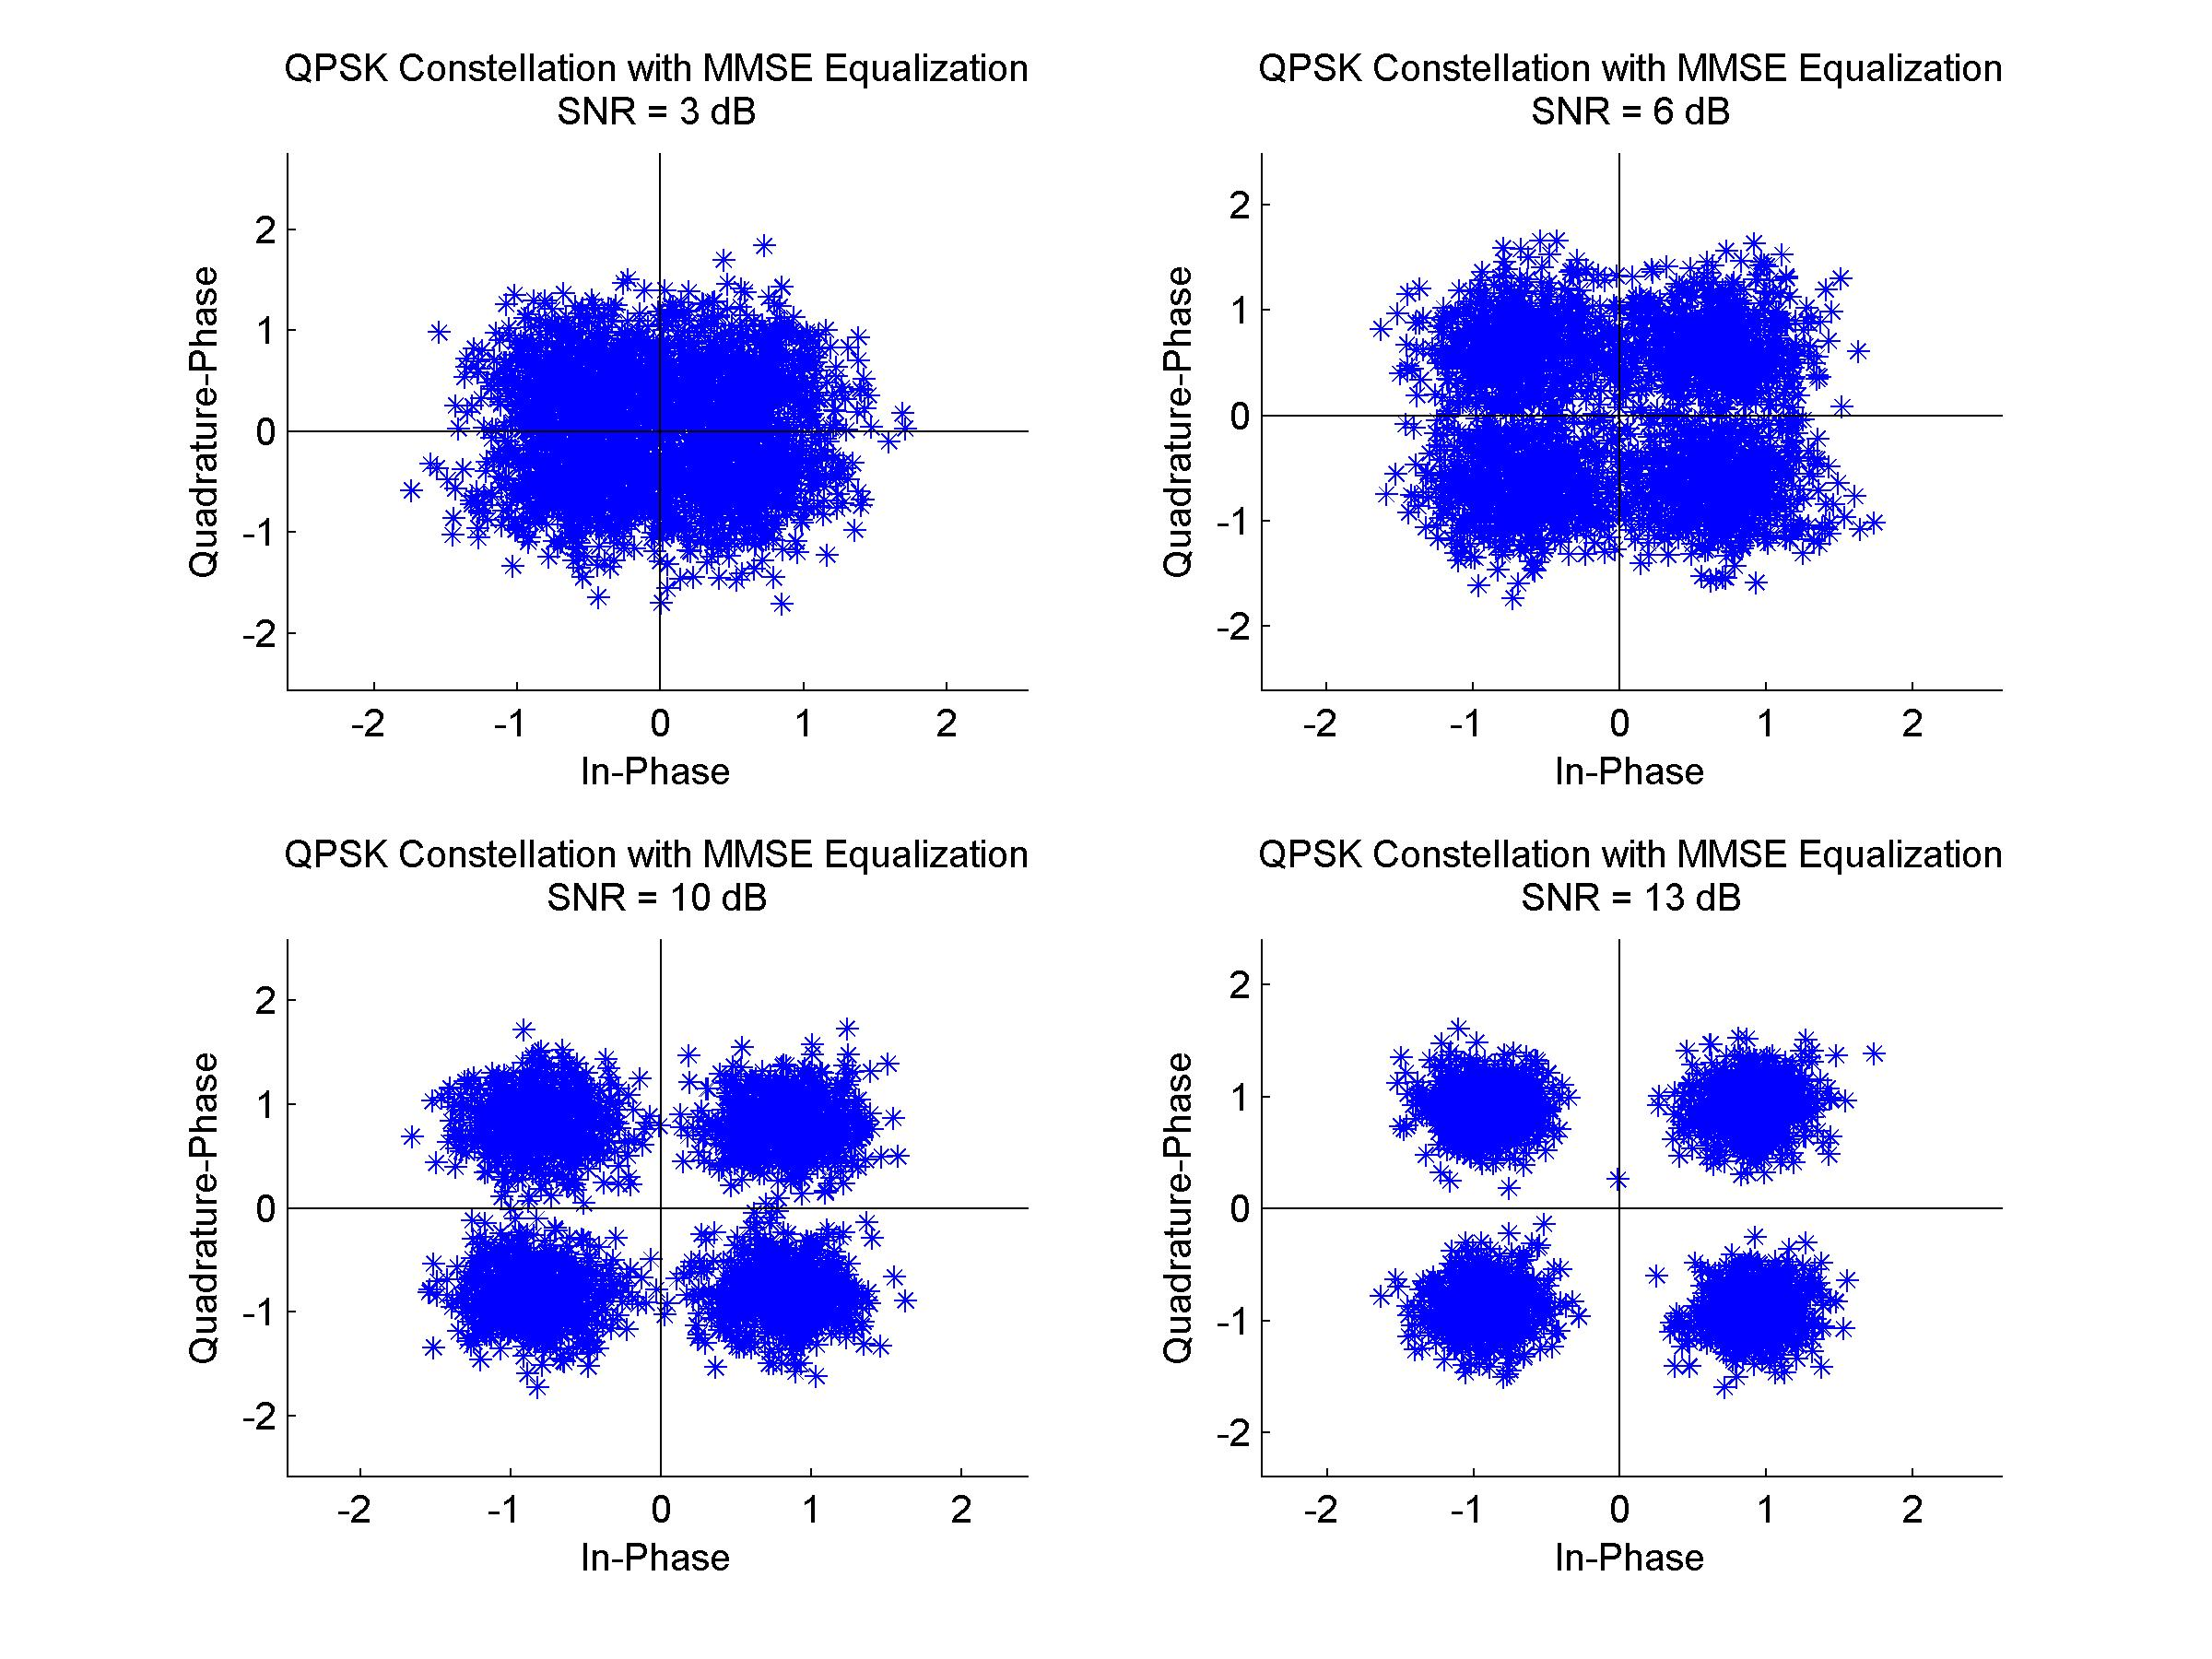
\includegraphics[width=0.7\textwidth]{qpConstMMSE2.jpg}
\caption{Constellation plot for a QPSK modulated signal with MMSE equalization under channel reponse $h_2(t)$}
\end{figure}

\begin{figure}[H]
\centering
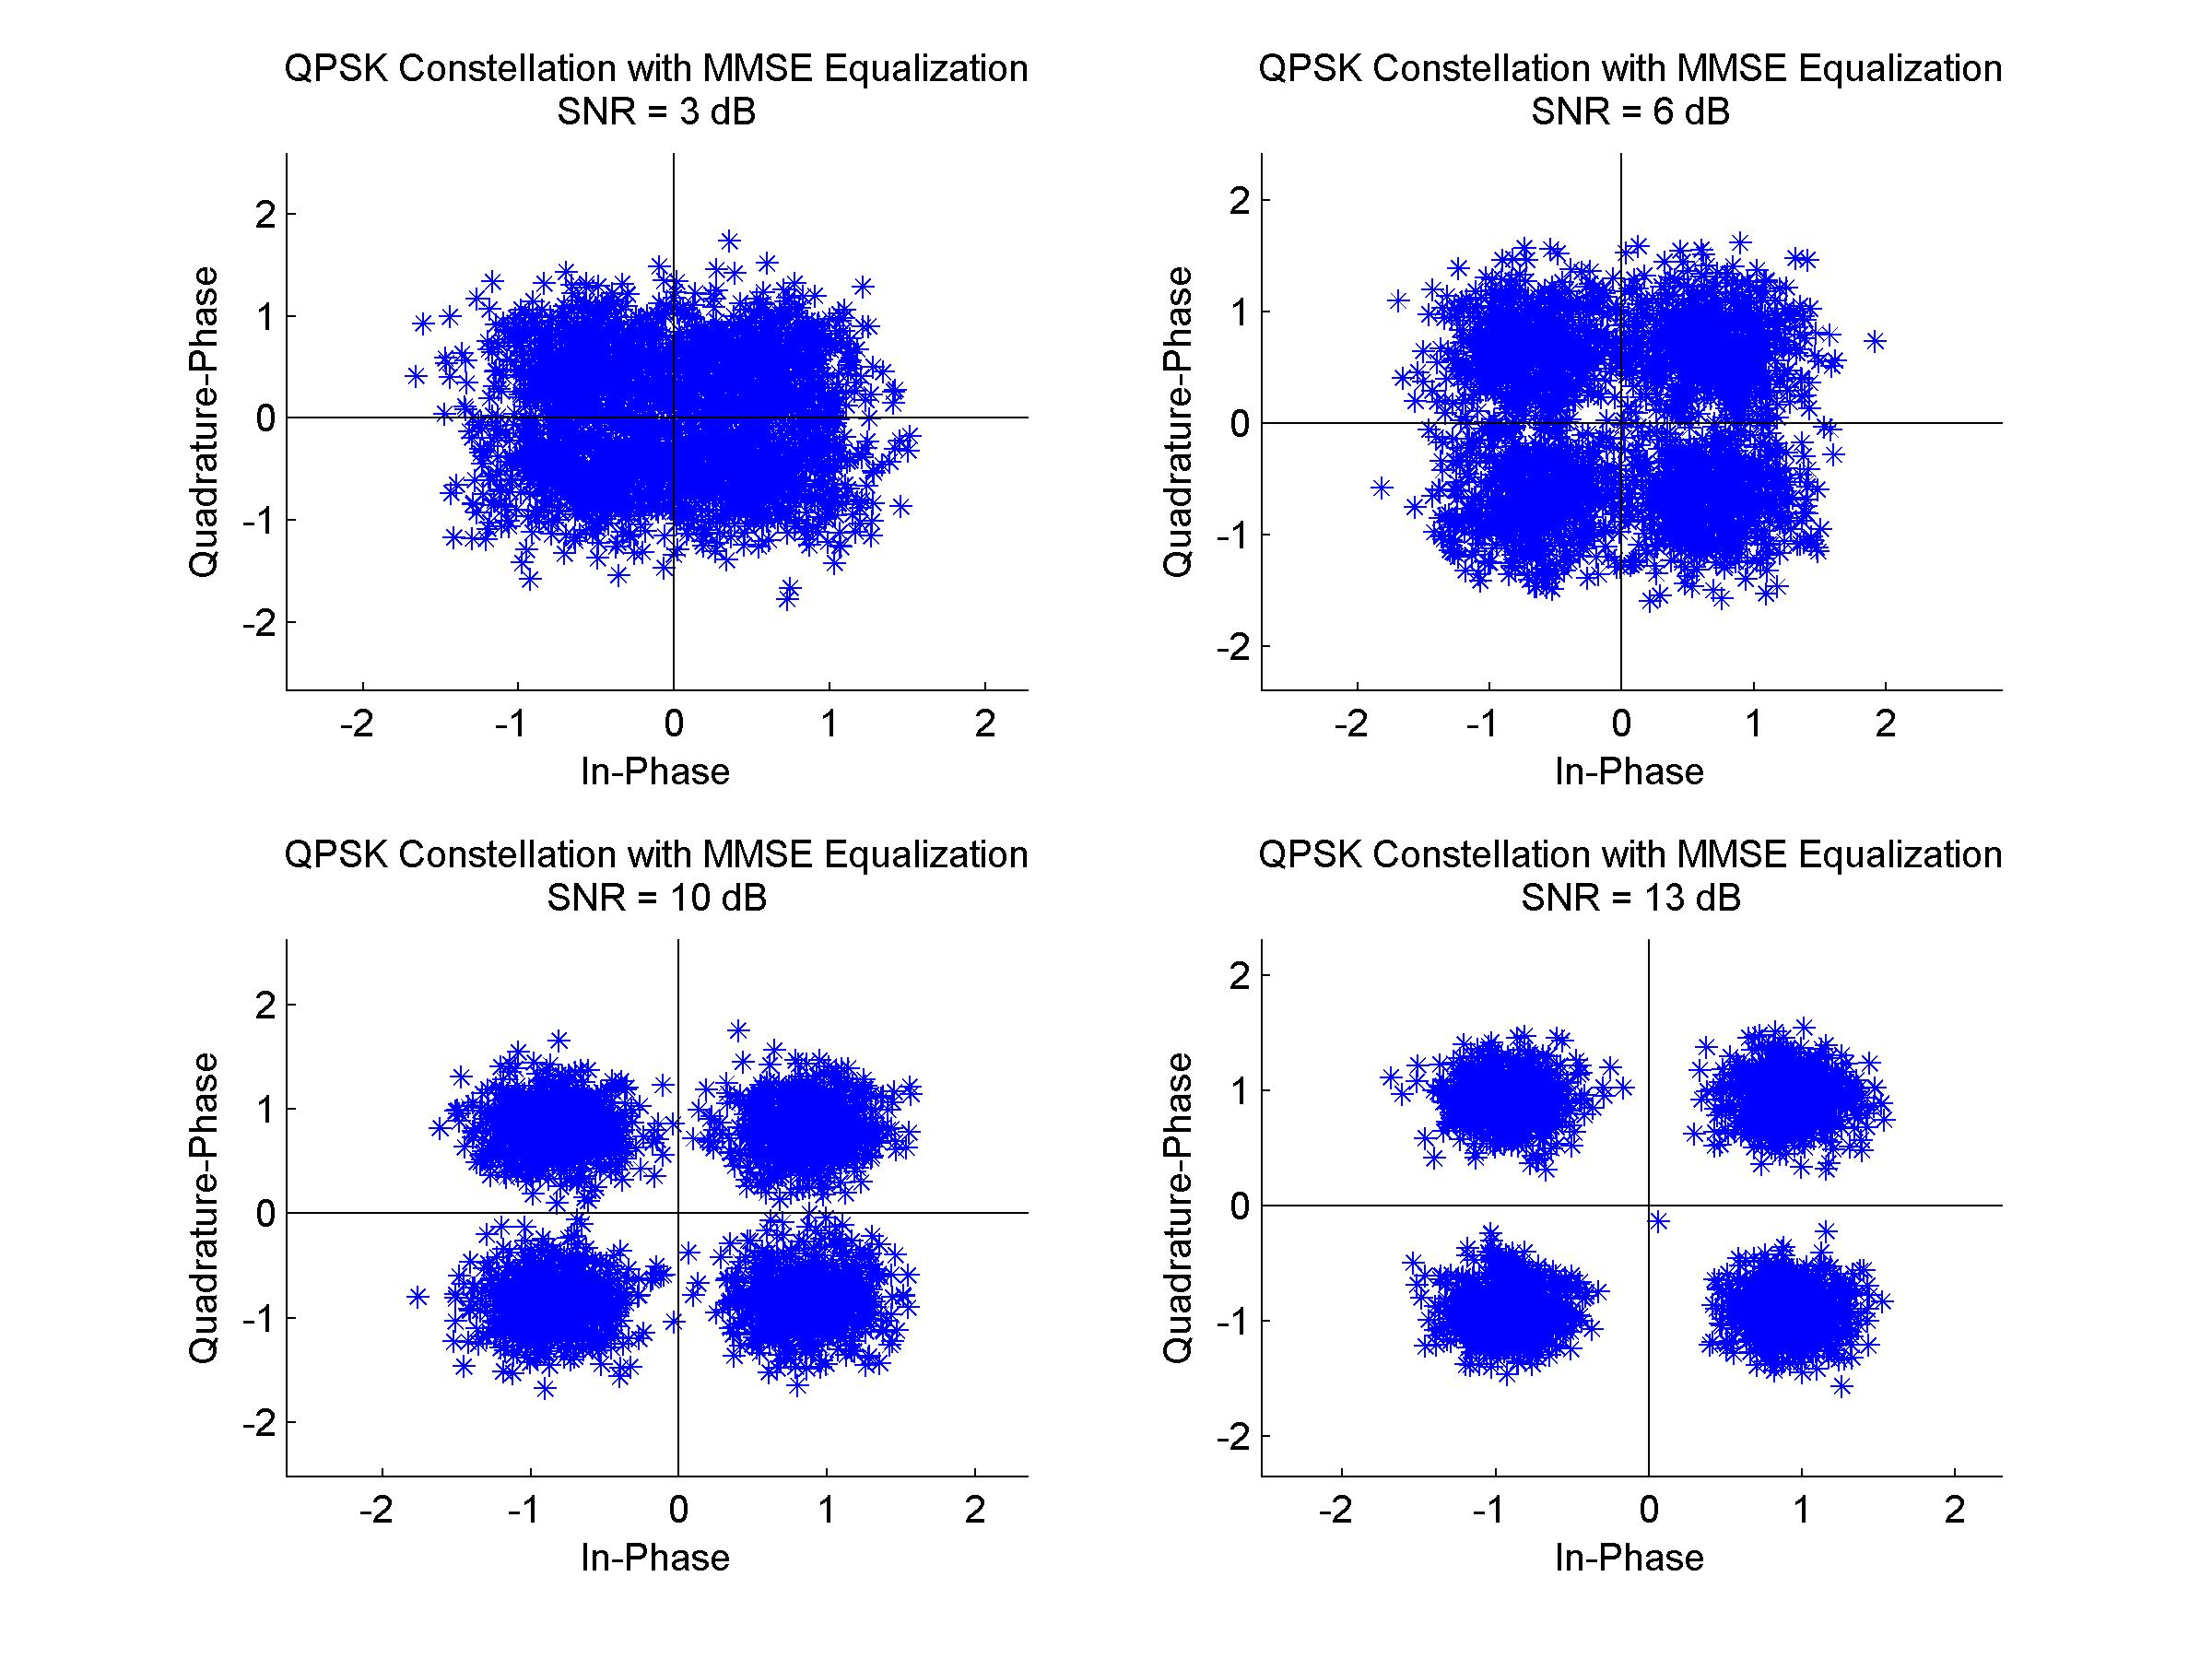
\includegraphics[width=0.7\textwidth]{qpConstMMSE3.jpg}
\caption{Constellation plot for a QPSK modulated signal with MMSE equalization under channel reponse $h_3(t)$}
\end{figure}

\subsubsection{QPSK with MMSE-DFE Equalization}

\begin{figure}[H]
\centering
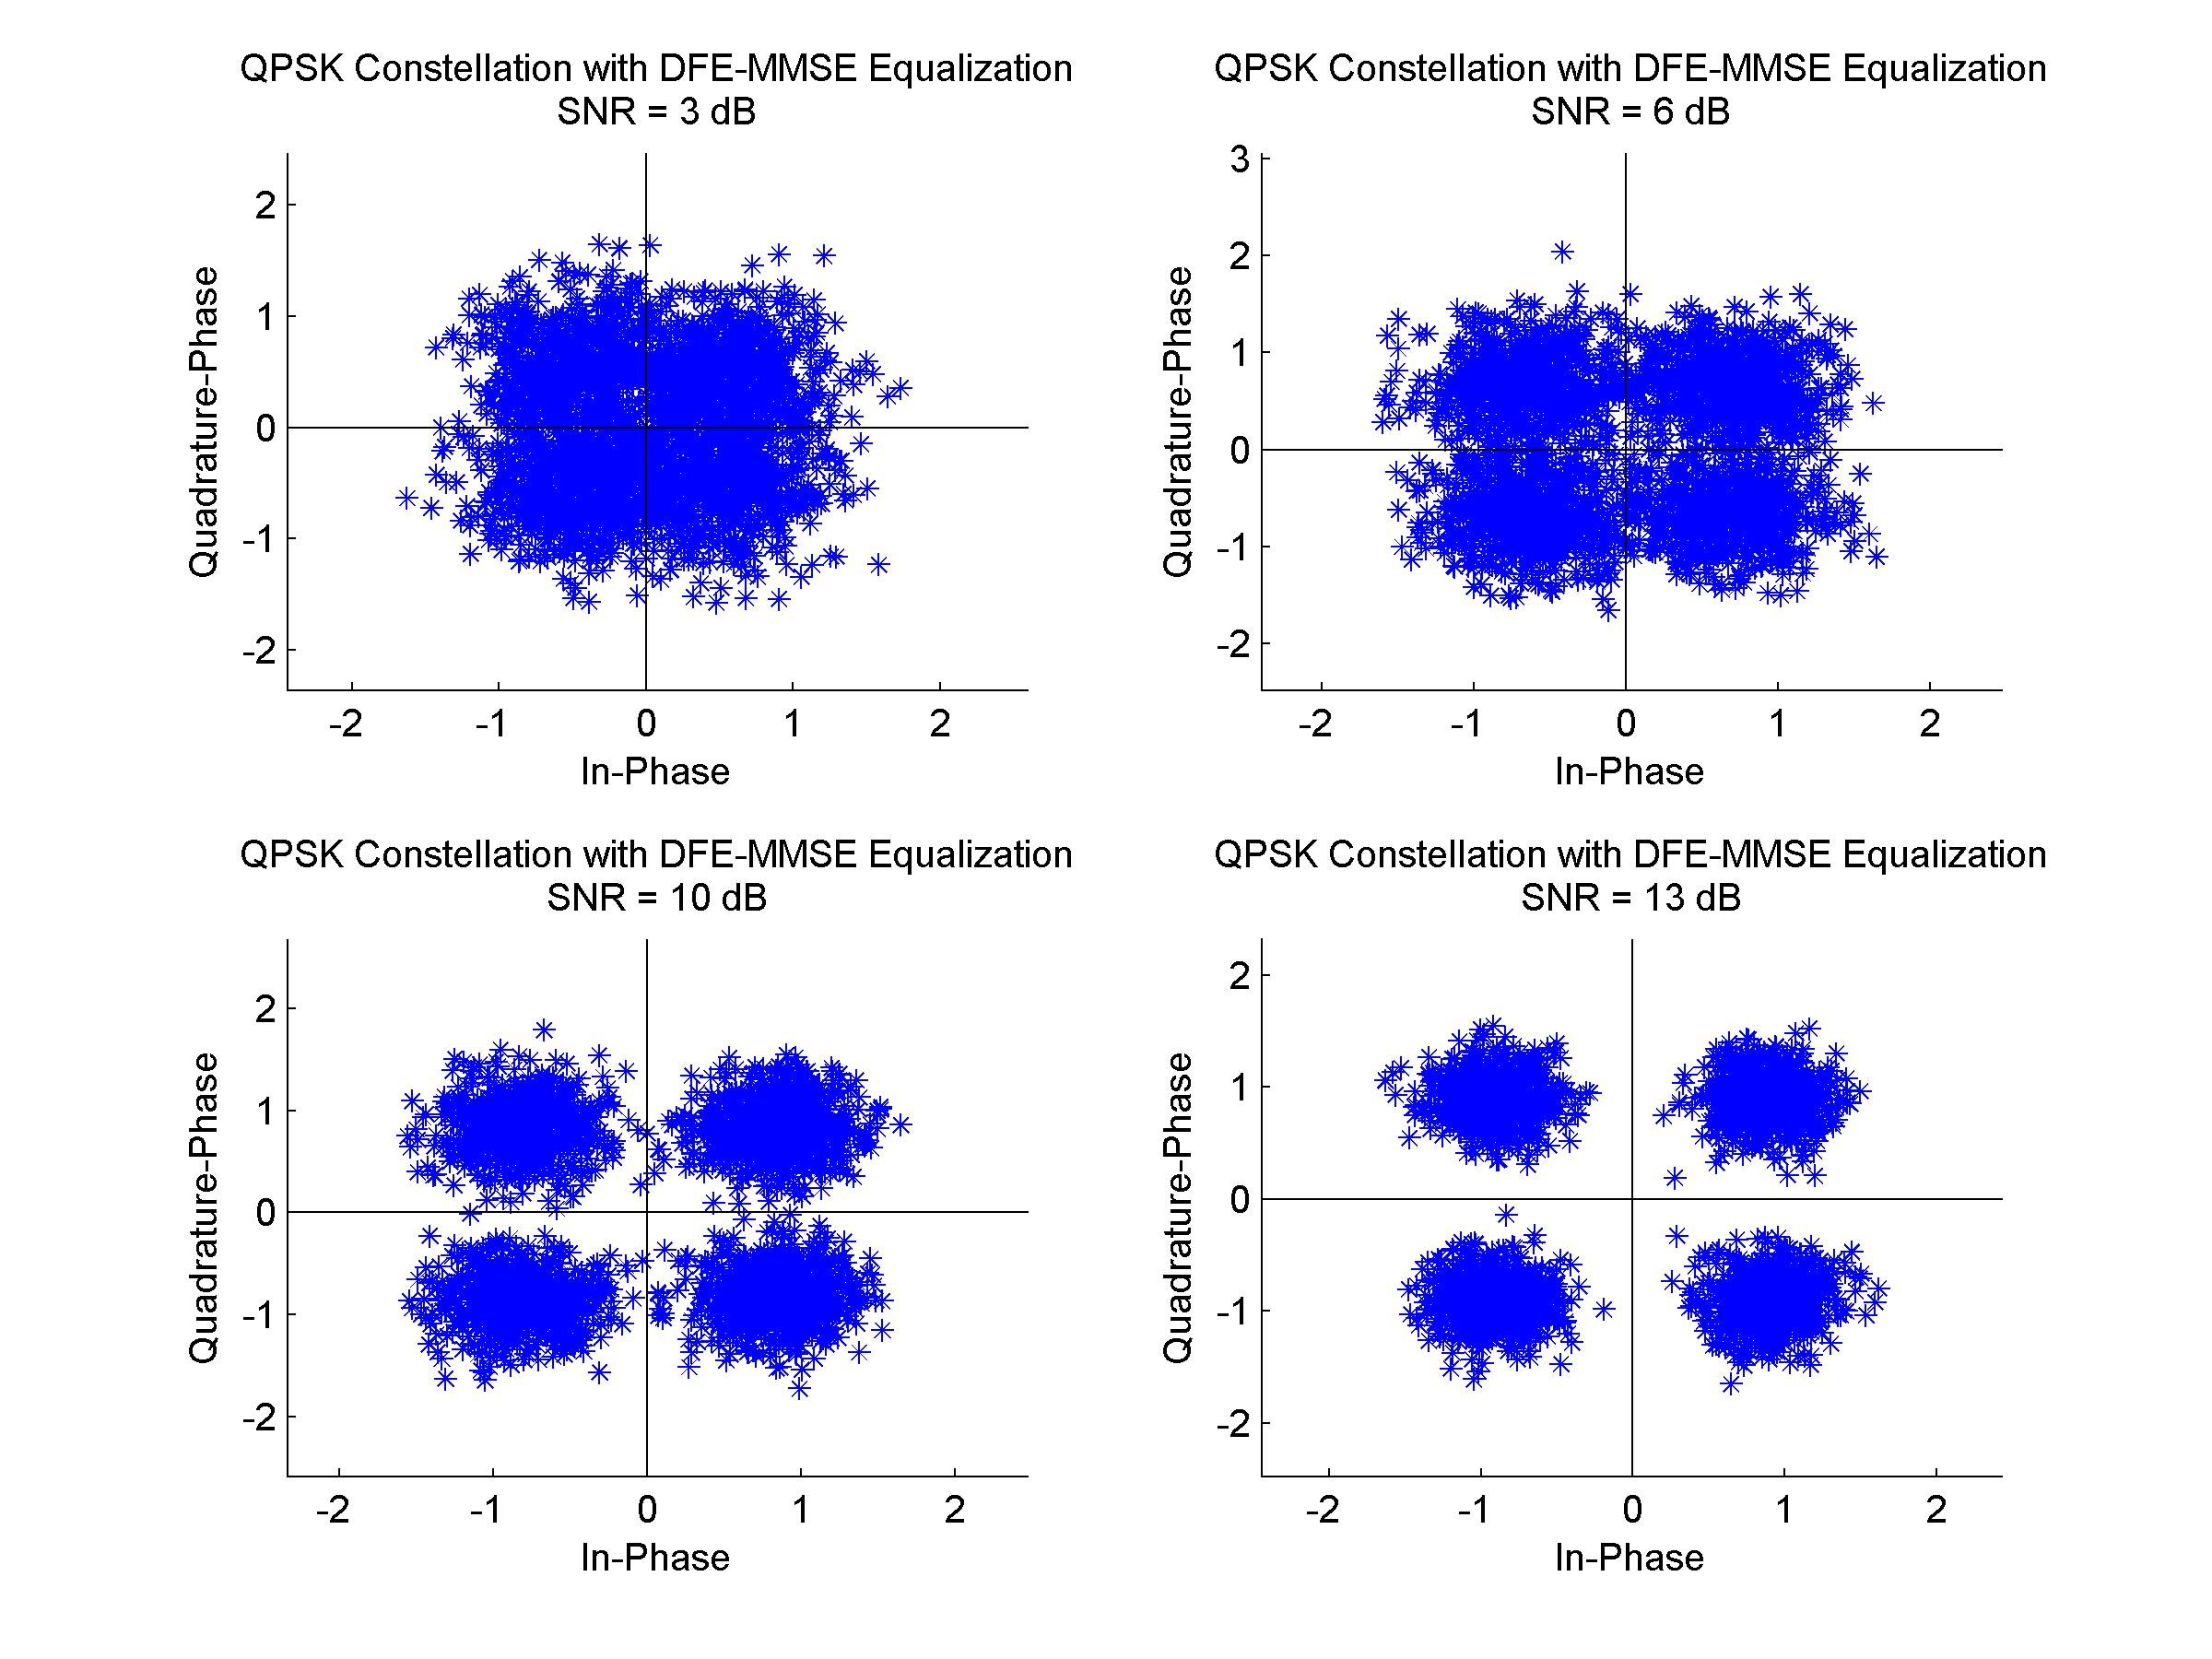
\includegraphics[width=0.7\textwidth]{qpConstDFEMMSE1.jpg}
\caption{Constellation plot for a QPSK modulated signal with MMSE-DFE equalization under channel reponse $h_1(t)$}
\end{figure}

\begin{figure}[H]
\centering
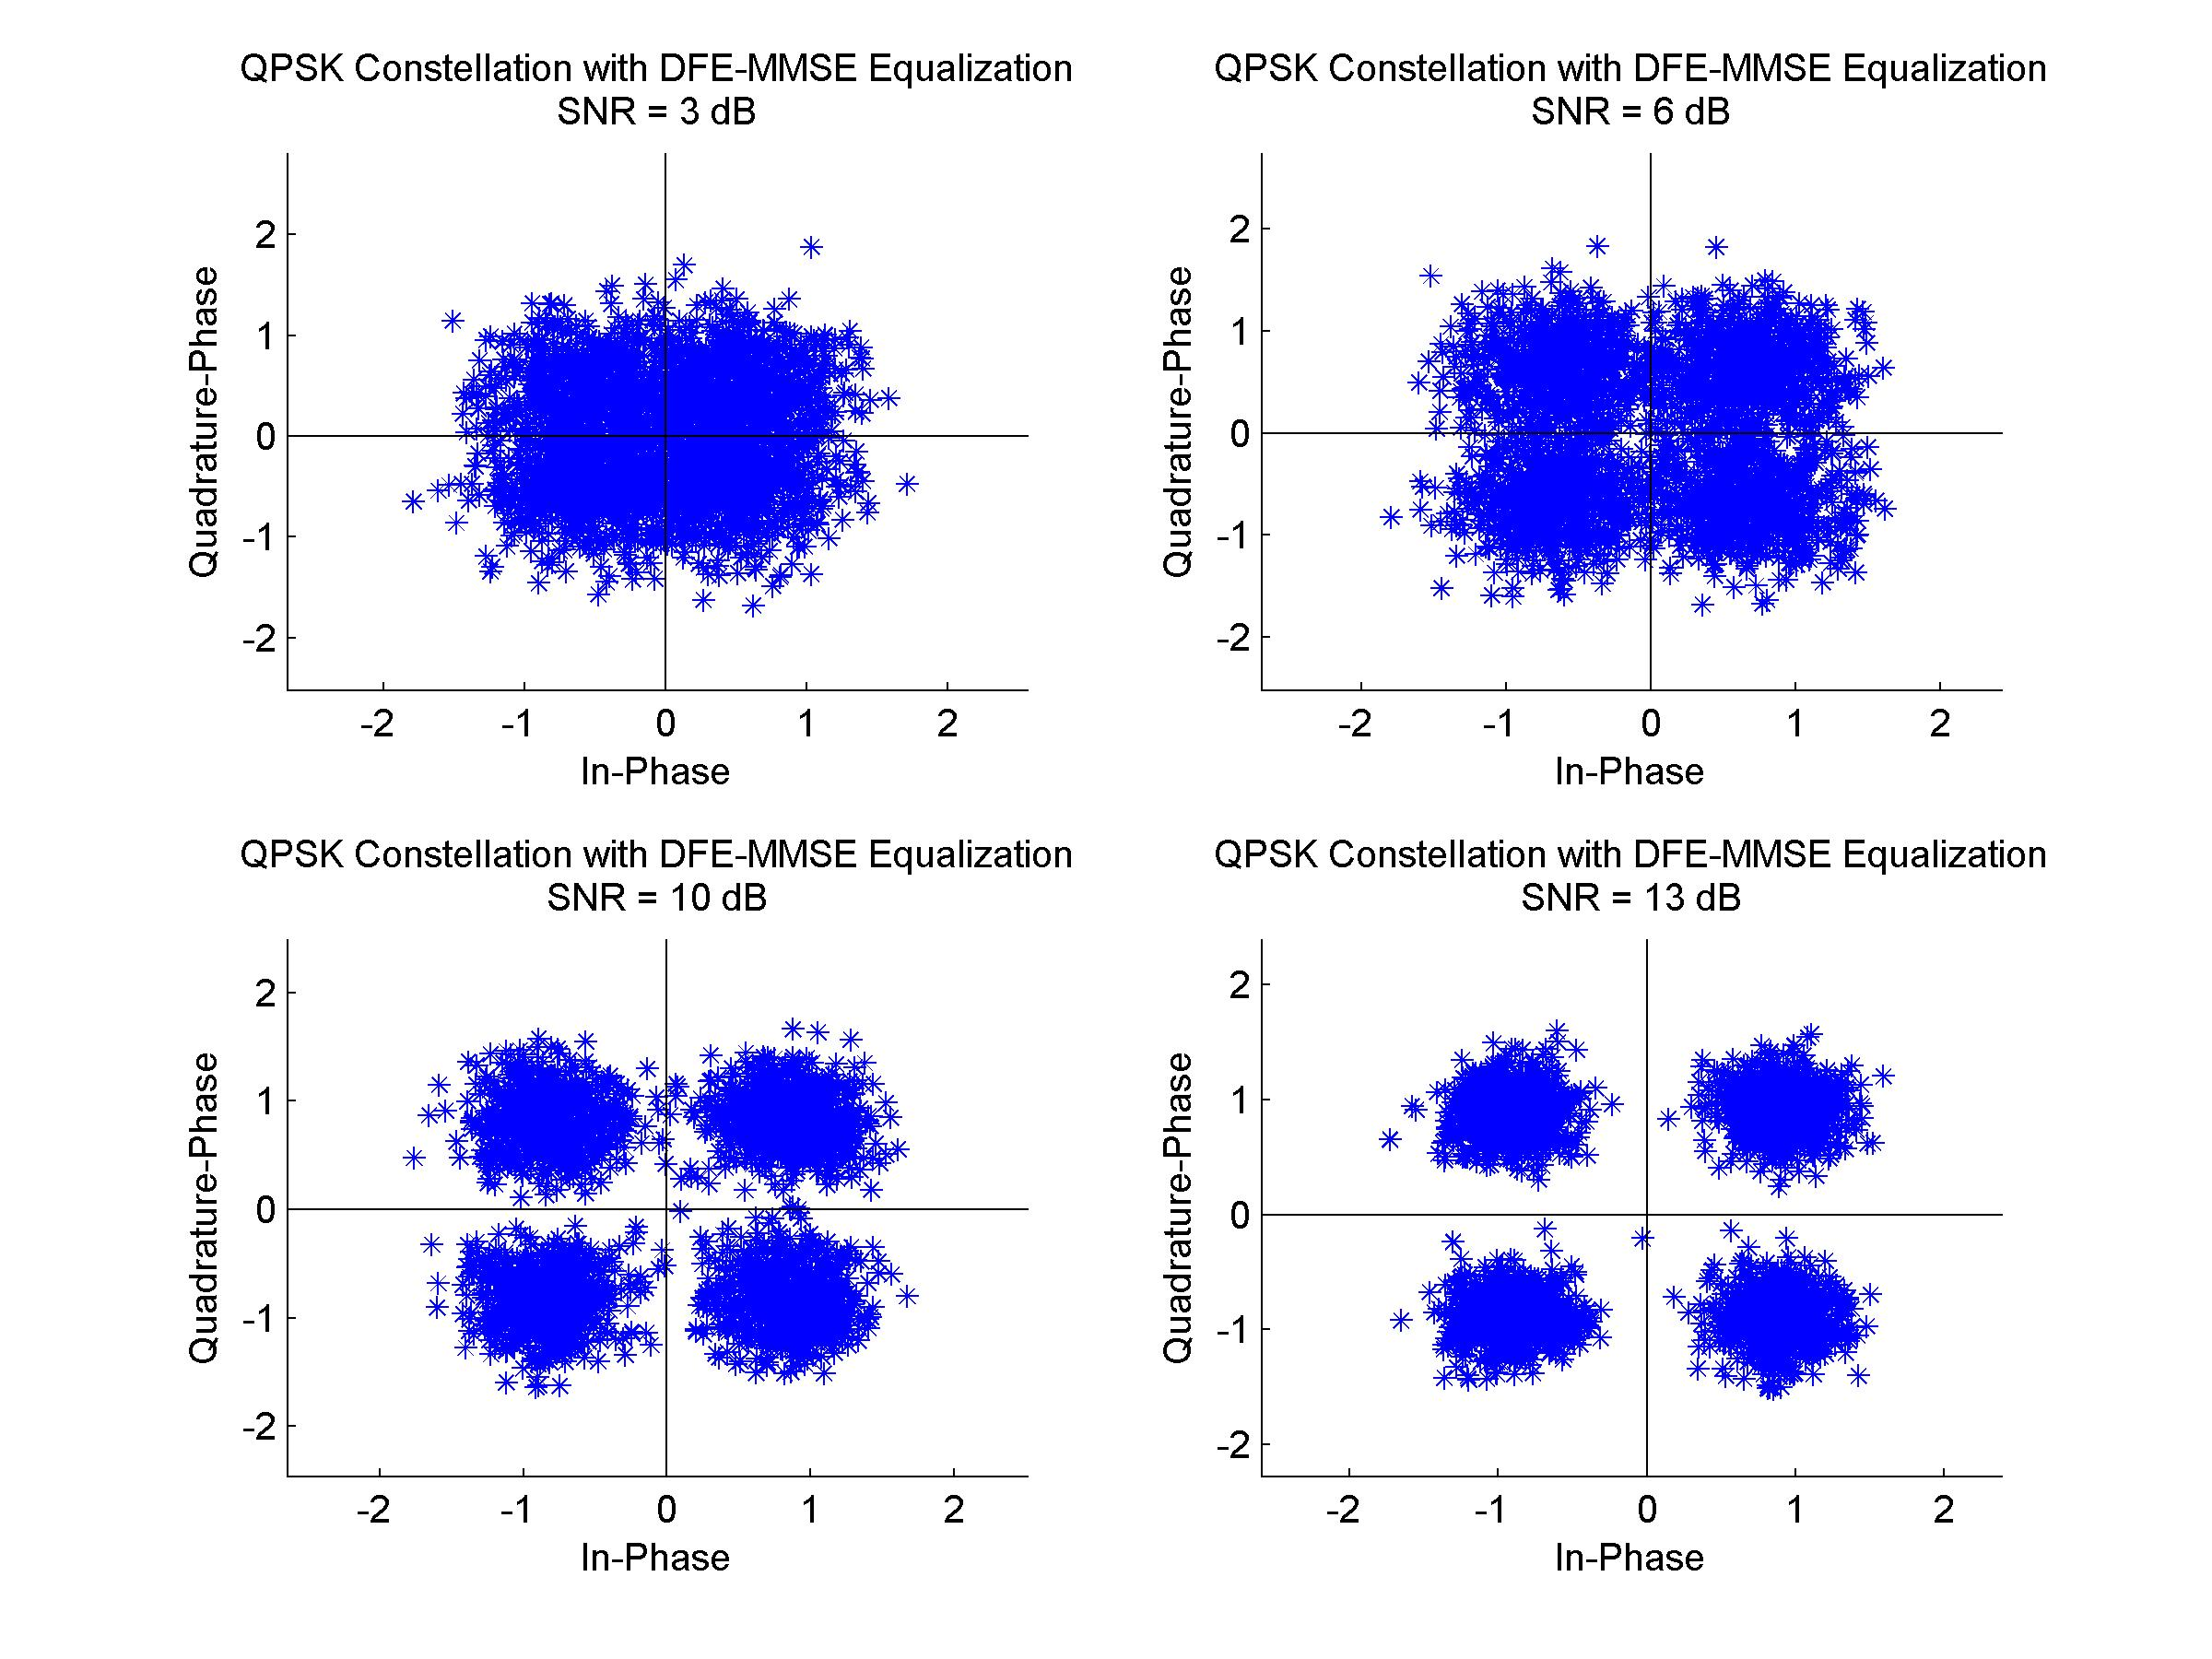
\includegraphics[width=0.7\textwidth]{qpConstDFEMMSE2.jpg}
\caption{Constellation plot for a QPSK modulated signal with MMSE-DFE equalization under channel reponse $h_2(t)$}
\end{figure}

\begin{figure}[H]
\centering
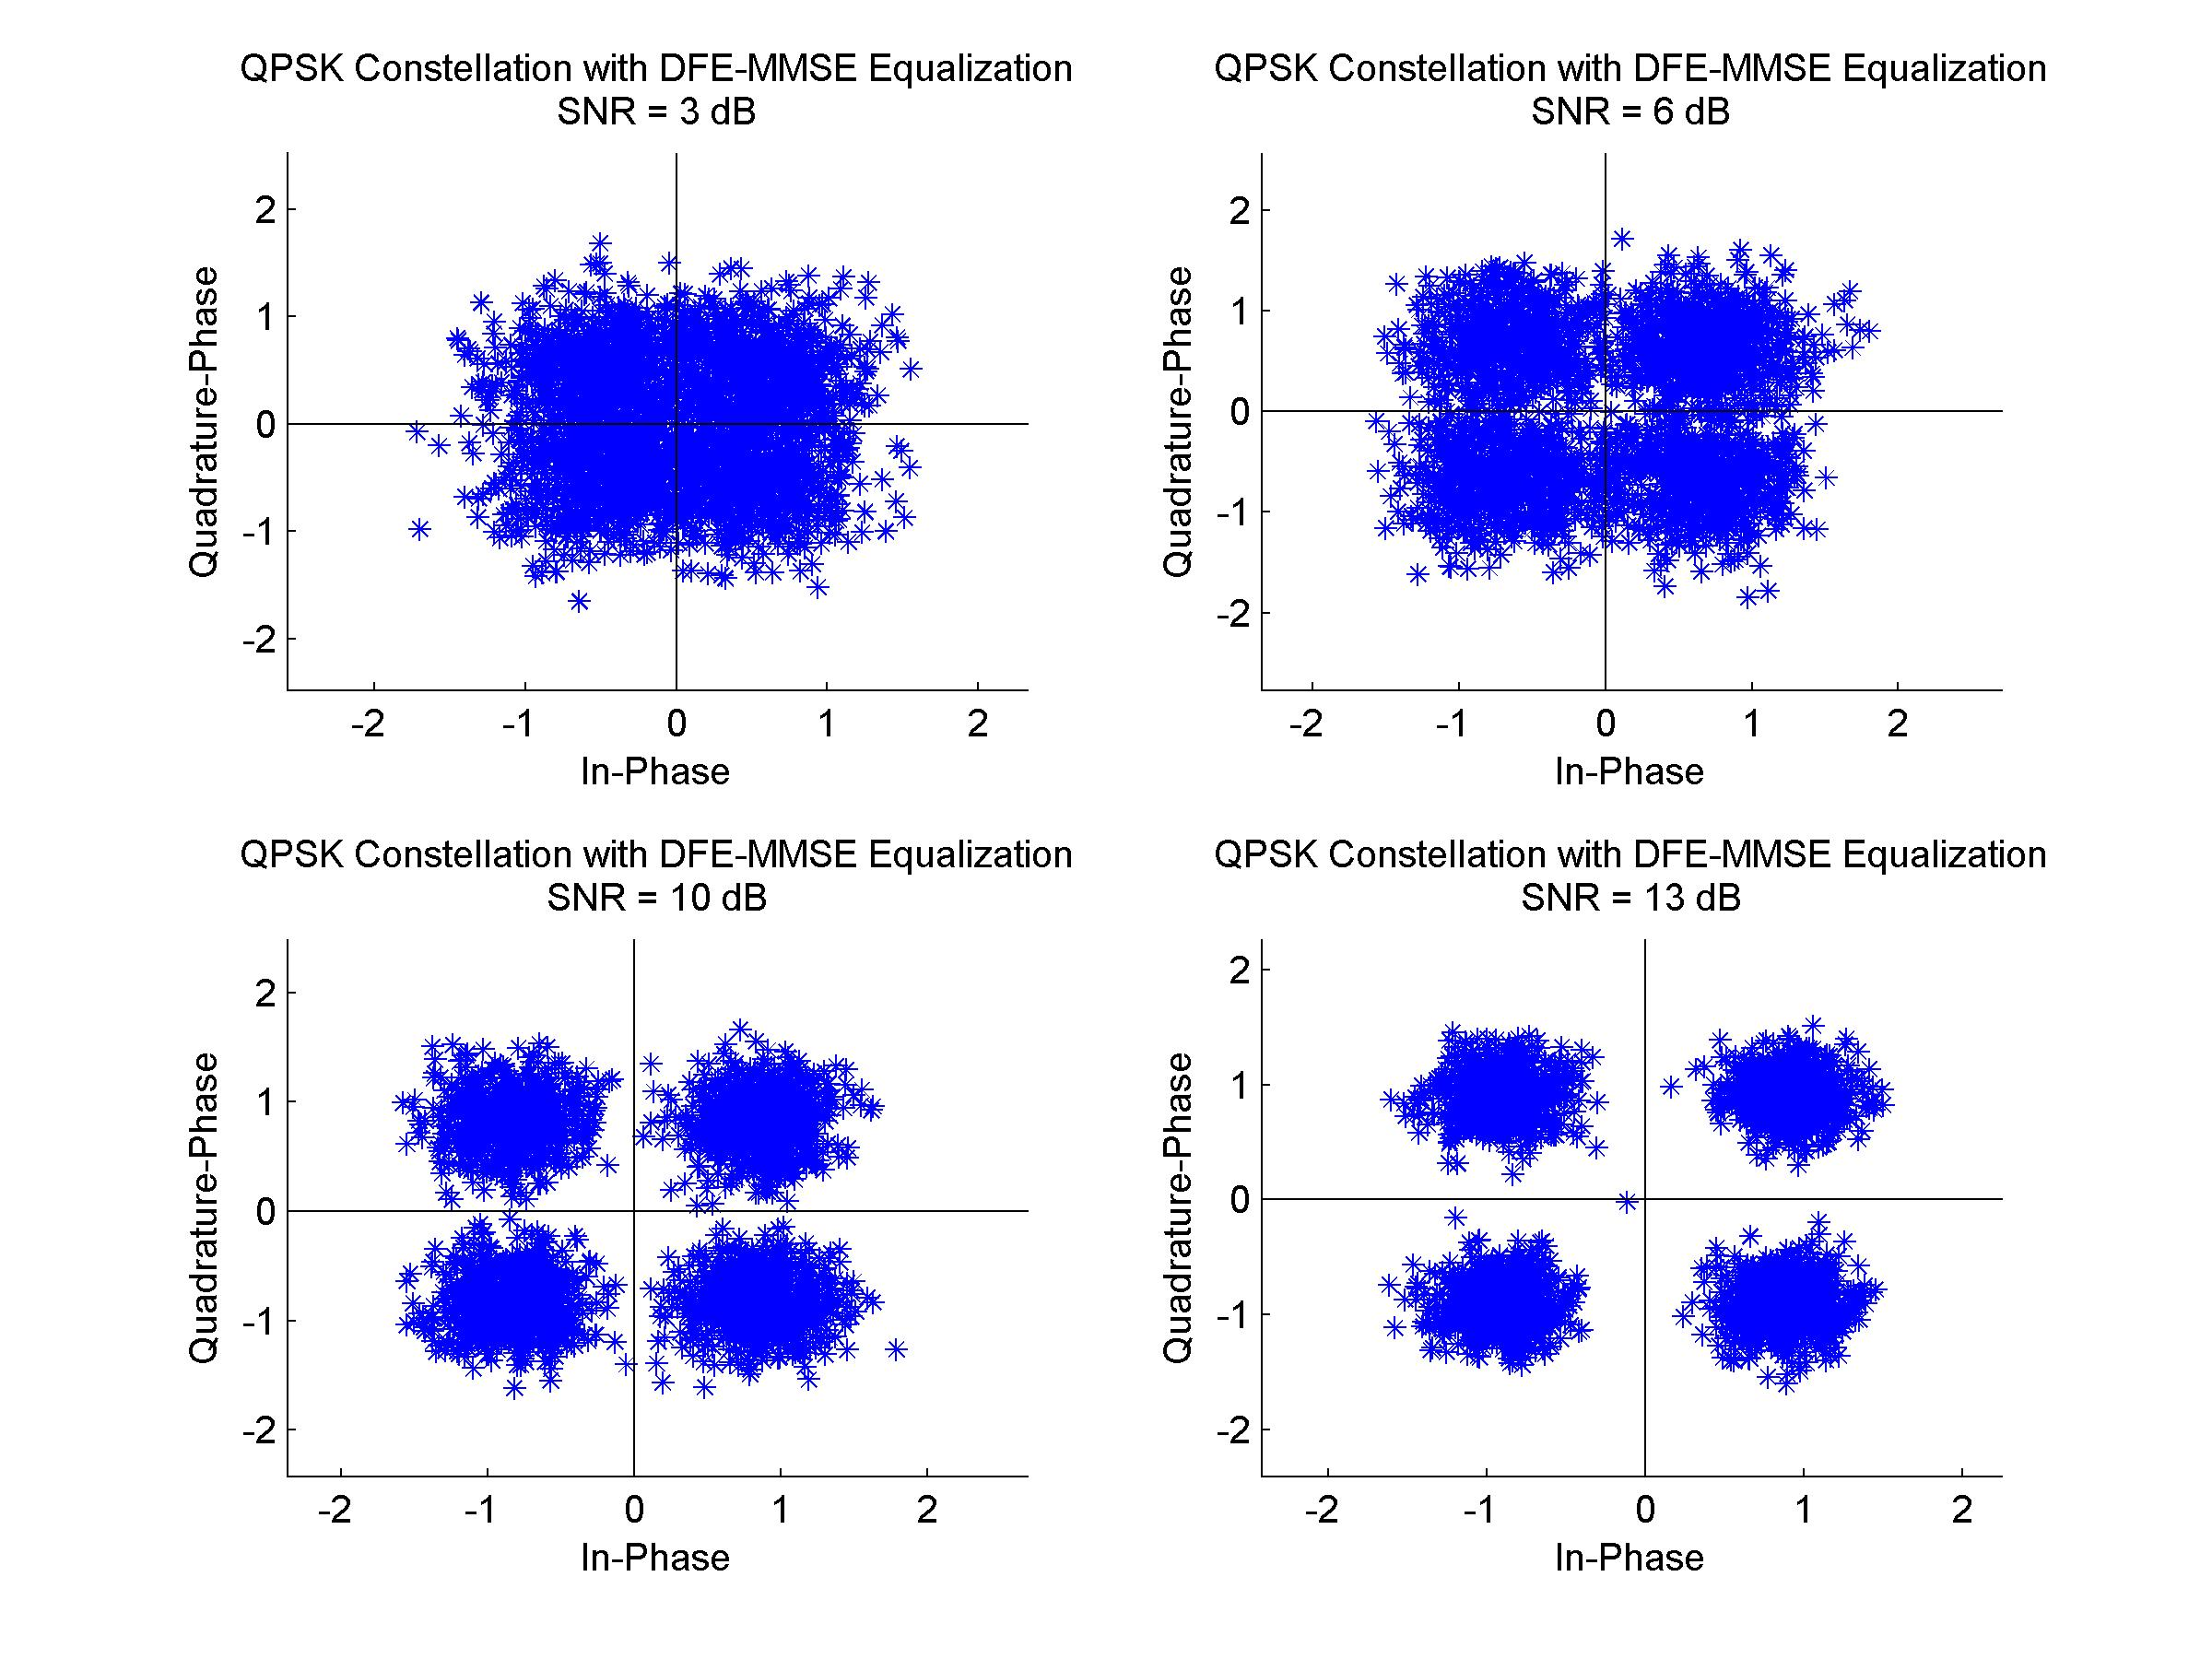
\includegraphics[width=0.7\textwidth]{qpConstDFEMMSE3.jpg}
\caption{Constellation plot for a QPSK modulated signal with MMSE-DFE equalization under channel reponse $h_3(t)$}
\end{figure}


\newpage
\section{Conclusion}
\label{sec:conc}

BLAH

\appendix
\newpage
\bibliographystyle{plain}
\bibliography{step4}
\newpage
%% the \\ insures the section title is centered below the phrase: Appendix B
%\section{Project Assignment}
%\label{app:assign}
%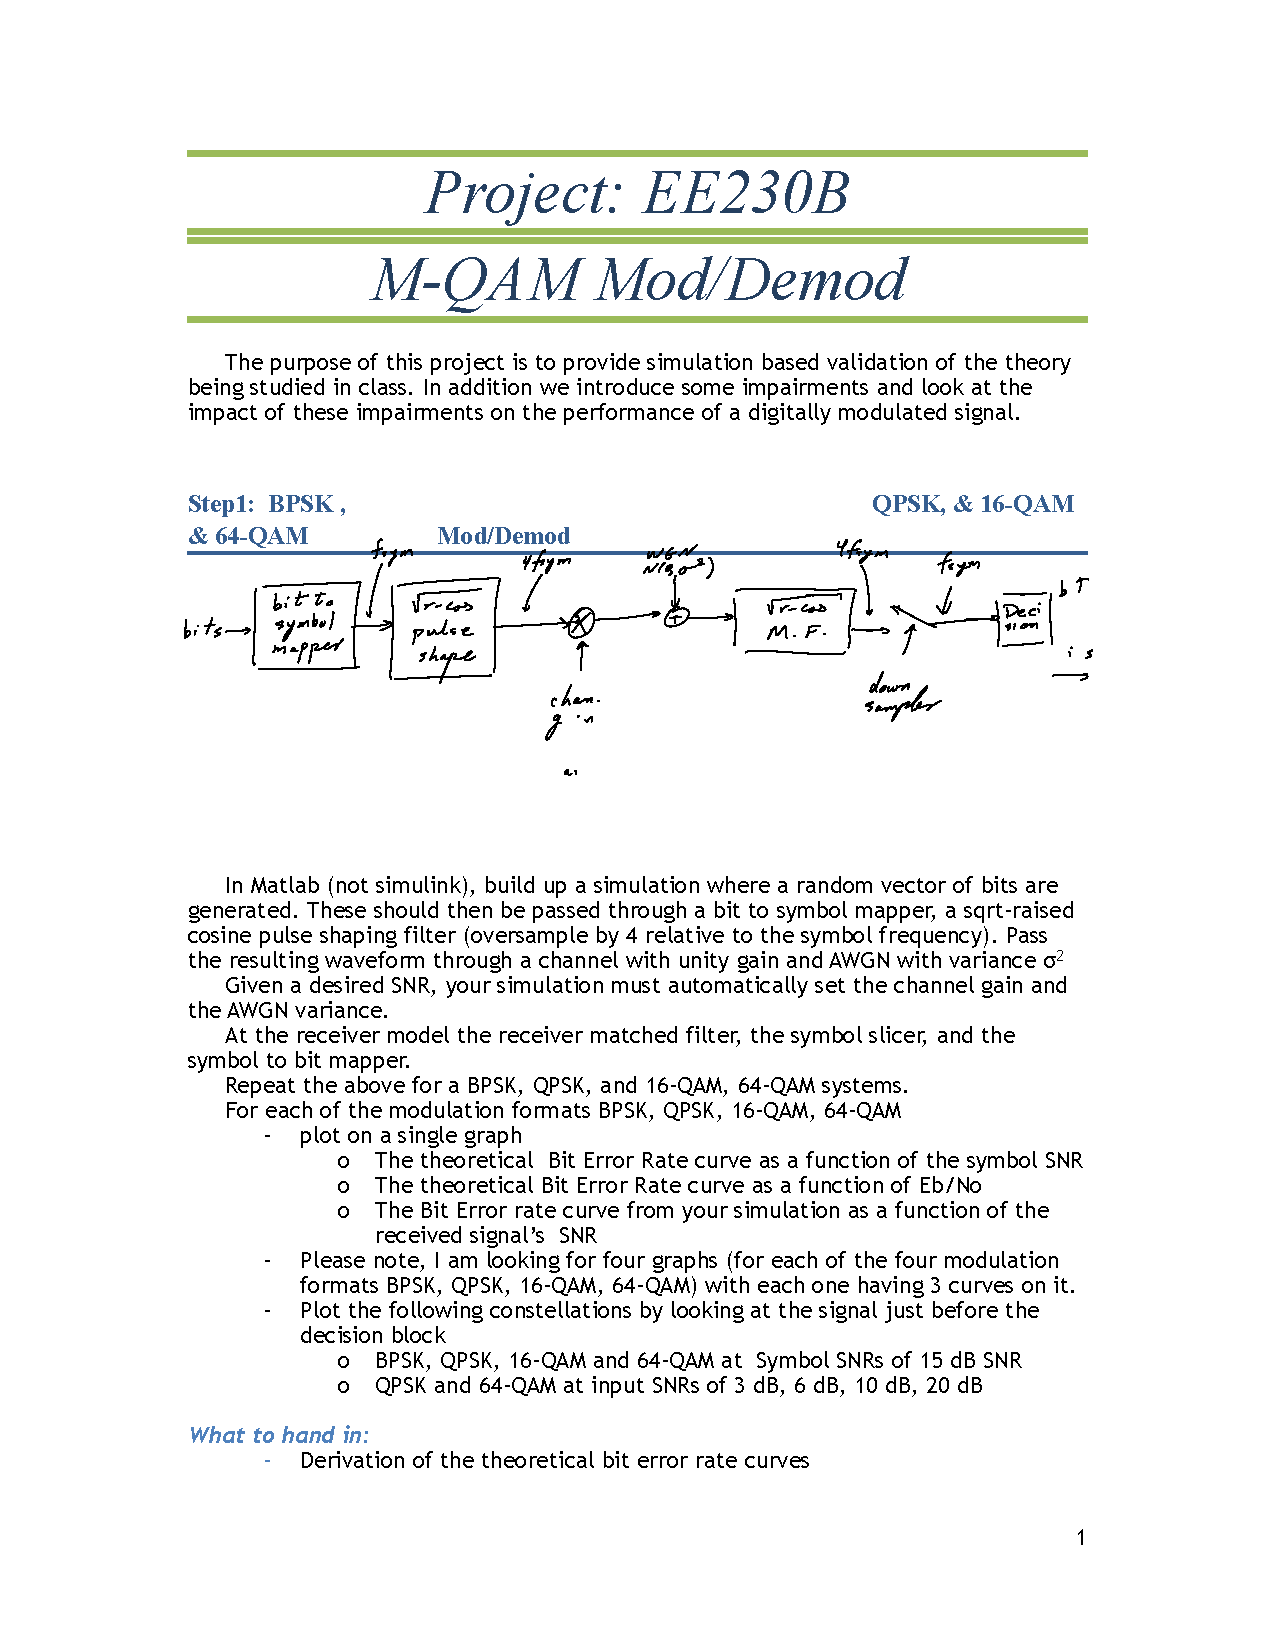
\includepdf[pages={1-5}]{project_overview.pdf}
%\cleardoublepage
%\newpage

\section{Random Bit Sequence Generator}
\label{app:random_bit_generator}
\lstinputlisting{random_bit_generator.m}

\section{Bit to Symbol Mapper}
\label{app:bittosym}
\subsection{BPSK Modulation}
\label{app:bpsk_mod}
\lstinputlisting{bpsk_mod.m}

\subsection{QPSK Modulation}
\label{app:qpsk_mod}
\lstinputlisting{qpsk_mod.m}

\section{Up Sampler}
\label{app:impulse_train}
\lstinputlisting{impulse_train.m}

\section{Square Root Raised Cosine Filter}
\label{app:sqrt_raised_cosine}
\lstinputlisting{sqrt_raised_cosine.m}

\section{Additive Gaussian White Noise Channel}
\label{app:awgn_channel}
\lstinputlisting{awgn_complex_channel.m}

\section{Sampler}
\label{app:sampler}
\lstinputlisting{sampler.m}

\section{Decision Block}
\label{app:dblocks}
\subsection{BPSK Demodulation}
\label{app:bpsk_demod}
\lstinputlisting{bpsk_demod.m}

\subsection{QPSK Demodulation}
\label{app:qpsk_demod}
\lstinputlisting{qpsk_demod.m}


\section{Equalizers}
\subsection{ZF Equalizer}
\lstinputlisting{ZFEqualizer.m}
\subsection{MMSE Equalizer}
\lstinputlisting{MMSE_Equalizer.m}
\subsection{MMSE-DFE Equalizer}
\lstinputlisting{MMSE_Equalizer_Train.m}


\section{Simulations}
\subsection{BPSK Simulation}
\lstinputlisting{step5_sim_bpsk.m}

\subsection{QPSK Simulation}
\lstinputlisting{step5_sim_qpsk.m}

\end{document}
